%instiki:category: FisicaSubatomica
% use latex2itexv2 chapter1.tex to obtain inkstiki file
% use latex2itexTOC to obtain Tabla de Contenidos
%%%%%%%%%% TODO %%%%%%%%%%%%
%% Dejar sólo los resultados matématicos.
%% Mover la discusión del campo escalar complejo al capítulo 2 y demostrar allí
%% que la corriente para una transformación global es la misma que para una local
%% con derivada covariante incluida. El campo escalar siempre puede hacer referencia
%% al par de Cooper
%% Quitar toda referencia a la Ecuación de Schrodinger y deducir todos
%% los postulados en el contexto de fermiones de Weyl
%% Ilustrar el Lagrangiano de Schrodinger como límite no relativista del
%% Lagrangiano de Dirac o algo así
\chapter{Teoría Clásica de Campos}
\label{chap:tcc} %náinstiki
%instiki:
%instiki:***
%instiki:
%instiki:[[NotasFS|Tabla de Contenidos]]
%instiki:
%instiki:***
%instiki:
%generated with html2itexTOC instiki_source.html
%instiki:* [Principio de M\'\i nima Acci\'on](#la)
%instiki:
%instiki:* [La cuerda cl\'asica unidimensional](#la-cuerda-clasica)
%instiki:
%instiki:* [Principio de M\'\i nima Acci\'on para ...](#principio-de-minima-call)
%instiki:
%instiki:* [Aplicaci\'on a Mec\'anica Cu\'antica](#aplic-mecan-cuant)
%instiki:
%instiki:* [Aplicaci\'on a la cuerda unidimenisonal](#aplicacion-la-cuerda)
%instiki:
%instiki:***
Mostraremos la conexión entre teoría clásica de campos y la relatividad
especial.  
%instiki:

% Antes de entrar en materia, se sentarán las bases teóricas necesarias sobre el sistema de unidades  más utilizado en física subatómica en la Sección~\ref{sec:NU} y temas de relatividad especial que serán utilizados posteriormente en la Sección \ref{sec:srn}. Los ejemplos te cuadrivectores en la Subsección~ se dejan como referencia para posible uso posterior

\section{Teoría de Grupos}

\subsection{Definición de grupo}
Ver \url{https://indico.cern.ch/event/243629}


\subsection{$\operatorname{SO}(2)$}



$\operatorname{SO}(2)$ es el grupo de rotaciones de dos ejes reales. Un ejemplo de transformación es la de un montaje experimental en la cual se determina el movimiento de un cuerpo con respecto a los ejes $x$, $y$ correpondientes a los lados de la mesa ilustrado en la figura~\ref{fig:tabla} izquierda. Posteriormente se repite la medida con la mesa rotada un ángulo $\theta$ pero manteniendo la posición del montaje experimental sobre la misma, como se ilustra en la figura~\ref{fig:tabla} derecha. Es claro que la trayectoria del movimiento no depende del sistema de referencia.
\begin{figure}
  \centering
  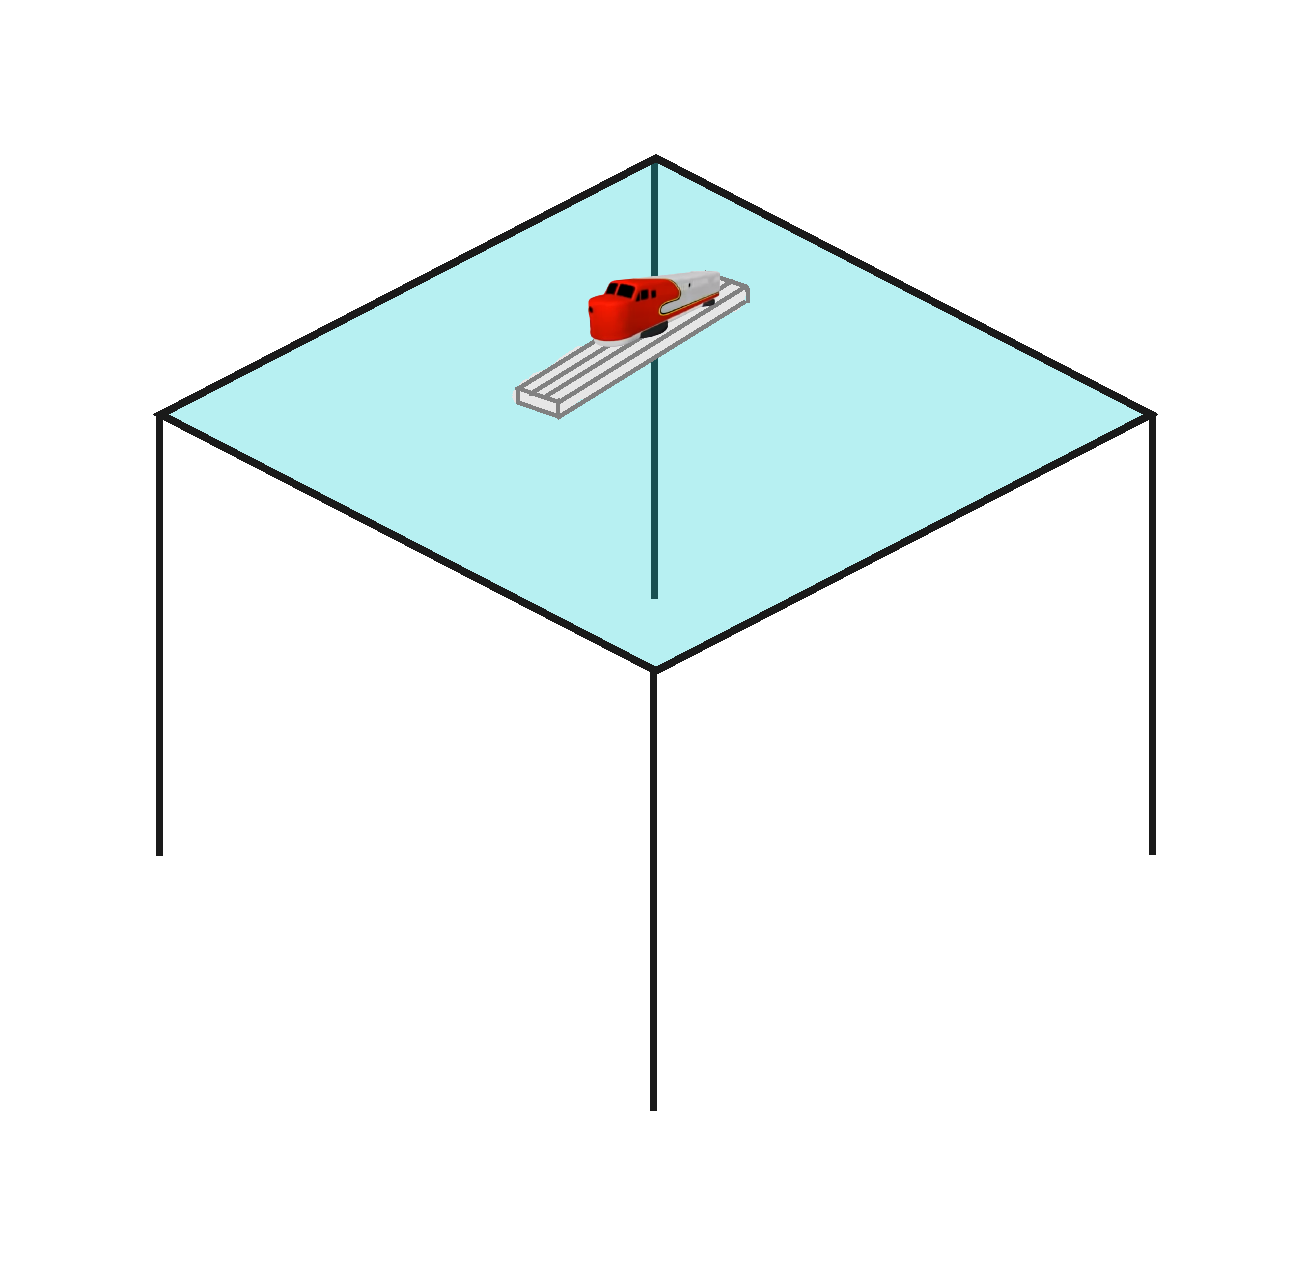
\includegraphics[scale=0.4]{table}
  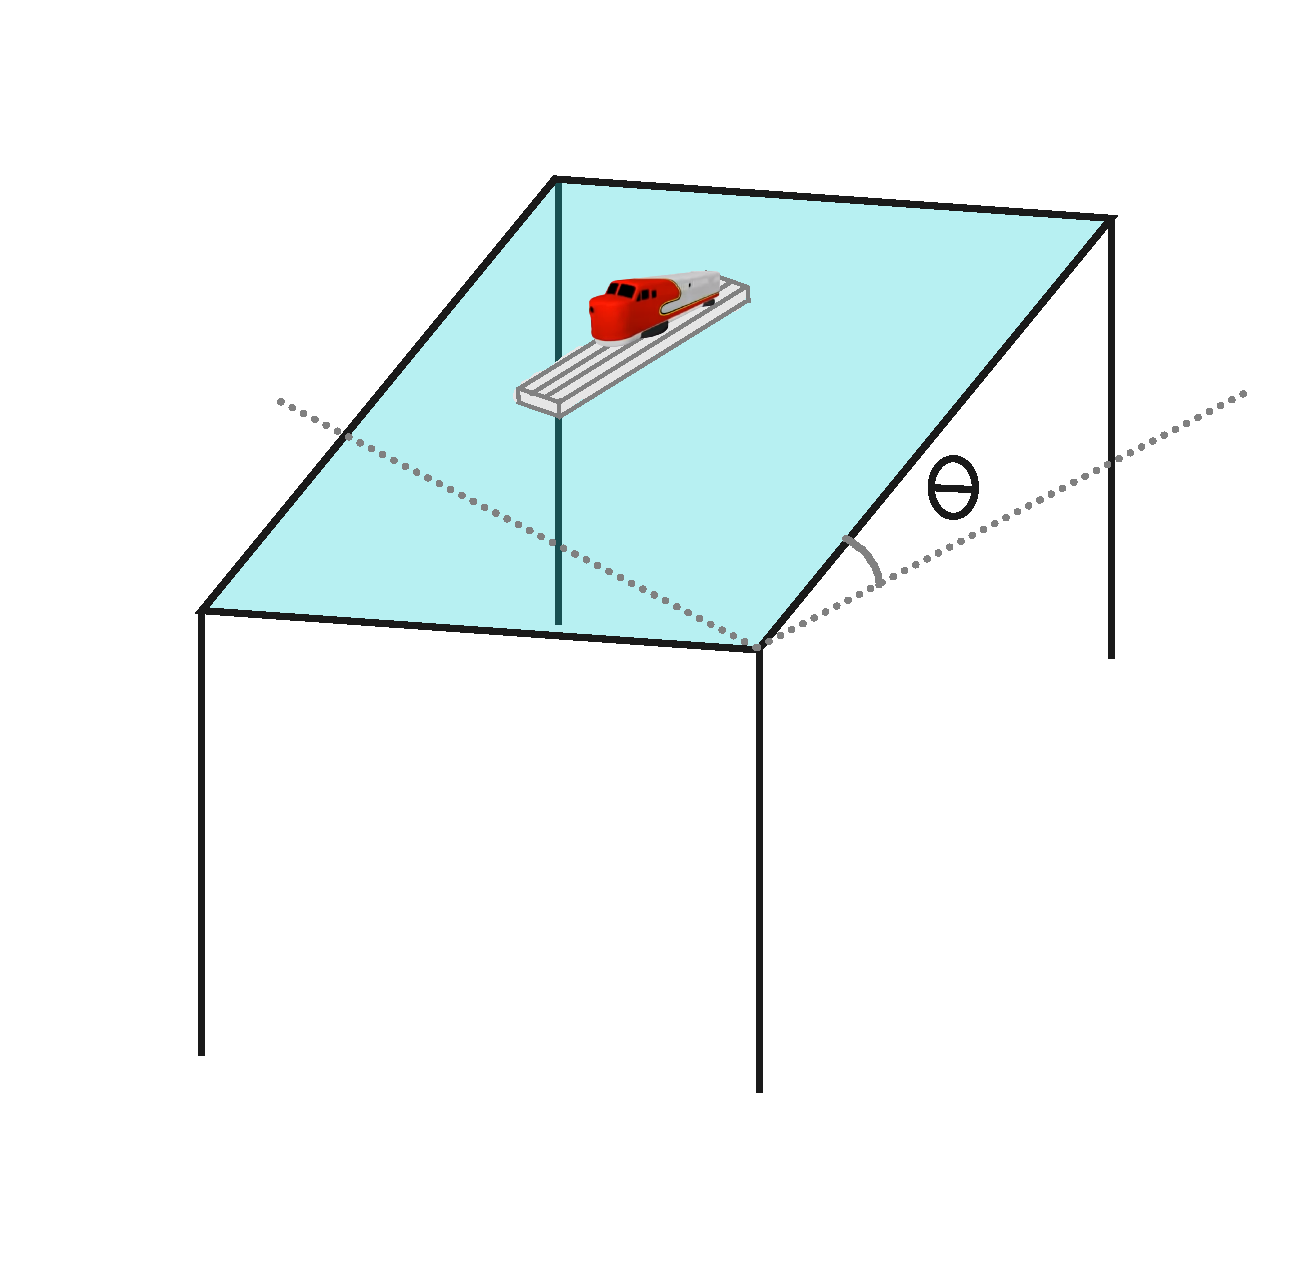
\includegraphics[scale=0.4]{tabletheta}
  \caption{Rotación de sistema de coordenadas}
  \label{fig:tabla}
\end{figure}




\begin{figure}
  \centering
  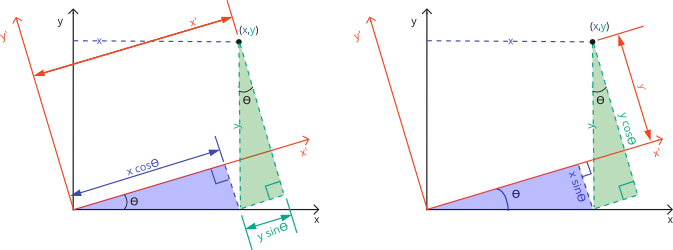
\includegraphics[scale=0.75]{so2}
  \caption{Rotación por ángulo $\theta$}
  \label{fig:so2}
\end{figure}



Considere un punto $(x,y)$ en sistema de referencia de dos dimensiones. Si cambiamos a un sistema de referencia rotado por un ángulo $\theta$, $(x',y')$, como se muestra en la figura~\ref{fig:so2}, podemos definir los dos triángulos rectángulos que se muestran en la figura y a partir de ellos obtener la transformación de los sistemas de referencia debido a la rotación
\begin{align}
  x'=&x\cos\theta+y\sin\theta \nonumber\\
  y'=&y\cos\theta-x\cos\theta\,.
\end{align}
En forma matricial, la transformación del sistema de coordenas inicial al sistema de coordenados rotado por un ángulo $\theta$ está dado por
\begin{align}
  \begin{pmatrix}
    x'\\
    y'\\
  \end{pmatrix}=
  \begin{pmatrix}
    \cos\theta & \sin\theta\\
    -\sin\theta& \cos\theta\\
  \end{pmatrix}
  \begin{pmatrix}
    x\\
    y\\
  \end{pmatrix}.
\end{align}

\begin{frame}[fragile,allowframebreaks]
Una representación matricial de $\operatorname{SO}(2)$, corresponde al Grupo de matrices $2\times 2$ ortogonales de determinante 1
\begin{align*}
  R(\theta)=
  \begin{pmatrix}
  \cos\theta &\sin\theta\\  
  -\sin\theta&\cos\theta\\  
  \end{pmatrix},
\end{align*}
donde
\begin{align*}
  R^{-1}(\theta)=& R^{\operatorname{T}}(\theta)=R(-\theta)
=
  \begin{pmatrix}
  \cos\theta &-\sin\theta\\  
  \sin\theta&\cos\theta\\  
  \end{pmatrix}, & \det[R(\theta)]=&\cos^2\theta+\sin^2\theta=1\,.
\end{align*}

Éste es  un grupo continuo. Por lo tanto se puede generar a partir de transformaciones infinitesimales.
% \end{frame}
% \begin{frame}[fragile,allowframebreaks]
Para ello,
considere el generador del Grupo de Rotaciones en dos dimensiones
\begin{align}
  \label{eq:ieab}
(\tau)_{ab}=-i \epsilon_{ab}\,, 
\end{align}
tal que
\begin{align*}
\epsilon_{ac}\epsilon_{cb}=-\delta_{ab}\,.
\end{align*}
Entonces  

\begin{align}
  \label{eq:so2g}
  \tau=
  \begin{pmatrix}
   0 & -i \\
   i & 0 \\    
  \end{pmatrix},
\end{align}
\end{frame}
con álgebra
\begin{align}
  \tau^2=&\boldsymbol{1}_{2\times2}=
  \begin{pmatrix}
    1 & 0\\
    0 & 1\\
  \end{pmatrix}. 
\end{align}
Por consiguiente
\begin{align*}
  \tau^3=&  \begin{pmatrix}
    0 & -i\\
    i & 0\\
  \end{pmatrix}=\tau\,.
\end{align*}

\begin{frame}[fragile,allowframebreaks]

  

Definimos una representación matricial del Grupo de las rotaciones como
\begin{align}
  \label{eq:tye}
  R(\theta)=&\exp \left(i \tau \theta  \right) \nonumber\\
=&\sum_{n=0}^{\infty}\frac{\left(i \theta\tau \right)^{n}}{n!}\,.
\end{align}

Con está definición $R(\theta)$ is ortogonal ya que
\begin{align}
  R^{\operatorname{T}}(\theta)=& \exp \left(i \tau^{\operatorname{T}} \theta  \right) \nonumber\\
        =& \exp \left(-i \tau \theta  \right) \nonumber\\
        =&R^{-1}(\theta)\,,
\end{align}
y además
\begin{align}
  \operatorname{det}[R(\theta)]=\operatorname{det} \left[ \exp \left(i \tau \theta  \right)  \right]
  =\exp \left[ i \operatorname{Tr}(\tau) \right]=\operatorname{e}^0=1\,.
\end{align}



Para realizar la expansión de Taylor en la ec.~\eqref{eq:tye}, podemos usar la matriz de traza nula y hermítica en ec.~\eqref{eq:so2g} y generalizar sus potencias para $n$ entero
\begin{align*}
  \tau=&
  \begin{pmatrix}
   0 &-i\\ %0 &-i\\
   i &0\\  %i &0\\ 
  \end{pmatrix},&\tau^{2n}=&  \begin{pmatrix}
   1 &0\\
   0 &1\\ 
  \end{pmatrix},&\tau^{2n+1}=&  \begin{pmatrix}
   0 &-i\\
   i &0\\ 
  \end{pmatrix}.
\end{align*}
Entonces
\begin{align}
\label{eq:so2}
  R(\theta)=\exp \left( i \theta\tau \right)=&\sum_{n=0}^{\infty}\frac{\left(i \theta\tau \right)^{n}}{n!}\nonumber\\
=&\sum_{n=0}^{\infty}(i)^{2n}\frac{\left( \theta\tau \right)^{2n}}{2n!}+\sum_{n=0}^{\infty}(i)^{2n+1}\frac{\left( \theta\tau \right)^{2n+1}}{(2n+1)!}\nonumber\\
  =&\sum_{n=0}^{\infty}(-1)^{n}\frac{\theta^{2n}}{2n!}
  \begin{pmatrix}
    1 & 0\\
    0 & 1\\
  \end{pmatrix}
+\sum_{n=0}^{\infty}i(-1)^{n}\frac{ \theta^{2n+1}}{(2n+1)!}
\begin{pmatrix}
  0 & -i \\
  i & 0
\end{pmatrix}
\nonumber\\
    =&
  \begin{pmatrix}
    \cos\theta & 0\\
    0 & \cos\theta \\
  \end{pmatrix}
+
\begin{pmatrix}
  0 & \sin\theta \\
  -\sin\theta & 0
\end{pmatrix}
\nonumber\\
    =&
  \begin{pmatrix}
    \cos\theta & \sin\theta\\
     -\sin\theta& \cos\theta \\
  \end{pmatrix}
\end{align}
Este grupo es Abeliano, ya que
\begin{align}
  R(\theta_1)R(\theta_2)=R(\theta_2)R(\theta_1)
\end{align}
\end{frame}

El producto escalar entre dos vectores con respecto a un sistema inicial $(x,y)$  y un sistema final rotado  $(x', y')$ se puede obtener a partir de la rotación del sistema inercial al sistema final
\begin{align}
\begin{bmatrix}
    x\\
    y\\
  \end{bmatrix} \to  \begin{bmatrix}
    x'\\
    y'\\
  \end{bmatrix}=R(\theta)  \begin{bmatrix}
    x\\
    y\\
  \end{bmatrix} ,
\end{align}
o equivalentemente 
\begin{align}
\begin{bmatrix}
    x^1\\
    x^2\\
  \end{bmatrix}\to  \begin{bmatrix}
    x^{\prime 1}\\
    x ^{\prime 2} \\
  \end{bmatrix}=R(\theta)  \begin{bmatrix}
    x^1\\
    x^2\\
  \end{bmatrix}.
\end{align}

En componentes, tenemos
\begin{align}
  \label{eq:rso2}
  x^i\to x^{\prime i}=\sum_j{R^i}_j x^j\,.
\end{align}

Definiendo el producto escalar como
\begin{align}
  \boldsymbol{x}\cdot \boldsymbol{y}=\sum_{ij}\delta_{ij} x^i y^j,
\end{align}
podemos demostrar que es invariante bajo rotaciones. Para demostrarlo aplicamos la rotación~\eqref{eq:rso2} sobre el producto escalar rotado:
\begin{align}
  \boldsymbol{x}\cdot \boldsymbol{y}\to  \boldsymbol{x}'\cdot \boldsymbol{y}'
                     =&\sum_{ij} \delta_{ij} x^{\prime i}  y^{\prime j} \nonumber\\
                     =&\sum_{ijkl}\delta_{ij} {R^i}_k x^{k}  {R^j}_l y^{l} \nonumber\\
                     =&\sum_{ijkl} {R^i}_k \delta_{ij} {R^j}_l  x^{k}  y^{l} \nonumber\\
  =&\sum_{ikl} {R^i}_k  {R^i}_l  x^{k}  y^{l} \nonumber\\
  \label{eq:xrtrx}
                     =&\sum_{kl}  {\left( R^{\text{T}} \right)_k}^i  {R^i}_l  x^{k}  y^{l} \\
  =&\sum_{kl} x^{k}  \left( R^{\text{T}}R \right)_{kl}      y^{l} \nonumber\\
  =&\sum_{kl}  \delta_{kl}    x^{k}  y^{l} \nonumber\\
    =& \boldsymbol{x}\cdot \boldsymbol{y}\,,
\end{align}
La métrica asociada al producto escalar en este caso corresponde al delta de Kronecker $\delta_{ij}$.

En forma compacta, usando \eqref{eq:xrtrx}, tenemos que
\begin{frame}[fragile,allowframebreaks]
  si $\boldsymbol{x}$ es un vector en $\operatorname{SO(2)}$
\begin{align}
  \boldsymbol{x}\to \boldsymbol{x}'=&R \boldsymbol{x}\,,&
  \boldsymbol{x}^{\operatorname{T}}\to \boldsymbol{x}^{\prime {\operatorname{T}}}=& \boldsymbol{x}^{\operatorname{T}} R^{\operatorname{T}}\,,
\end{align}
\begin{align}
  \label{eq:psso2}
  \boldsymbol{x}\cdot \boldsymbol{x}= \boldsymbol{x}^{\operatorname{T}} \boldsymbol{x}\to \boldsymbol{x}^{\prime\operatorname{T}} \boldsymbol{x}'
  =\boldsymbol{x}^{\operatorname{T}}R^{\boldsymbol{T}} R \boldsymbol{x}=\boldsymbol{x}^{\operatorname{T}} \boldsymbol{x}\equiv  \boldsymbol{x}\cdot \boldsymbol{x}\,.
\end{align}

\end{frame}

\begin{frame}[fragile,allowframebreaks]
  En mecánica clásica el Lagrangiano es una función de escalares y por lo tanto un vector debe aparecer en forma de producto escalar, como en el caso de la energía cinética que es proporcional a $\boldsymbol{v}\cdot \boldsymbol{v}$
\end{frame}

La formulación Lagrangiana de la teoría clásica de campos que desarrollaremos a continuación hace uso también de productos escalares. Por lo tanto es conveniente definir el producto escalar en todos los espacios posibles para su uso posterior.


Hemos ilustrado como el Álgebra puede generar el grupo como tal. De hecho, podemos comenzar estableciendo de entrada el Álgebra como se hará a continuación.


\subsection{Representación fundamental}
A partir de una misma álgebra podemos definir las representaciones fundamentales de diferentes grupos. Si dos grupos diferentes provienen de la misma álgebra, diremos que dichos grupos son isomorfos.

A modo de ejemplo, para el álgebra
\begin{align}
  T^2=\operatorname{1}\,,
\end{align}
podemos definir la representación fundamental $2\times2$ del grupo $\operatorname{SO}(2)$, a partir del generador $\tau$ de la ecuación \eqref{eq:so2g}. 

El generador trivial $T=1$ nos permite definir la representación fundamental del grupo  $\operatorname{U}(1)$. Generalizando a un generador constante $T=Y$, tenemos lo siguiente.

\subsection{$\operatorname{U}(1)$}
 El Grupo $U(1)$ corresponde a las rotaciones de un eje complejo. Tiene como elementos a los números complejos de módulo 1, los cuales en coordenadas polares se puede representar como
\begin{align}
  U(\theta)=\operatorname{e}^{i \theta Y}\,,
\end{align}
donde $Y$ es el generador de los elementos del Grupo y su representación es un número real (arbitrario)\footnote{Se suele asumir que es racional}.  En este grupo, $U^{*}(\theta)=U(-\theta)$ es el inverso y $U(0)$ es la identidad.

Estos dos grupos son isomorfos: para un elemento complejo $U(\theta)$ el correspondiente elemento en $SO(2)$ es la rotación por el ángulo de cambio de fase de $U(\theta)$.

\begin{frame}[fragile,allowframebreaks]
Sea $\psi$ un \emph{vector} en el espacio $\operatorname{U}(1)$, en el sentido que puede sufrir transformaciones de cambio de fase del tipo
\begin{align}
  \psi\to \psi'=& U(\theta)\psi= \operatorname{e}^{i \theta Y}\psi \nonumber\\
  \psi^{*}\to {\psi'}^{*}=&\psi^{*} U^{*}(\theta)=\psi^{*}\operatorname{e}^{-i \theta Y}\,.
\end{align}


Podemos definir el producto escalar como
\begin{align}
  \psi\cdot \psi\equiv\psi^{*} \psi
  \to {\psi'}^{*} \psi'=\psi^{*} U^{*}(\theta) U(\theta) \psi=\psi^{*} \psi=\psi\cdot \psi\,.
\end{align}
\end{frame}

\subsection{Construcción de Grupos a partir del álgebra}
\begin{frame}[fragile,allowframebreaks]
Considere el álgebra
\begin{align}
  K^2=-\boldsymbol{1}\,,
\end{align}
Exploraremos a continuación las representaciones matriciales fundamentales de dimensión $1\times1$ y $2\times2$

\end{frame}
\subsection{$\operatorname{SO}(1)$}
\begin{frame}[fragile,allowframebreaks]
Considere el generador $1\times1$
\begin{align}
  K=-i\,,
\end{align}
que genera el elemento del grupo $\operatorname{SO}(1)$, $R(\xi)$
\begin{align}
  \lambda(\xi)=\operatorname{e^{\xi}}\,,
\end{align}
que corresponde simplemente al grupo de las exponenciales reales. Un número real puede sufrir una transformación
\begin{align}
  x\to x'=\operatorname{e^{\xi}}x\,,
\end{align}
que corresponde a su vez a un boost por la cantidad $\operatorname{e^{\xi}}$. Podemos definir un producto escalar invariante como la división de números reales tal que
\begin{align}
  x\cdot y \to x'\cdot y'\equiv \frac{x'}{y'}= \frac{\operatorname{e}^{\xi}x}{\operatorname{e}^{\xi}y}=\frac{x}{y}=x\cdot y\,.
\end{align}
\end{frame}

\subsection{$\operatorname{SO}(1,1)$}
\begin{frame}[fragile,allowframebreaks]
Queremos obtener una representación $2\times2$ del álgebra
\begin{align}
  K^2=-\boldsymbol{1}\,,
\end{align}
donde $K$ es el único generador. Para hallar una representación de esta álgebra en términos de matrices $2\times2$ considere el generador
\begin{align}
  K=&  \begin{pmatrix}
   0 &-i\\
   -i &0\\ 
  \end{pmatrix}. 
\end{align}
que genera un elemento del grupo $\operatorname{SO}(1,1)$ con parámetro $\xi$
\begin{align}
  \Lambda=\exp \left( i \xi K \right)\,.
\end{align}
Para realizar la expansión de Taylor, considere

\begin{align*}
  K^{0}=&\boldsymbol{1}_{2\times2}\,,&K=&
  \begin{pmatrix}
   0 &-i\\ %0 &-i\\
   -i &0\\  %i &0\\ 
  \end{pmatrix},&K^{2}=&  \begin{pmatrix}
   -1 &0\\
   0 &-1\\ 
  \end{pmatrix},&K^{3}=&  \begin{pmatrix}
   0 &i\\
   i &0\\ 
  \end{pmatrix},\ldots \nonumber\\
  K^{2n}=&(-1)^{n}\boldsymbol{1}_{2\times2}\,,&&
&&&K^{2n+1}=& (-1)^{n} \begin{pmatrix}
   0 &-i\\
   -i &0\\ 
  \end{pmatrix}. 
\end{align*}

Entonces,
\begin{align}
  \label{eq:km1}
  \Lambda=\exp \left( i \xi K \right)=&\sum_{n=0}^{\infty}\frac{\left(i \xi K \right)^{n}}{n!}\nonumber\\
=&\sum_{n=0}^{\infty}(i)^{2n}\frac{\left( \xi K \right)^{2n}}{2n!}+\sum_{n=0}^{\infty}(i)^{2n+1}\frac{\left( \xi K \right)^{2n+1}}{(2n+1)!}\nonumber\\
  =&\sum_{n=0}^{\infty}(-1)^{n}\frac{\xi^{2n}}{2n!}(-1)^{n}
  \begin{pmatrix}
    1 & 0\\
    0 & 1\\
  \end{pmatrix}
+\sum_{n=0}^{\infty}i(-1)^{n}\frac{ \xi^{2n+1}}{(2n+1)!} (-1)^{n}
\begin{pmatrix}
  0 & -i \\
  -i & 0
\end{pmatrix} 
\nonumber\\
  =&\sum_{n=0}^{\infty}\frac{\xi^{2n}}{2n!}
  \begin{pmatrix}
    1 & 0\\
    0 & 1\\
  \end{pmatrix}
+\sum_{n=0}^{\infty}\frac{ \xi^{2n+1}}{(2n+1)!} 
\begin{pmatrix}
  0 & 1 \\
  1 & 0
\end{pmatrix} 
\nonumber\\
  =&
  \begin{pmatrix}
    \cosh\xi & 0\\
    0 & \cosh\xi \\
  \end{pmatrix}
+
\begin{pmatrix}
  0 & \sinh\xi \\
  \sinh\xi & 0
\end{pmatrix}
\nonumber\\
    =&
  \begin{pmatrix}
    \cosh\xi & \sinh\xi\\
     \sinh\xi& \cosh\xi \\
  \end{pmatrix},
\end{align}
Podemos entonces definir el grupo $\operatorname{SO}(1,1)$ como el grupo de las matrices $2\times2$ que satisfacen la condición
\begin{align}
  \Lambda^T g \Lambda=g\,,
\end{align}
donde
\begin{align}
  g=
  \begin{pmatrix}
    1 & 0\\
    0 & -1\\
  \end{pmatrix}.
\end{align}
\end{frame}

\begin{frame}[fragile,allowframebreaks]
  Si $\boldsymbol{x}=
  \begin{pmatrix}
    x^0& x^1
  \end{pmatrix}^{\operatorname{T}}
$ es un vector en $\operatorname{SO}(1,1)$
\begin{align}
  \boldsymbol{x}\to \boldsymbol{x}'=&\Lambda \boldsymbol{x}\,,&
  \boldsymbol{x}^{\operatorname{T}}\to \boldsymbol{x}^{\prime {\operatorname{T}}}=& \boldsymbol{x}^{\operatorname{T}} \Lambda^{\operatorname{T}}\,,
\end{align}
\begin{align}
  \label{eq:psso11}
  \boldsymbol{x}\cdot \boldsymbol{x}= \boldsymbol{x}^{\operatorname{T}}g \boldsymbol{x}\to \boldsymbol{x}^{\prime\operatorname{T}}g \boldsymbol{x}'
  =\boldsymbol{x}^{\operatorname{T}}\Lambda^{\boldsymbol{T}}g \Lambda \boldsymbol{x}=\boldsymbol{x}^{\operatorname{T}}g \boldsymbol{x}\equiv  \boldsymbol{x}\cdot \boldsymbol{x}\,.
\end{align}
\end{frame}
de manera que el producto escalar es
\begin{align}
  \boldsymbol{x}\cdot \boldsymbol{x}=&\sum_{\mu,\nu}g_{\mu\nu}x^{\mu}x^{\nu}\,,& \mu,\nu=0,1\,.
\end{align}
donde $g_{\mu\nu}$, correspondiente a las componentes de la matrix $2\times2$ $g$, es la métrica del producto
escalar bajo $\operatorname{SO}(1,1)$.

El diagrama mostrado en la figura~\ref{fig:sunson} resume los grupos introducidos hasta ahora, presenta los que discutiremos a continuación y la correspondiente generalización a dimensión $N$.
\begin{frame}[fragile,allowframebreaks]
\begin{figure}
  \centering
  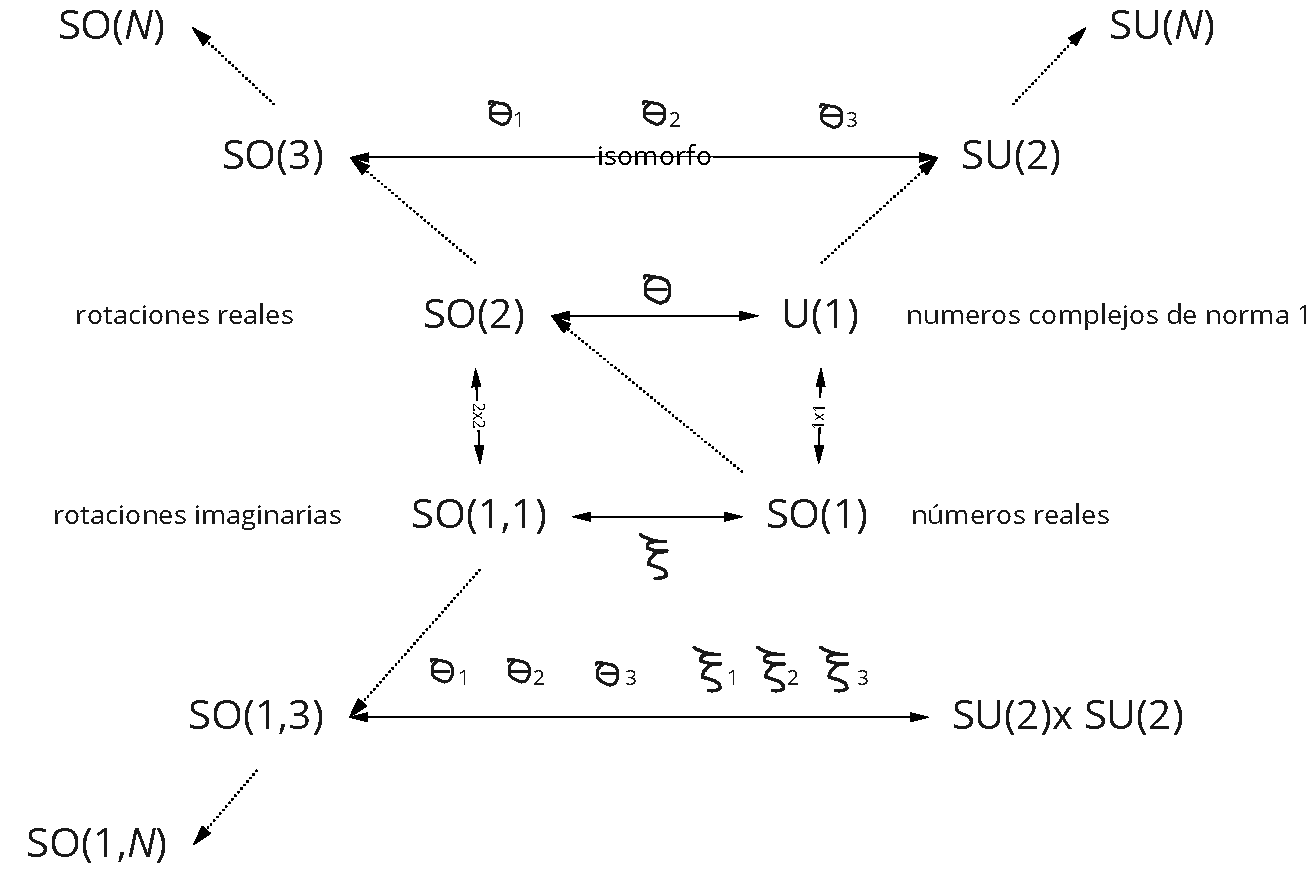
\includegraphics[scale=0.65]{sunson}
  \caption{Grupos de Lie}
  \label{fig:sunson}
\end{figure}
\end{frame}


\subsection{$\operatorname{SO}(3)$}
Una representación matricial de esta álgebra se puede obtener con la llamada representación adjunta del Grupo de rotaciones en 3 dimensiones, $\operatorname{SO}(3)$, definida a partir de las constantes de estructura \cite{Veltman}
\begin{frame}[fragile,allowframebreaks]
\begin{align}
  \label{eq:so3adj}
  (L^i)_{jk}=-i\epsilon_{ijk}\,.
\end{align}
Explícitamente
\begin{align*}
  L^1=&
  \begin{pmatrix}
   0 & 0 & 0\\
   0 & 0 & -i\\
   0 & i & 0 \\
  \end{pmatrix}&
 L^2=&
 \begin{pmatrix}
  0 & 0  & i \\ 
  0 & 0  & 0 \\
 -i & 0  & 0 \\
 \end{pmatrix}&
 L^3=&
 \begin{pmatrix}
   0 & -i & 0\\
   i & 0  & 0\\
   0 & 0 & 0\\
 \end{pmatrix}
\end{align*}

Estos generadores satisfacen el álgebra (suma sobre índices repetidos)
\begin{align}
  %the summation only includes a term
  \left[ L^i,L^j \right]=& i \epsilon_{ijk}L^{k}\,.
\end{align}
\end{frame}
Estos generan los elementos de $SO(3)$
\begin{align}
  R(\boldsymbol{\theta})=&\exp(i \theta_j L^{j}),\qquad\text{sum in $j$}\nonumber\\
                 =&\exp(i\theta_1 L_1+i\theta_2 L_2+i\theta_3 L_3)\,.
\end{align}

Para aislar los subgrupos de un parámetro definimos:
\begin{align}
  R_i\equiv R(\theta_i)
\end{align}
\begin{frame}[fragile,allowframebreaks]
donde, haciendo los mismos pasos que para $SO(2)$ en \eqref{eq:so2},
\begin{align}
  \label{eq:lirot}
  R(\theta_1)=&
  \begin{pmatrix}
   1 &   0        &0\\
   0 &\cos\theta_1  & \sin\theta_1\\
   0 & -\sin\theta_1& \cos\theta_1\\
  \end{pmatrix},\quad R(\theta_2)=
  \begin{pmatrix}
     \cos\theta_2 &0& -\sin\theta_2\\
     0          &1& 0          \\
    \sin\theta_2  &0&  \cos\theta_2\\
  \end{pmatrix}\quad R(\theta_3)=
  \begin{pmatrix}
     \cos\theta_3 & \sin\theta_3&0\\
     -\sin\theta_3& \cos\theta_3&0\\
      0         &     0     &1\\
  \end{pmatrix}\,,
\end{align}
\end{frame}
que corresponden respectivamente a rotaciones sobre el eje $x$ por un ángulo $\theta_1$, sobre el eje $y$ por un ángulo $\theta_2$, sobre el eje $z$ por un ángulo $\theta_3$.

Sin perdida de generalidad, un elemento del grupo $\operatorname{SO}(3)$, es decir, una matriz $3\times3$ ortogonal de determinante 1, $R(\boldsymbol{\theta})$, se puede definir como el producto de las anteriores matrices de rotación de un parámetro
\begin{frame}[fragile,allowframebreaks]
\begin{align}
 R(\boldsymbol{\theta}) =&R(\theta_1)R(\theta_2)R(\theta_3) \nonumber\\
=&
  \begin{pmatrix}
    c_1 c_2-c_3 s_1 s_2    & c_1 c_2 + c_3 c_1 s_2  & s_3 s_2 \\
    -c_1 s_2 - c_3 s_1 s_2 & -s_1 s_2 + c_3 c_1 c_2 & s_3 c_2 \\
    s_3 s_1               & -s_3 c_1               & c_3\\
  \end{pmatrix},
\end{align}
donde $c_i=\cos \theta_i$,  $s_i=\sin \theta_i$.


Claramente, el Grupo $\operatorname{SO}(3)$ es no Abeliano, es decir
\begin{align*}
  R(\boldsymbol{\theta}_1)R(\boldsymbol{\theta}_2)\ne R(\boldsymbol{\theta}_2)R(\boldsymbol{\theta}_1)
\end{align*}
\end{frame}

\begin{frame}[fragile,allowframebreaks]
El producto escalar bajo $\operatorname{SO}(3)$ es invariante:
\begin{align}
  \label{eq:psso3}
  \boldsymbol{x}\cdot \boldsymbol{x}= \boldsymbol{x}^{\operatorname{T}} \boldsymbol{x}\to \boldsymbol{x}^{\prime\operatorname{T}} \boldsymbol{x}'
  =\boldsymbol{x}^{\operatorname{T}}R^{\boldsymbol{T}} R \boldsymbol{x}=\boldsymbol{x}^{\operatorname{T}} \boldsymbol{x}=  \boldsymbol{x}\cdot \boldsymbol{x}\,.
\end{align}
\end{frame}

Note que la combinación lineal se puede expresar como
\begin{align}
  i\boldsymbol{\theta}\cdot\boldsymbol{L}=& i\theta_1 L_1+i\theta_2 L_2+i\theta_3 L_3 \nonumber\\
=&   \begin{pmatrix}
  0           & \theta_3 & -\theta_2 \\
  -\theta_3   &  0       & \theta_1 \\
  \theta_2    & -\theta_1 & 0
   \end{pmatrix}.
\end{align}

Un ejemplo de vector es el vector de velocidad, $\boldsymbol{v}$. Sea $\boldsymbol{k}$ un vector unitario describiendo un eje de rotación sobre el cual $\boldsymbol{v}$ rota por un ángulo $\theta$ de acuerdo a la regla de la mano derecha como se ilustra en la figura~\ref{fig:rf}.
\begin{figure}
  \centering
  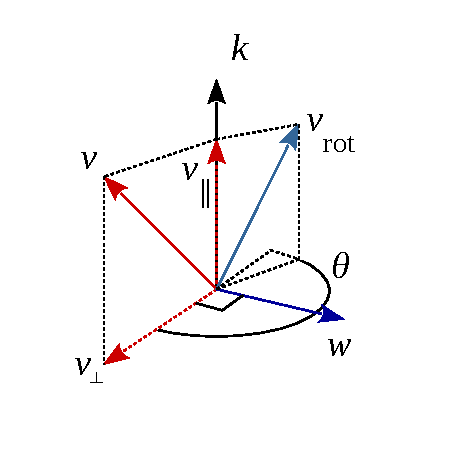
\includegraphics[scale=0.8]{Rodrigues-formula}
  \caption{Rotación vector velocidad. Tomado de \cite{rodriguez}}
  \label{fig:rf}
\end{figure}

Representado el resultado del producto vectorial $\boldsymbol{k}\times\boldsymbol{v}$ como una matrix columna,
\begin{align}
  \begin{pmatrix} (\boldsymbol{k}\times\boldsymbol{v})_x \\ (\boldsymbol{k}\times\boldsymbol{v})_y \\ (\boldsymbol{k}\times\boldsymbol{v})_z \end{pmatrix} = \begin{pmatrix} k_y v_z - k_z v_y \\ k_z v_x - k_x v_z \\ k_x v_y - k_y v_x \end{pmatrix} =& \begin{pmatrix} 0 & -k_z & k_y \\ k_z & 0 & -k_x \\ -k_y & k_x & 0 \end{pmatrix} \begin{pmatrix} v_x \\ v_y \\ v_z \end{pmatrix} \nonumber\\
=& \boldsymbol{K} \boldsymbol{v}\,,
\end{align}
donde
\begin{align}
  \boldsymbol{K}=\begin{pmatrix} 0 & -k_z & k_y \\ k_z & 0 & -k_x \\ -k_y & k_x & 0 \end{pmatrix}
\end{align}
Si definimos la matriz de rotación, $R$ perteneciente a $\operatorname{SO}(3)$, a través de un ángulo $\theta$ sobre el eje $\boldsymbol{k}$
\begin{align}
  R(\theta)=\exp \left( - i \theta i \boldsymbol{K} \right)\,,
\end{align}
entonces
\begin{align}
  R(\theta)=I+ \boldsymbol{K} \sin\theta + (1-\cos\theta)\boldsymbol{K}^2\,.
\end{align}
done $I$ es la matriz identidad. En \cite{rodriguez} se encuentra la demostración.

En general, Los objetos que sufren transformaciones en $\operatorname{SO}(N)$ son vectores en ese espacio, $\boldsymbol{x}$, que dejan el producto escalar bajo la métrica $\delta_{ij}$ del tipo~\eqref{eq:psso3} invariante.

\subsection{$\operatorname{SU}(2)$} 

La representación matricial isomorfa a $\operatorname{SO}(3)$ pero con matrices $2\times2$ corresponde al Grupo $SU(2)$ de rotaciones de dos ejes complejos.
\begin{english}
  The Pauli matrices are set of matrices satisfying this commutation relations:
\end{english}
\begin{spanish}
Las matrices de Pauli son un conjunto de matrices que satisfacen la misma álgebra de $\operatorname{SU}(2)$
\end{spanish}
\begin{frame}[fragile,allowframebreaks]
\begin{equation}
  \label{eq:paulialg}
  %summation only includes a term!
  \left[\frac{\tau^i}{2},\frac{\tau^j}{2} \right]=i\,\epsilon_{ijk}\frac{\tau^k}{2}
\end{equation}
donde $\tau^i$ 
\begin{equation}
  \label{eq:paulimatr}
  \tau_1=
  \begin{pmatrix}
    0&1\\
    1&0
  \end{pmatrix}, \qquad
 \tau_2=
  \begin{pmatrix}
    0&-i\\
    i&0
  \end{pmatrix},\qquad 
 \tau_3=
  \begin{pmatrix}
    1&0\\
    0&-1
  \end{pmatrix},
 \end{equation}

dividas por dos, corresponden a los generadores del Grupo. Las constantes de estructura del Grupo corresponden a $\epsilon_{ijk}$. Como los generadores no conmutan, $SU(2)$ es un Grupo de Lie no Abeliano. Definiendo los generadores de $SU(2)$ como
\begin{equation}
  T^i=\frac{\tau_i}{2},
\end{equation}
\end{frame}

Las matrices de Pauli y por consiguiente $T_i$ satisfacen 
\begin{align}
  \tau_i^\dagger&=\tau_i\nonumber\\
  \operatorname{Tr}  \left(
    \tau_i
  \right)&=0
\end{align}
Además
\begin{align}
  \label{eq:64qftw}
  \det
  \left(
    \tau_i
  \right)&=-1\nonumber\\
  \left\{ 
    \tau_i,\tau_j
  \right\}&=2\delta_{ij}\cdot I\Rightarrow\tau_i^2=I\nonumber \\
\operatorname{Tr} \left(\tau^i\tau^j\right)&=2\delta^{ij}\nonumber\\
\tau_i\tau_j&=i\epsilon_{ijk}\tau_k+\delta_{ij}\,.
\end{align}

\begin{frame}[fragile,allowframebreaks]
Un elemento del Grupo puede escribirse como
\begin{equation}
  \label{eq:63qft}
  U(\boldsymbol{\theta})=e^{iT^i \theta_i }\approx1+iT^i\theta_i=1+i\frac{\tau^i}{2}\theta_i\,.
\end{equation}
Como antes, $\theta_i$ son los parámetros de la transformación.  Usando las propiedades $T_i$, podemos mostrar que la representación matricial $2\times 2$, $U(\boldsymbol{\theta})$, satisface
\begin{enumerate}
\item Unitariedad: $U^{-1}(\boldsymbol{\theta})=U^{\dagger}(\boldsymbol{\theta})$. En efecto
  \begin{align*}
    U^{\dagger}(\boldsymbol{\theta})U(\boldsymbol{\theta})=&e^{-i{T^i}^{\dagger} \theta_i }e^{iT^i \theta_i }\nonumber\\
=&e^{-i T^i \theta_i }e^{iT^i \theta_i } \nonumber\\
=&e^{\mathbf{0}}\nonumber\\
=&\mathbf{1}\,,
  \end{align*}
la identidad $2\times 2$.
\item Especial (Special): Usando la formula de Jacobi para la exponencial de una matriz, $A$, $\operatorname{det}\operatorname{e}^{A}=\operatorname{e}^{\operatorname{Tr}A}$, tenemos que
  \begin{align*}
   \det[U(\boldsymbol{\theta})]=&\det\left\{\exp\left[  i \operatorname{Tr}\left( T^i \right)\theta_i \right]  \right\}\nonumber\\
                           =&e^{0}\nonumber\\
                           =&1\,.
  \end{align*}
\end{enumerate}
De esta manera $T_i$ genera el grupo de matrices $2\times 2$ unitarias y de determinante 1: $SU(2)$. 
\end{frame}

El grupo $SU(2)$ de rotaciones de dos ejes complejos, es isomorfo al Grupo $SO(3)$ de rotaciones sobre tres ejes reales.

Estas relaciones se pueden generalizar a rotaciones en mayores dimensiones.

En la fig.~\ref{fig:ee} se ilustra el momento angular total para la tierra y un electrón no relativista. El momento angular total de la tierra es la suma vectorial del momento angular orbital (alrededor del sol) y el momento angular intrínseco (la rotación de la tierra sobre eje). Ambos vectores transforman bajo rotaciones de $\operatorname{SO}(3)$.

El momento angular total del electrón (no relativista) en el átomo de Higdrógeno es a su vez la suma vectorial del momento angular orbital (alrededor del protón) y el momento angular intrínseco del electrón.  Éste último sin embargo, transforma bajo rotaciones de $\operatorname{SU}(3)$, de manera que el campo asociado con el electrón debe ser un campo complejo: con magnitud y fase.

\begin{frame}[fragile,allowframebreaks]
\begin{figure}
  \centering
  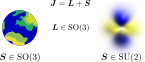
\includegraphics[scale=0.6]{JLS}
  \caption[tierra electrón]{momento angular total para la tierra y un electrón no relativista. \tiny{Créditos \url{https://www.flaticon.com/authors/smashicons} y Wikipedia}}
  \label{fig:ee}
\end{figure}
\end{frame}


\begin{frame}[fragile,allowframebreaks]
Los objetos más simples que pueden sufrir transformaciones  $\operatorname{SU}(2)$, corresponden a vectores columnas de dos objetos complejos, como dos funciones de ondas, donde cada función de onda puede tener una de dos posibilidades de carga (una carga más que en $\operatorname{U}(1)$)
\begin{align}
  \Psi=&
  \begin{pmatrix}
    \Psi_1\\
    \Psi_2
  \end{pmatrix},&
  \Psi^{\dagger}=&
  \begin{pmatrix}
    \Psi_1^{*} &
    \Psi_2^{*}
  \end{pmatrix}.                  
\end{align}

La transformación de este \emph{doblete} bajo $\operatorname{SU}(2)$ es
\begin{align}
  \Psi\to \Psi'=& U(\boldsymbol{\theta}) \Psi \nonumber\\
  \Psi^{\dagger}\to \Psi^{\prime\dagger} =& \Psi^{\dagger}U^{\dagger}(\boldsymbol{\theta}).
\end{align}
\end{frame}

La definición del producto escalar es
\begin{align}
   \Psi\cdot \Psi \equiv \Psi^{\dagger}\Psi\,. 
\end{align}

\textbf{Ejercicio:} Mostrar la invarianza del producto escalar.

\subsection{Producto escalar en $SU(2)$}
El producto escalar de $\operatorname{SU}(2)$ también se puede definir en términos de una métrica.

\begin{frame}[fragile,allowframebreaks]
  Sean $\Psi$ y $\Upsilon$, dobletes $\operatorname{SU}(2)$. Hemos definido el producto escalar $SU(2)$ de la forma $\Psi^{\dagger}\Upsilon$, por ejemplo. Pero hay otra forma de construir el producto escalar para $\operatorname{SU}(2)$. Más específicamente, tenemos
\begin{align}
  \Psi=&
  \begin{pmatrix}
    \Psi_1\\
    \Psi_2\\
  \end{pmatrix},&
  \Upsilon=&
  \begin{pmatrix}
    \Upsilon_1\\
    \Upsilon_2\\
  \end{pmatrix}.
\end{align}
Podemos definir un producto que es invariante bajo $\operatorname{SU}(2)$ como el producto escalar bajo la ``métrica'' de $\operatorname{SU}(2)$ (suma sobre índices repetidos)
\begin{align}
\Psi\cdot\Upsilon=\epsilon^{ab}\Psi_a \Upsilon_b\to \epsilon_{ab}\Psi'_a \Upsilon'_b=&\epsilon_{ab}U_{ac}U_{bd}\Psi_c \Upsilon_d\nonumber\\
  =&\left( U_{11}U_{22}-U_{12}U_{21} \right)\left(\Psi_1\Upsilon_2-\Psi_2\Upsilon_1  \right)\nonumber\\
  =&\epsilon^{ab}\left( \det\mathbf{U} \right) \Psi_a \Upsilon_b\nonumber\\
  =&\epsilon^{ab} \Psi_a \Upsilon_b\,.
\end{align}
Es claro además que
\begin{align}
 \Psi\cdot\Upsilon= \epsilon^{ab}\Psi_a \Upsilon_b=&\Psi_1 \Upsilon_2-\Psi_2 \Upsilon_1 \,.
 \end{align}


 Con el contenido de campos de $\Psi$, siempre es posible definir el doblete adjunto de $\operatorname{SU}(2)$ como 
\begin{align}
\label{eq:conjA}
 \widetilde{\Psi}\equiv & \begin{pmatrix}
                  \Psi_2^{*}\\
                 -\Psi_1^{*}\\
                \end{pmatrix}
\end{align}
En tal caso es posible escribir el producto escalar $\operatorname{SU}(2)$ es una forma matricial, la cual muestra una invarianza más evidente
\begin{align}
\widetilde{\Psi}\cdot \Upsilon\equiv \epsilon^{ab}\widetilde{\Psi}_a \Upsilon_b=&\widetilde{\Psi}_1 \Upsilon_2-\widetilde{\Psi}_2 \Upsilon_1 \nonumber\\
                     =&\Psi_2^{*}\Upsilon_2 -(-\Psi_1^{*}) \Upsilon_1 \nonumber\\
                     =&\Psi_2^{*}\Upsilon_2 +\Psi_1^{*} \Upsilon_1 \nonumber\\
                     =&\Psi_2^{*}\Upsilon_2 +\Psi_1^{*} \Upsilon_1 \nonumber\\
                     =&\delta^{ac}\Psi_a^{*}\Upsilon_c \nonumber\\
                     =&\Psi^{\dagger} \Upsilon\,.
 \end{align}

Por lo tanto, el producto escalar entre dos dobletes de $\operatorname{SU}(2)$ se puede escribir en cualquiera de las dos formas
\begin{align}
  \widetilde{\Psi}\cdot \Upsilon\,, \qquad\text{or}   \qquad \Psi^{\dagger}\Upsilon\,.
\end{align}
En adelante, usaremos la primera forma.

\textbf{Ejemplo}: Escribir $\Psi\cdot \Upsilon$ en forma matricial
\begin{align}
  \label{eq:2to2}
\Psi\cdot \Upsilon\equiv \epsilon^{ab}{\Psi}_a \Upsilon_b=&{\Psi}_1 \Upsilon_2-{\Psi}_2 \Upsilon_1 \nonumber\\
                     =&-\left(\Psi_2 \Upsilon_1 - (-\Psi_1) \Upsilon_2\right) \nonumber\\
                     =&-\begin{pmatrix}
                        \Psi_2 & -\Psi_1\\ 
                        \end{pmatrix}^{\operatorname{T}}
                         \begin{pmatrix}
                           \Upsilon_1\\
                           \Upsilon_2\\
                         \end{pmatrix} \nonumber\\
                     =&-\begin{pmatrix}
                        \Psi_2^* & -\Psi_1^*\\ 
                        \end{pmatrix}^{\dagger}
                         \begin{pmatrix}
                           \Upsilon_1\\
                           \Upsilon_2\\
                         \end{pmatrix} \nonumber\\
                     =&-\widetilde{\Psi}^\dagger \Upsilon\,.
\end{align}

Usando la correspondiente identidad para los delta de Kronecker
\begin{align}
   \epsilon^{ab}\widetilde{\Psi}_{a} \Upsilon_{b} =&\delta^{ac}\Psi_a^{*}\Upsilon_c \nonumber\\
                                     =&\epsilon^{ad}\epsilon^{cd}\Psi_a^{*}\Upsilon_c \,,
 \end{align}
y con el intercambio $a\leftrightarrow d$, tenemos que
\begin{align}
  \widetilde{\Psi}_{a} \left( \epsilon^{ab}\Upsilon_{b}\right)=&\epsilon^{da}\epsilon^{ca}\Psi_d^{*}\Upsilon_c \nonumber\\
=&\epsilon^{ad}\epsilon^{ac}\Psi_d^{*}\Upsilon_c \nonumber\\
=&\epsilon^{ad}\Psi_d^{*}\left( \epsilon^{ac}\Upsilon_c \right)\,.
\end{align}
Por consiguiente
\begin{align}
\widetilde{\Psi}_a=& \epsilon^{ad}\Psi_d^{*} \,.
\end{align}
En forma matricial, tenemos
\begin{align}
     \widetilde{\Psi}=&\begin{pmatrix} 
                  \epsilon_{11} & \epsilon_{12}\\
                 \epsilon_{21} & \epsilon_{22}
               \end{pmatrix}
               \begin{pmatrix}
                 \Psi_1^{*}\\
                 \Psi_2^{*}\\
               \end{pmatrix}\nonumber\\
               =&i\begin{pmatrix}
                 0 & -i\\
                 i & 0
               \end{pmatrix}
               \begin{pmatrix}
                 \Psi_1^{*}\\
                 \Psi_2^{*}\\
               \end{pmatrix}\nonumber\\
             =&i \tau_2 \Psi^{*}\,.
\end{align}

\textbf{Ejemplo}: Demostrar \eqref{eq:2to2}
\begin{align}
  \widetilde{\Psi}\cdot \Upsilon^*=& \Psi^{\dagger} \Upsilon^* \nonumber\\
  i \tau_2 \Psi^*\cdot \Upsilon^* =&\Psi^{\operatorname{T}*} Y^* \nonumber\\
  -i \tau_2^* \Psi \cdot \Upsilon= & \Psi^{\operatorname{T}} Y \nonumber\\
  i \tau_2 \Psi \cdot \Upsilon=&  \Psi^{\operatorname{T}} Y \nonumber\\
  i \tau_2( i \tau_2) \Psi \cdot \Upsilon=& i \tau_2 \Psi^{*\dagger} Y \nonumber\\
   \Psi \cdot \Upsilon=& - \widetilde{\Psi}^{\dagger} Y \,.
\end{align}


\end{frame}


\subsection{$SU(N)$}

\begin{frame}[fragile,allowframebreaks]
En general, si $N^{2}-1$ generadores $\Lambda_a$, satisfacen el álgebra
\begin{align}
  \left[ \Lambda_a,\Lambda_b \right]=f_{abc}\Lambda_{c}\,,
\end{align}
con
\begin{align}
  \Lambda^{\dagger}=&\Lambda\,, & \operatorname{Tr}(\Lambda)=0\,,
\end{align}
entonces las matrices $N\times N$  
\begin{align}
  U(\boldsymbol{\theta})=\exp\left( i \Lambda_{a}\theta_{a} \right)
\end{align}
son unitarias y de determinante 1, y constituyen la representación fundamental de $SU(N)$.
\end{frame}

En el caso de $U(1)$, el único generador conmutativo satisface trivialmente el álgebra y da lugar al elemento de grupo
\begin{align}
  U(\theta)=e^{i\Lambda \theta}
\end{align}
que automáticamente tienen norma 1
\begin{align*}
|U(\theta)|^2= U^{*}(\theta)U(\theta)=1\,.
\end{align*}

\begin{frame}[fragile,allowframebreaks]
Los objetos más simples que pueden sufrir transformaciones  $\operatorname{SU}(N)$, corresponden a vectores columnas de $N$ objetos complejos, como $N$ funciones de ondas por ejemplo, donde cada función de onda puede tener una de $N$ posibilidades de carga ($N-1$ cargas más que en $\operatorname{U}(1)$)
\begin{align}
  \Psi=&
  \begin{pmatrix}
    \Psi_1\\
    \Psi_2\\
    \vdots\\
    \Psi_N\\
  \end{pmatrix},&
  \Psi^{\dagger}=&
  \begin{pmatrix}
    \Psi_1^{*} &
    \Psi_2^{*}& \cdots \Psi_N^{*} 
  \end{pmatrix}.                  
\end{align}

La transformación de este \emph{multiplete} bajo $\operatorname{SU}(N)$ es
\begin{align}
  \Psi\to \Psi'=& U(\boldsymbol{\theta}) \Psi \nonumber\\
  \Psi^{\dagger}\to \Psi^{\prime\dagger} =& \Psi^{\dagger}U^{\dagger}(\boldsymbol{\theta}),
\end{align}
donde
\begin{align}
  \boldsymbol{\theta}=\left(\theta_1,\theta_2,\cdots,\theta_{N^2-1}  \right).
\end{align}

La definición del producto escalar es
\begin{align}
   \Psi \cdot \Psi \equiv \Psi^{\dagger}\Psi\,. 
\end{align}
\end{frame}

\textbf{Ejercicio:} Mostrar la invarianza del producto escalar.


\begin{frame}[fragile,allowframebreaks]
La representación adjunta para $\operatorname{SU}(N)$ esta definida por
\begin{align}
  \left[ \widetilde{\Lambda}_a \right]_{bc}=-i f_{abc}\,.
\end{align}
\end{frame}

Definiendo $\Sigma_i$ como las matrices $3\times3$ generadores de $\operatorname{SU}(2)$ en la representación adjunta
\begin{align}
  (\Sigma_i)_{jk}=-i\epsilon_{ijk}\,,
\end{align}
hemos comprobado en la ec.~\eqref{eq:adjrepsu2} que
\begin{align}
  \left[{\Sigma_i},{\Sigma_j}\right]&=i\epsilon_{ijk}{\Sigma_k}\nonumber\\
  \left[{\Sigma_i},{\Sigma_j}\right]_{lm}&=i\epsilon_{ijk}(\Sigma_k)_{lm}\,.
\end{align}

Debemos comprobar que
\begin{align}
  \left[{\Sigma_i},{\Sigma_j}\right]&=i\epsilon_{ijk}{\Sigma_k}\nonumber\\
  \left[{\Sigma_i},{\Sigma_j}\right]_{lm}&=i\epsilon_{ijk}(\Sigma_k)_{lm}\,.
\end{align}

Ya que
\begin{align}
  \label{eq:167}
  (\Sigma_i\Sigma_j)_{lm}&=(\Sigma_i)_{lk}(\Sigma_j)_{km}=-\epsilon_{ilk}\epsilon_{jkm}=\epsilon_{ilk}\epsilon_{jmk}=\delta_{ij}\delta_{lm}-\delta_{im}\delta_{lj}\nonumber\\
  -(\Sigma_j\Sigma_i)_{lm}&=-(\Sigma_j)_{lk}(\Sigma_i)_{km}=\epsilon_{jlk}\epsilon_{ikm}=-\epsilon_{jlk}\epsilon_{imk}=-\delta_{ji}\delta_{lm}+\delta_{jm}\delta_{li}\,,
\end{align}
entonces
\begin{align}
\label{eq:adjrepsu2}
[\Sigma_i,\Sigma_j]_{lm}=& (\Sigma_i\Sigma_j-\Sigma_j\Sigma_i)_{lm}\nonumber\\
=&\delta_{il}\delta_{jm}-\delta_{im}\delta_{jl}\nonumber\\
=&\epsilon_{ijk}\epsilon_{lmk}\nonumber\\
=&i\epsilon_{ijk}(-i\epsilon_{klm})\nonumber\\
=&i\epsilon_{ijk}(\Sigma_k)_{lm}\,.
\end{align}




\section{Grupo de Lorentz: $\operatorname{SO}(1,3)$}
\label{sec:glso13}

See \url{https://indico.cern.ch/event/243629/attachments/415251/576988/L2.pdf}

\begin{frame}[fragile,allowframebreaks]
  Los seis generadores independientes del Grupo de Lorentz $\operatorname{SO}(1,3)$ se pueden definir a partir del tensor antisimétrico
\begin{align}
   \left(J^{\mu\nu}\right)_{\alpha\beta}=&i\epsilon^{\mu\nu\rho\sigma}\epsilon_{\rho\sigma\alpha\beta}\,,
\end{align}
donde se usa la convención de suma sobre índices repetidos que estén contraídos (uno como superíndice y el otro como subíndice): $\mu,\nu,\alpha,\beta=0,1,2,3$, aún en el caso de que sean índices latinos: $i,j,k=1,2,3$. 


Los seis generadores independientes satisfacen el álgebra del grupo $\operatorname{SO(1,3)}$
\begin{align}
\label{eq:lrtalg}
  \left[{J}^{\mu\nu},{J}^{\rho\sigma}\right]=&
i(g^{\nu\rho}{J}^{\mu\sigma}-g^{\mu\rho}{J}^{\nu\sigma}-g^{\nu\sigma}{J}^{\mu\rho}+g^{\mu\sigma}{J}^{\nu\rho})\,,
\end{align}
donde 
\begin{equation}
  \left\{ g^{\mu\nu} \right\}=
  \begin{pmatrix}
    1&0&0&0\\
    0&-1&0&0\\
    0&0&-1&0\\
    0&0&0&-1
  \end{pmatrix},
\end{equation}
denota la forma matricial del tensor $g^{\mu\nu}$.  


Cualquier representación matricial de esta álgebra debe obedecer las mismas reglas de conmutación.

De las las  matrices $4\times 4$ 
\begin{align}
   \left(J^{\mu\nu}\right)_{\alpha\beta}=&i\epsilon^{\mu\nu\rho\sigma}\epsilon_{\rho\sigma\alpha\beta}\,,
\end{align}
nos interesan realmente las componentes definidas como
\begin{align}
    { \left(J^{\mu\nu}\right)^{\alpha}}_{\beta}\equiv g^{\alpha {\color{red}\gamma}}\left(J^{\mu\nu}\right)_{{\color{red}\gamma}\beta}= &i\,g^{\alpha {\color{red}\gamma}}\epsilon^{\mu\nu\rho\sigma}\epsilon_{\rho\sigma {\color{red}\gamma} \beta}\,,
\end{align}
Teniendo en cuenta la identidad
\begin{align}
  \epsilon^{\mu\nu\rho\sigma}\epsilon_{\rho\sigma\alpha\beta}=
  {\delta^\mu}_\alpha{\delta^\nu}_\beta-{\delta^\mu}_\beta{\delta^\nu}_\alpha\,,
\end{align}
podemos escribir
\begin{align}
  \label{eq:44rep}
  \left(J^{\mu\nu}\right)_{\alpha\beta}  =&i\left({\delta^\mu}_\alpha{\delta^\nu}_\beta-{\delta^\mu}_\beta{\delta^\nu}_\alpha\right)\nonumber\\
 {\left(J^{\mu\nu}\right)^{\alpha}}_{\beta}=&ig^{\gamma\alpha}\left({\delta^{\mu}}_{\gamma}{\delta^\nu}_\beta-{\delta^\mu}_\beta{\delta^{\nu}}_\gamma\right) \nonumber\\
{\left(J^{\mu\nu}\right)^{\alpha}}_{\beta}  =  &i\left(g^{\mu\alpha}{\delta^\nu}_\beta-{\delta^\mu}_\beta g^{\nu\alpha}\right)
 % \left(J^{\mu\nu}\right)^{\alpha\beta}}=&-i \left( g^{\mu\alpha}g^{\nu\beta}-g^{\mu\beta}g^{\nu\alpha} \right) \nonumber\\
\end{align}
donde $\mu$ y $\nu$ rotulan cual de las dieciséis matrices se desea, mientras que $\alpha$ y $\beta$ rotulan las componentes de las matrices. Estas matrices satisfacen la relaciones de conmutación \eqref{eq:lrtalg}.

Usando la ec.~\eqref{eq:44rep}
\begin{align}
  {\left( J^{0i} \right)^{\alpha}}_{\beta}=
  i\left(g^{0\alpha}{\delta^i}_\beta-{\delta^0}_\beta g^{i\alpha}\right).
\end{align}
Las únicas componentes diferente de cero son
\begin{align}
  {\left( J^{0i} \right)^{0}}_{i}=ig^{00}{\delta^i}_i=&i\,,&
  {\left( J^{0i} \right)^{i}}_{0}=-i {\delta^0}_0 g^{ii}=&i\,.
\end{align}

Entonces
\begin{align}
  \label{eq:xii}
 \{ J^{01}\}=& \begin{pmatrix}
     0 & i & 0 & 0\\
     i & 0 & 0 & 0\\
     0 & 0 & 0 & 0\\      
     0 & 0 & 0 & 0\\      
   \end{pmatrix},&
 \{ J^{02}\}=& \begin{pmatrix}
     0 & 0 & i & 0\\
     0 & 0 & 0 & 0\\
     i & 0 & 0 & 0\\      
     0 & 0 & 0 & 0\\      
   \end{pmatrix},&
 \{ J^{03}\}=& \begin{pmatrix}
     0 & 0 & 0 & i\\
     0 & 0 & 0 & 0\\
     0 & 0 & 0 & 0\\      
     i & 0 & 0 & 0\\      
   \end{pmatrix}, % \nonumber\\
%\omega_{10}=-\omega_{01}=&\xi_1\,,&\omega_{20}=-\omega_{02}=&\xi_2\,,&\omega_{30}=-\omega_{03}=&\xi_3\,.
\end{align}

\end{frame}
\begin{frame}[fragile,allowframebreaks]
Definimos
\begin{align}
  K^{i}\equiv J^{i0}=-J^{0i}\,.
\end{align}

Además
\begin{align}
  {\left(J^{ij}\right)^{\alpha}}_{\beta}=
  i\left(g^{i\alpha}{\delta^j}_\beta-{\delta^i}_\beta g^{j\alpha}\right).
\end{align}
Las únicas componentes diferente cero son
\begin{align}
  {\left(J^{ij}\right)^{l}}_{m}=&i \left( g^{il}{\delta^j}_m -\delta^i_m g^{jl}\right)\,.
\end{align}
Definiendo
\begin{align}
  \label{eq:lijjk}
  L_i\equiv \frac{1}{2}\epsilon_{ijk} J^{jk}\,,
\end{align}
tenemos en términos de componentes que
\begin{align}
  \left( L_i \right)^l_m=&\frac{1}{2} \epsilon_{ijk} \left( J^{jk} \right)^l_m \nonumber\\
             =&\frac{i}{2} \epsilon_{ijk}  \left( g^{jl}{\delta^k}_m -\delta^j_m g^{kl}\right) \nonumber\\
             =&\frac{i}{2}   \left( \epsilon_{ijk} g^{jl}{\delta^k}_m -\epsilon_{ijk}\delta^j_m g^{kl}\right) \nonumber\\
             =&\frac{i}{2}   \left( {{\epsilon_i}^{l}}_{m}-{{\epsilon_{im}}}^{l}\right) \nonumber\\
            =&i {{\epsilon_i}^{l}}_{m} \nonumber\\
   \left( L_i \right)^l_m =&-i \epsilon_{ilm}\,,
\end{align}
donde, $L_i$ son los generadores de $\operatorname{SO}(3)$ en ec.~\eqref{eq:so3adj}, escritos como matrices $4\times 4$ con la primera fila y la primera columna nulas.

\end{frame}
\begin{frame}[fragile,allowframebreaks]
En resumén, el conjunto de 16 generadores asociados al tensor antisimétrico de 16 matrices $4\times4$
\begin{align}
  {\left(J^{\mu\nu}\right)^{\alpha}}_{\beta}  =  &i\left(g^{\mu\alpha}{\delta^\nu}_\beta-{\delta^\mu}_\beta g^{\nu\alpha}\right)\,,
\end{align}
es equivalente a los seis generadores
\begin{align}
  L_{1}=&  
  \begin{pmatrix}
0 & 0 & 0 & 0 \\
0 & 0 & 0 & 0 \\
0 & 0 & 0 & -i \\
0 & 0 & i & 0
  \end{pmatrix}, \quad &L_{2}=&
  \begin{pmatrix}
0 & 0 & 0 & 0 \\
0 & 0 & 0 & i \\
0 & 0 & 0 & 0 \\
0 & -i & 0 & 0
  \end{pmatrix},\quad& L_{3}=&
  \begin{pmatrix}
0 & 0 & 0 & 0 \\
0 & 0 & -i & 0 \\
0 & i & 0 & 0 \\
0 & 0 & 0 & 0
  \end{pmatrix} \nonumber\\
K_{1}=&\begin{pmatrix}
0 & -i & 0 & 0 \\
-i & 0 & 0 & 0 \\
0 & 0 & 0 & 0 \\
0 & 0 & 0 & 0
\end{pmatrix}, \quad &K_{2}=&\begin{pmatrix}
0 & 0 & -i & 0 \\
0 & 0 & 0 & 0 \\
-i & 0 & 0 & 0 \\
0 & 0 & 0 & 0
\end{pmatrix},\quad &K_{3}=&\begin{pmatrix}
0 & 0 & 0 & -i \\
0 & 0 & 0 & 0 \\
0 & 0 & 0 & 0 \\
-i & 0 & 0 & 0
\end{pmatrix}
\end{align}
\end{frame}

\subsection{De seis a dieciseis}
\begin{frame}[fragile,allowframebreaks]
Cuando se quieren obtener las tres componentes temporaloides, $T^i$, y las tres componentes espacialoides $S^i$
a partir de un tensor antisimétrico, $\mathcal{T}^{\mu\nu}$, se usan las siguientes definiciones
\begin{align}
  T^i\equiv &\mathcal{T}^{i0}\,& S^i=& \frac{1}{2}\epsilon^{ijk}\mathcal{T}_{ij}\,.
\end{align}
Cómo se mostrará a continuación, dichas expresiones se puede invertir de tal manera que
\begin{align}
  \mathcal{T}^{i0}= &T^i\,& \mathcal{T}_{ij} =&\epsilon_{ijk}S^k\,.
\end{align}
\end{frame}

Por ejemplo, en el caso de los seis parámetros de la transformación de Lorentz, tomando en cuenta además que, incluyendo la definición  en la ec.~\eqref{eq:xii}:
\begin{align}
\label{eq:thijk}
\xi_i\equiv \omega_{i0}&\,,&\theta^i\equiv&\frac{1}{2}\epsilon^{ijk}\omega_{jk}
\end{align}
podemos invertir las expresiones anteriores, ecs~\eqref{eq:lijjk} y~\eqref{eq:thijk}, para obtener
\begin{align}
\epsilon^{ilm}L_i=&\frac{1}{2}\epsilon^{ilm}\epsilon_{ijk}J^{jk}               \,,&\epsilon_{ilm}\theta^i=&\frac{1}{2}\epsilon_{ilm}\epsilon^{ijk}\omega_{jk}         \nonumber\\
  =&\frac{1}{2}\left( \delta_j^l\delta_k^m-\delta_k^l\delta_j^m \right)J^{jk} \,,& =&\frac{1}{2}\left( \delta_l^j\delta_m^k-\delta_l^k\delta_m^j \right)\omega_{jk} \nonumber\\
  =&\frac{1}{2}\left(J^{lm}-J^{ml} \right)                                   \,,& =&\frac{1}{2}\left(\omega_{lm}-\omega_{ml} \right)                         \nonumber\\
  =&\frac{1}{2}\left(J^{lm}+J^{lm} \right)                                   \,,& =&\frac{1}{2}\left(\omega_{lm}+\omega_{lm} \right)                     \nonumber\\
\epsilon^{ilm}L_i=&J^{lm}\,.                                                                \,,&\epsilon_{ilm}\theta^i=&\omega_{lm}\,.
\end{align}

\begin{frame}[fragile,allowframebreaks]
Por lo tanto
\begin{align}
\label{eq:thijk}
  \omega_{i0}=&\xi_i\,, &\omega_{lm}=&\epsilon_{ilm}\theta^i\nonumber\\
  J^{i0}=&K^i\,, & J^{lm}=& \epsilon^{ilm}L_i\,.                  
\end{align}
\end{frame}

De este modo, podemos escribir
\begin{align}
  \omega_{ij} J^{ij}=&\epsilon_{ijk}\theta^{k} \epsilon^{ijl}L_l \nonumber\\
             =&\epsilon_{ijk} \epsilon^{ijl} \theta^k L_l \nonumber\\
             =&2 \delta_k^l\theta^k L_l \nonumber\\
             =&2 \theta^k L_k \nonumber\\
    \omega_{ij} J^{ij} =&2 \theta_k L^k \,.
\end{align}
Mientras que para la suma completa tenemos
\begin{align}
  \label{eq:wjexp}
  \omega_{\mu\nu}J^{\mu\nu}=&\omega_{0\nu}J^{0\nu}+\omega_{i\nu}J^{i\nu}\,,&& \mu=0,i \nonumber\\
                          =&\omega_{0i}J^{0i}+\omega_{i0}J^{i0}+\omega_{ij}J^{ij}\,,&&\nu=0,j \nonumber\\
                          =&\omega_{0i}J^{0i}+\omega_{0i}J^{0i}+\omega_{ij}J^{ij}&& \nonumber\\
                          =&2\omega_{0i}J^{0i}+\omega_{ij}J^{ij}&& \nonumber\\
                          =&2\omega_{0k}J^{0k}+\omega_{ij}J^{ij}&& {}_{0i}\to {}_{0k}\nonumber\\
 \omega_{\mu\nu}J^{\mu\nu}   =&2\xi_k K^k+2\theta_k L^k\,,&&\text{sum upon $k$}\,.
\end{align}


\begin{frame}[fragile,allowframebreaks]
\noindent
\textbf{Teorema}:
  La representación $4\times 4$ del Grupo de Lorentz se puede obtener de la exponenciación de los generadores matriciales $4\times 4$ $J^{\mu\nu}$ y los parámetros $\omega_{\mu\nu}$
\begin{align}
  {\Lambda}=\exp\left(-i\omega_{\mu\nu}\frac{{J}^{\mu\nu}}{2}\right)\,,
\end{align}
\end{frame}
Las componentes están definidas como  ${\Lambda^{\alpha}}_{\beta}$, y ${\left( J^{\mu\nu}\right)^{\alpha}}_{\beta}$.
A continuación vamos a usar la notación de subir el índice con la métrica
\begin{align*}
  \xi^i\equiv g^{ij}\xi_j=g^{ii}\xi_i=-\xi_i\,.
\end{align*}
Además, de la  ec.~\eqref{eq:wjexp} 
\begin{align}
  \label{eq:boostrot}
  \Lambda=&\exp\left(-i\omega_{\mu\nu}\frac{{J}^{\mu\nu}}{2}\right)\nonumber\\
=  &\exp \left(-i \xi_i K^i- i\theta_i L^i \right) \nonumber\\
=  &\exp \left[i \sum_i\left(   \xi^i K^i- i\theta^i L^i \right)\right] \nonumber\\
=&\exp \left(i\boldsymbol{\xi}\cdot \boldsymbol{K}
   + i\boldsymbol{\theta}\cdot \boldsymbol{L}\right)\,.
\end{align}

Ya hemos desarrollado la parte de $\operatorname{SO}(3)$ correspondiente a los generadores $L_i$.
Cada $L_i$ genera una matriz de rotación ortogonal como en las ecs.~\eqref{eq:lirot}.
A continuación mostraremos el tipo de matriz que genera un boost $\xi_i$ asociado  a un generador $K^i$.

\begin{frame}[fragile,allowframebreaks]
  Recordemos que
\begin{align}
  \cosh\xi=&\sum_{n=0}^{\infty}\frac{\xi^{2n}}{2n!}\approx 1+\mathcal{O}(\xi^2)\nonumber\\
  \sinh\xi=&\sum_{n=0}^{\infty}\frac{\xi^{2n+1}}{(2n+1)!}\approx \xi+\mathcal{O}(\xi^2)\,,
\end{align}
  Un boost infinitesimal a lo largo de $x$ es
\begin{align}
  \left\{{\Lambda^\mu}_{\nu}\right\}_{x-\text{boost }}=\exp \left( i\xi  K^1 \right)\approx
  \begin{pmatrix}
    1&\xi&0&0\\
    \xi&1&0&0\\
    0&0&1&0\\
    0&0&0&1
  \end{pmatrix},
\end{align}
donde el generador de boost es
\begin{align}
 K^1= \begin{pmatrix}
    0 & -i & 0 & 0\\
   -i & 0  & 0 & 0\\
   0 & 0 &  0 & 0\\
    0 & 0 &  0 & 0\\ 
  \end{pmatrix}.
\end{align}
Usando la expansión de Taylor~\eqref{eq:km1},
tenemos que
\begin{align}
  \label{eq:Lximunu}
  \{{\Lambda(\xi_1)^{\mu}}_{\nu}\}=&
    \begin{pmatrix}
    \cosh\xi_1 & \sinh\xi_1 & 0  & 0\\
    \sinh\xi_1 & \cosh\xi_1 & 0  & 0\\
     0       &   0      & 1  & 0\\
     0       &   0      & 0  & 1\\
  \end{pmatrix},&
  \{{\Lambda(\xi_2)^{\mu}}_{\nu}\}=&
    \begin{pmatrix}
    \cosh\xi_2 & 0 & \sinh\xi_2  & 0\\
            0  & 1 & 0           & 0\\
     \sinh\xi_2&   0      & \cosh\xi_2  & 0\\
     0       &   0      & 0  & 1\\
  \end{pmatrix}, \nonumber\\
 \{{\Lambda(\xi_3)^{\mu}}_{\nu}\}=&
    \begin{pmatrix}
    \cosh\xi_3 & 0 & 0  & \sinh\xi_3\\
            0  & 1 & 0           & 0\\
          0 &   0      & 1  & 0\\
     \sinh\xi_3      &   0      & 0  & \cosh\xi_3\\
  \end{pmatrix}. &&
\end{align}


  Similarmente, una rotación por un ángulo infinitesimal $\theta=\theta_3$ alrededor del plano $xy$ (o sobre el eje $z$)
\begin{align}
  \left\{{\Lambda^\mu}_{\nu}\right\}_{xy-\text{rotation }}\approx
  \begin{pmatrix}
    1&0&0&0\\
    0&1&\theta&0\\
    0&-\theta&1&0\\
    0&0&0&1
  \end{pmatrix}.
\end{align}
Que como hemos visto, puede obtenerse a partir de los generadores del Grupo de rotaciones $SO(3)$, generalizados a matrices $4\times4$
\begin{align}
  \{L_i\}\equiv
  \begin{pmatrix}
    0 & 0 & 0& 0\\
    0 &   &  &  \\
    0 &   & L^i_{3\times3}  &  \\
    0 &   &  &  \\
  \end{pmatrix}
\end{align}
\begin{align*}
  L^1_{3\times3}=&
  \begin{pmatrix}
   0 & 0 & 0\\
   0 & 0 & -i\\
   0 & i & 0 \\
  \end{pmatrix}&
 L^2_{3\times3}=&
 \begin{pmatrix}
  0 & 0  & i \\ 
  0 & 0  & 0 \\
 -i & 0  & 0 \\
 \end{pmatrix}&
 L^3_{3\times3}=&
 \begin{pmatrix}
   0 & -i & 0\\
   i & 0  & 0\\
   0 & 0 & 0\\
 \end{pmatrix}
\end{align*}.


\end{frame}
y generan los tres boosts y las tres rotaciones de los cuadrivectores ordinarios de Lorentz:
\begin{align}
  {\Lambda^\alpha}_\beta\approx{\delta^\alpha}_\beta+\frac{i}{2}\omega_{\mu\nu}{\left(J^{\mu\nu}\right)^\alpha}_\beta\,.
\end{align}

La generalización de $\operatorname{SO}(3)$ a $\operatorname{SO}(1,3)$ implica la generalización del grupo de matrices ortogonales al grupo de matrices que satisface la condición de ortogonalidad generalizada:
\begin{align}
  \label{eq:cdeog}
  \Lambda^{\operatorname{T}} g \Lambda = g\,.
\end{align}

Como 
\begin{align}
   \{{\Lambda(\theta_i)^{\mu}}_{\nu}\}=&
  \begin{pmatrix}
    1 & 0 & 0& 0\\
    0 &   &  &  \\
    0 &   & R_{3\times3}(\theta_i)  &  \\
    0 &   &  &  \\
  \end{pmatrix},&
   \{g^{\mu\nu}\}=&
  \begin{pmatrix}
    1 & 0 & 0& 0\\
    0 &   &  &  \\
    0 &   & -\boldsymbol{1}_{3\times3}  &  \\
    0 &   &  &  \\
  \end{pmatrix},                  
\end{align}
esta condición automáticamente incluye
\begin{align}
  R_{3\times3}^{\operatorname{T}} R_{3\times3}=\boldsymbol{1}_{3\times3}\,.
\end{align}

\noindent
\textbf{Ejercicio:} Demostrar que $\Lambda(\xi_1)$ dada en la primera ec.~\eqref{eq:Lximunu},  cumple la condición de ortogonalidad generalizada~\eqref{eq:cdeog}.


\section{Representaciones $2\times 2$ del Grupo de Lorentz: $\operatorname{SL}(2,C)$}
\begin{frame}[fragile,allowframebreaks]


Aquí nos enfocaremos en la representaciones más simples no triviales del Grupo de Lorentz. Estas corresponde a las representaciones no equivalentes $2\times2$: $(\frac{1}{2},0)$ y $(0,\frac{1}{2})$ del grupo $\operatorname{SL}(2,C)$ con elementos 
\begin{align}
  \label{eq:slamo}
  S_{\left( \frac{1}{2},0 \right)}=&\exp\left(-i \omega_{\mu\nu}\frac{\sigma^{\mu\nu}}{2}\right)\nonumber
\end{align}
donde los seis generadores independientes están dados por
\begin{align}
  \sigma^{\mu \nu}=\frac{i}{4}\left(\sigma^{\mu} \overline{\sigma}^{\nu}-\sigma^{\nu} \overline{\sigma}^{\mu}\right)\,.
\end{align}
satisfacen el álgebra de Lorentz, eq~\eqref{eq:lrtalg}, tal que
\begin{align}
  \sigma^{\mu}=&\begin{pmatrix}
    \sigma^0 & \boldsymbol{\sigma}
\end{pmatrix}, & 
  \overline{\sigma}^{\mu}=&\begin{pmatrix}
    \sigma^0 & \overline{\boldsymbol{\sigma}}
\end{pmatrix}, & 
\end{align}
con
\begin{align}
  \sigma^0=&\mathbf{1}_{2\times2},& \boldsymbol{\sigma}\to \sigma^{i} =&(\sigma^1,\sigma^2,\sigma^3)\nonumber\\
  \overline{\sigma}^0=&\mathbf{1}_{2\times2},&\overline{\boldsymbol{\sigma}}\to \overline{\sigma}^{i} =&(-\sigma^1,-\sigma^2,-\sigma^3)
\end{align}
que incluyen las tres matrices de  Pauli \eqref{eq:paulimatr}, con álgebra~\eqref{eq:paulialg}
\end{frame}

\begin{align*}
  \left[\frac{\sigma^i}{2},\frac{\sigma^j}{2} \right]
 = \frac{1}{4}\left( \sigma^{i} \sigma^{j}-\sigma^{j} \sigma^{i}  \right)
=  i\,\epsilon^{ijk}\frac{\sigma^k}{2}
\
\end{align*}
\begin{align}
  \label{eq:sigijsi}
\sigma^{0\nu} &=\frac{1}{4}\left(\sigma^{0} \overline{\sigma}^{\nu}-\sigma^{\nu} \overline{\sigma}^{0}\right),                                         &\sigma^{ij} &=\frac{i}{4}\left(\sigma^{i} \overline{\sigma}^{j}-\overline{\sigma}^{j} \overline{\sigma}^{i}\right) \nonumber\\
              &=\frac{1}{4}\left(\overline{\sigma}^{\nu}-\sigma^{\nu}\right)=\begin{cases}0 & \nu=0\\\frac{i}{4}(-\sigma^i-\sigma^i) & \nu=i\end{cases}\,,&&=-\frac{i}{4}\left(\sigma^{i} \sigma^{j}-\sigma^{j} \sigma^{i}\right) \nonumber\\
      \sigma^{0i}  &=-\frac{i}{2} \sigma^{i}\,.                                                                                                            &&=-\frac{i}{2} i \epsilon^{i j k} \sigma^{\kappa}\\                                                                 
              &                                                                                                                                  &\sigma^{ij}&=\frac{1}{2} \epsilon^{i j k} \sigma^{k}                                          
\end{align}

usando además la ec.~\eqref{eq:thijk}, tenemos que
\begin{align*}
\omega_{\mu \nu} \sigma^{\mu \nu} &=\omega_{0 \nu} \sigma^{0 \nu}+\omega_{ij} \sigma^{i j} \\
&=\omega_{0 i} \sigma^{0i}+\omega_{i 0} \sigma^{i 0}+\omega_{i j} \sigma^{i j} \\
&=2 \omega_{0 i} \sigma^{0 i}+\omega_{i j} \sigma^{i} \\
&=2 \xi_{i}\left(\frac{i}{2} \sigma^{i}\right)+\omega_{i j}\left(\frac{1}{2} \epsilon^{i j k} \sigma^{k}\right) \\
&=i \xi_{i} \sigma^{i}+\left(\frac{1}{2} \omega_{i j} \epsilon^{i j k}\right) \sigma^{k}\,,\quad\text{sum also on $k$}\\
                                  &=i \xi_{i} \sigma^{i}+\sum_k\theta^{k} \sigma^{k}\\
                                  &=\sum_i \left(  -i \xi^{i} \sigma^{i}+\theta^{i} \sigma^{i}\right)\,,
\end{align*}
de modo que
\begin{frame}[fragile,allowframebreaks]
\begin{align*}
    \omega_{\mu \nu} \sigma^{\mu \nu} &=-i \boldsymbol{\xi}\cdot \boldsymbol{\sigma}+
                                      \boldsymbol{\theta}\cdot \boldsymbol{\sigma}\,.
\end{align*}

Aquí hemos usado la notación de subir el índice con la métrica
\begin{align*}
  \xi^i\equiv g^{ij}\xi_j=g^{ii}\xi_i=-\xi_i\,.
\end{align*}

Por consiguiente
\begin{align*}
  i \omega_{\mu\nu} \frac{\sigma^{\mu \nu} }{2}= \boldsymbol{\xi}\cdot \frac{\boldsymbol{\sigma}}{2}+
                                      i\boldsymbol{\theta}\cdot \frac{\boldsymbol{\sigma}}{2}\,.
\end{align*}
Comparando con la expresión general~\eqref{eq:boostrot}
\begin{align*}
  -i\omega_{\mu\nu}\frac{{J}^{\mu\nu}}{2} =i\boldsymbol{\xi}\cdot \boldsymbol{K}
    +i\boldsymbol{\theta}\cdot \boldsymbol{L}\,,
\end{align*}
tenemos que los generadores para la representación $(\frac{1}{2},0)$ del subgrupo $\operatorname{SL}(2,C)$ son
\begin{align*}
\boldsymbol{K}_{2\times2}=&-i \frac{\boldsymbol{\sigma}}{2}\,,&
\boldsymbol{L}_{2\times2}=& \frac{\boldsymbol{\sigma}}{2}\,.&
\end{align*}
\end{frame}



\begin{frame}[fragile,allowframebreaks]
La ecuación \eqref{eq:slamo} se puede escribir en términos de los seis generadores independientes correspondientes a los boosts y las rotaciones
\begin{align}
\label{eq:SLet}
  S_{\left( \frac{1}{2},0 \right)}\equiv S=
\exp\left( \boldsymbol{\xi}\cdot \frac{\boldsymbol{\sigma}}{2}+i\boldsymbol{\theta}\cdot \frac{\boldsymbol{\sigma}}{2} \right)\,,
\end{align}


La otra representación independiente es
\begin{align}
\label{eq:SLet}
\left[S\right]^{*} = S_{\left(0,\frac{1}{2} \right)}\equiv S^{*}=&
\exp\left( \boldsymbol{\xi}\cdot \frac{\boldsymbol{\sigma}}{2}+i\boldsymbol{\theta}\cdot \frac{\boldsymbol{\sigma}}{2} \right)^{*}\nonumber\\
=&\exp\left( \boldsymbol{\xi}\cdot \frac{\boldsymbol{\sigma}^{*}}{2}-i\boldsymbol{\theta}\cdot \frac{\boldsymbol{\sigma}^{*}}{2} \right)\,.
\end{align}
 
Las componentes de $S$ serán denotadas como  ${\left[ S \right]_{\alpha}}^{\beta}$. En tal caso, $S^{*}$ es otra representación diferente $2\times 2$ de $\operatorname{SL}(2,C)$. Ésta se denota con $\left( 0,\frac{1}{2}\right)$, y con el fin de enfatizar la diferencia, sus componentes se denotan con índices acentuados con puntos  $\dot{\alpha},\dot{\beta},\cdots$. De modo que sus componentes serán denotadas como ${\left[ S^{*} \right]_{\dot{\alpha}}}^{\dot{\beta}}$\,.
\end{frame}

Cada uno de los dos $\operatorname{SL}(2,C)$ cubre doblemente al grupo $\operatorname{SO}(1,3)$ de la misma manera que el grupo $\operatorname{SU}(2)$ es una cobertura doble del grupo $\operatorname{SO}(3)$.

\begin{frame}[fragile,allowframebreaks]
La componentes de las matrices de Pauli se definen como $\sigma^{\mu}_{\alpha\dot{\beta}}$ y $\overline{\sigma}^{\mu\dot{\alpha}\beta}$, tal que
\begin{align}
  \label{eq:smntensor}
  {\left(\sigma^{\mu \nu}\right)_{\alpha}}^{\beta} \equiv & \frac{i}{4}\left(\sigma_{\alpha \dot{\gamma}}^{\mu} \bar{\sigma}^{\nu \dot{\gamma} \beta}-\sigma_{\alpha \dot{\gamma}}^{\nu} \bar{\sigma}^{\mu \dot{\gamma} \beta}\right) \nonumber\\
=&\frac{i}{4}{\left[\sigma^{\mu} \bar{\sigma}^{\nu}-\sigma^{\nu} \bar{\sigma}^{\mu}\right]_{\alpha}}^{\beta}\,.
\end{align}

Por ejemplo, de la ec.~\eqref{eq:sigijsi}
\begin{align*}
  {\left(\sigma^{01}\right)_{\alpha}}^{\beta} =
  {\left[ -\frac{i}{2}
  \begin{pmatrix}
    0 & 1\\
    1 & 0\\
  \end{pmatrix}
\right]_{\alpha}}^{\beta}\,,
\end{align*}
de modo que
\begin{align*}
  {\left(\sigma^{0 1}\right)_{1}}^{1} =   {\left(\sigma^{0 1}\right)_{2}}^{2}=&0\,,
  &{\left(\sigma^{0 1}\right)_{1}}^{2} =   {\left(\sigma^{0 1}\right)_{2}}^{1}=&-\frac{i}{2}\,.
\end{align*}
\end{frame}


\begin{frame}[fragile,allowframebreaks]
En resumen, las tres posibles representaciones del algebra de Lorentz
\begin{align}
  \left[{J}^{\mu\nu},{J}^{\rho\sigma}\right]=&
i(g^{\nu\rho}{J}^{\mu\sigma}-g^{\mu\rho}{J}^{\nu\sigma}-g^{\nu\sigma}{J}^{\mu\rho}+g^{\mu\sigma}{J}^{\nu\rho})\nonumber\\
  \left\{ g^{\mu\nu} \right\}=&
  \begin{pmatrix}
    1&0&0&0\\
    0&-1&0&0\\
    0&0&-1&0\\
    0&0&0&-1
  \end{pmatrix}.
\end{align}
son el conjunto de 16 matrices $4\times4$, $J^{\mu\nu}$, el conjuntos de 16 matrices  $2\times2$, $\sigma^{\mu\nu}$ y el conjunto con los 16 conjugados:
\begin{align}
  {\left(J^{\mu\nu}\right)^{\alpha}}_{\beta}
  =&i\left(g^{\mu\alpha}{\delta^\nu}_\beta-{\delta^\mu}_\beta g^{\nu\alpha}\right)\,, &
  \sigma^{\mu\nu}=&\frac{i}{4}\left(\sigma^\mu\overline{\sigma}^\nu-\sigma^\nu,\overline{\sigma}^\mu\right)\,,&
  \sigma^{*\mu\nu}=&-\frac{i}{4}\left(\sigma^\mu\overline{\sigma}^\nu-\sigma^\nu,\overline{\sigma}^\mu\right)^{*}\,,\nonumber\\
 && \sigma^{\mu}=&
    \left( \sigma^0 , \boldsymbol{\sigma} \right),&
\overline{\sigma}^{\mu}=&
\left( \sigma^0 , -\boldsymbol{\sigma} \right),&,\nonumber\\
   {{\Lambda}^{\alpha}}_{\beta}=&{\left[ \exp\left(-i\omega_{\mu\nu}\frac{{J}^{\mu\nu}}{2}\right) \right]^{\alpha}}_{\beta}\,,&  {S_{\alpha}}^{\beta}=&{\left[\exp\left(-i \omega_{\mu\nu}\frac{\sigma^{\mu\nu}}{2}\right)  \right]_{\alpha}}^{\beta},&
{{S^{*}}_{\dot{\alpha}}}^{\dot{\beta}}=&{\left[ \exp\left(i \omega_{\mu\nu}\frac{\sigma^{*\mu\nu}}{2}\right)  \right]_{\dot{\alpha}}}^{\dot{\beta}}\,. \nonumber
\end{align}
con $\boldsymbol{\sigma}$ el vector de matrices de Pauli.
\end{frame}




Para poder establecer el producto escalar asociados al Grupo de Lorentz, debemos establecer primero el sistema de unidades más conveniente y la notación a utilizar.



\section{Unidades Naturales}
\label{sec:NU}
Para ir más allá de las rotaciones de sistemas de referencias en reposo, debemos considerar también transformaciones entre sistemas de referencias inerciales. Para ello es conveniente usar unidades naturales y establecer una notación relativista.


Las \emph{unidades naturales} son unidades f\'\i sicas de medida definidas en t\'erminos de constantes f\'\i sicas universales~\cite{NU}. El primer conjunto consiste de unidades naturales, las \emph{unidades de Planck}~\cite{PU},  fue formulado por el propio Planck despu\'es de establecer la \'ultima constante universal, que lleva su nombre.  En palabras de Planck
\begin{quotation} %noinstiki

  ...ihre Bedeutung f\"ur alle Zeiten und f\"ur alle, auch au\ss erirdische und au\ss ermenschliche Kulturen notwendig behalten und welche daher als \guillemotright nat\"urliche Ma\ss einheiten bezeichnet werden k\"onnen... %noinstiki

...Estas necesariamente retienen su significado en todos los tiempos y para todas las civilizaciones, aún las extraterrestre y no humanas, y por consiguiente se pueden designar como ``Unidades naturales''...
%instiki: natural units
\end{quotation} %noinstiki
%instiki:
De este modo, estas unidades son naturales debido a que el origen de su definici\'on proviene solo de propiedades de la naturaleza y no de alguna construcci\'on humana. A diferencia de otros conjuntos de unidades naturales, las unidades de Planck donde
\begin{equation}
\label{eq:144}
  G_N=1,\qquad \hbar=1,\qquad c=1,\qquad K=\frac{1}{4\pi\epsilon_0}=1,\qquad k=1,
\end{equation}
est\'an basadas s\'olo en las propiedades del espacio libre, y no en las propiedades (tales como carga, masa, tama\~no o radio) de alg\'un objeto o part\'\i cula elemental. 
\begin{frame}[fragile,allowframebreaks]
En 2018 se presentó el borrador de la resolución, efectiva a partir del 20 de mayo  de 2019, en la cual la humanidad adopta como base el sistema natural de unidades.
\end{frame}
Ver\footnote{\url{http://blog.wolfram.com/2018/11/16/as-of-today-the-fundamental-constants-of-physics-c-h-e-k-na-are-finally-constant/}}. De este modo, el sistema internacional  de unidades, el SI, es el sistema de unidades basado en la medida de la frecuencia de la transición hiperfina no perturbada del átomo de cesio 133 (9~192~631~770~Hz), la velocidad de la luz $c$, la constante de Planck $\hbar$, la carga elemental $e$, la consante de Boltzman $k$, el número de Avogadro $N_A=6.022~140~76\times 10^{23}\,,\text{mol}^{-1}$ y la eficacia luminosa de la radiación monocromática de frecuencia $540\times 10^{12}\,,\text{Hz}$, $K_{\text{cd}}$. Ver\footnote{\url{https://www.bipm.org/utils/en/pdf/CGPM/Draft-Resolution-A-EN.pdf}: ``Basing our units on some of the most important fundamental constants of physics bases them on the deepest quantifying properties of our universe, and at the same time defines them for all times and for all people.''}.

\begin{frame}[fragile,allowframebreaks]
Lo que esto significa es que de ahora en adelante los valores de estas constantes tendrán un valor exacto para siempre:
\begin{align*}
    \Delta\nu_{\text{Cs}}=& \SI{9 192 631 770}{Hz}\,,\\
    c=&\SI{ 299 792 458 }{m/s}\,,\\
    h=&\SI{ 6.62607015E-34 }{J s}\,,\\
     e=&\SI{1.602 176 634E-19}{C}\,,\\
     k=&\SI{1.380 649E-23}{J/K}\,,\\ 
     N_{\text{A}}=&\SI{6.022 140 76E23}{mol^{-1}}\,.  
\end{align*}

El error se pasa a la medida de la correspondiente cantidad SI. Ver \url{https://pdg.lbl.gov/2019/reviews/rpp2018-rev-phys-constants.pdf}:
\begin{quote}
  \begin{itemize}
  \item[s:]  The second, symbol $\SI{}{s}$, is the SI unit of time. It is defined by taking the fixed numerical value of the caesium frequency $\Delta\nu_{\text{Cs}}$, the unperturbed ground-state hyperfine transition frequency of the caesium-133 atom, to be $\SI{9 192 631 770}{}$ when expressed in the unit $\SI{}{Hz}$, which is equal to $\SI{}{s}^{-1}$
  \item[m:] The meter, symbol $\SI{}{m}$, is the SI unit of length. It is defined by taking the fixed numerical value of the speed of light in vacuum $c$  to be $\SI{ 299 792 458 }{}$  when expressed in the unit $\SI{}{m\,s^{-1}}$, where the second is defined in terms of the caesium frequency $\Delta\nu_{\text{Cs}}$.
  \item[kg:] The kilogram, symbol $\SI{}{kg}$, is the SI unit of mass. It is defined by taking the fixed numerical value of the Planck constant $h$ to be $\SI{ 6.62607015E-34 }{}$ when expressed in the unit $\SI{}{J\,s}$, which is equal to $\SI{}{Kg\, m^2\,s^{-1}}$ , where the meter and the second are defined in terms of $c$ and $\Delta\nu_{\text{Cs}}$.
  \item[...]
  \end{itemize}
\end{quote}





\end{frame}



Las constantes físicas que suelen normalizarse se escogen del conjunto dado por la ec.~\eqref{eq:144} y
\begin{equation}
  \label{eq:145}
  e,\qquad m_e,\qquad m_p.
\end{equation}
\begin{frame}[fragile,allowframebreaks]
Teniendo en cuenta que $1\,\text{eV}=1.602\;176\;634\times10^{-19}\,\text{J}$ (exact), 
\begin{align}
  10^{-9}\,\text{GeV}=&1.602\;176\;634\times10^{-19}\,\text{J}\nonumber\\
  1\,\text{GeV}=&1.602\;176\;634\times10^{-10}\,\text{J}
\end{align}
De la masa en reposo del protón, por ejemplo, 
\begin{align*}
  m_pc^2=&\SI{1.67262192369 +- 0.00000000051E-27}{kg}\times (\SI{299792458}{ms^{-1}})^2\nonumber\\
  =&\SI{1.503277615985e-10}{J}\frac{\SI{1}{GeV}}{\SI{1.60217634E-10}{J}}\nonumber\\
  =&\SI{938.27208816+-0.00000029}{MeV}/c^2\,,
\end{align*}
podemos obtener la equivalencia entre masa y energía en unidades naturales: $c=1$
\begin{align}
m_p=&\SI{938.272046+-0.000021}{MeV}\nonumber\\
  \approx& \SI{1}{GeV}\,.
\end{align}
de modo que
\begin{align}
  \SI{1}{kg}=\SI{5.60958912 +- 0.00000042E26}{GeV}\,.
\end{align}

\begin{example}
  Calcule la energía cinetica de un mosquito de $2\,$mg, moviendose a $1.45\,$Km/h
  \begin{align}
    v= \SI{1.45}{km/h}\frac{\SI{1}{h}}{\SI{3600}{s}}\frac{\SI{1000}{m}}{\SI{1}{km}}=\SI{0.4}{m/s}  
\end{align}
\begin{align}
  K=\frac{1}{2}mv^2=&0.5\times \SI{2E-6}{kg}(\SI{0.4}{m/s})^2 \nonumber\\
                   =&\SI{1.6E-7}{J}\nonumber\\
                   =&\SI{1}{TeV}\,.
\end{align}

\end{example}

Teniendo en cuenta que \cite{PDG}
\begin{equation}
    c=299\;792\;450\,\text{m}\,\text{s}^{-1}\qquad\text{(exact)}\,,
\end{equation}
podemos obtener la relación entre longitud y energía a partir de
\begin{align}
  \hbar c=&1.054\;571\;817\times10^{-34}\,\text{J}\,\text{s}\times299\;792\;458\,\text{m}\,\text{s}^{-1} \nonumber\\
  \approx&3.161\;526\;28\times10^{-26}\,\text{J}\,\text{m}\nonumber\\
  \approx&3.161\;526\;28\times10^{-26}\,{\text{J}}\frac{1\,\text{GeV}}{1.602\;176\;634\times10^{-10}\,\text{J}}\,\text{m}\nonumber\\
  =&1.973\;269\;804\times10^{-16}\,\text{GeV}\,\text{m}.
\end{align}
Entonces $\hbar c =0.1973\;269\;804\,\text{GeV}\,\text{fm}$.

podemos obtener la relación entre el tiempo y la energía de
\begin{equation}
  \hbar\equiv\frac{h}{2\pi}=1.054\;571\;817\times10^{-34}\,\text{J}\,\text{s}
  =6.582\;119\;569\times10^{-25}\,\text{GeV}\,\text{s},
\end{equation}
Similarmente para la relación entre temperatura y energía, tenemos de la constante de Boltzman
\begin{equation}
  k=1.380\;649\times10^{-23}\,\text{J}\,\text{K}^{-1}=8.617\;333\;262\times10^{-14}\,\text{GeV}\,\text{K}^{-1}.
\end{equation}


Los factores de conversión del sistema MKS a MPU están dados en la Tabla~\ref{tab:mks2mpu} despu\'es de hacer $\hbar=c=k=1$

\begin{table} %noinstiki
  \centering %noinstiki
  \begin{tabular}{c|c} %noinstiki
%instiki:
$6.582\;119\;569\times10^{-25}\,\text{s}$ & $ {\hbar}\,\text{GeV}^{-1}$\\\hline
%instiki:
$1.973\;269\;804\times10^{-16}\,\text{m}$ & $ {\hbar c}\,\text{GeV}^{-1} $\\ \hline
%instiki:
1\,kg& $5.609\;588\;603\times10^{26}\,\text{GeV}/c^2$ \\ \hline
%instiki:
1\,K & $8.617\;333\;262\times10^{-14}/k\,\text{GeV}$\,\\ \hline
$299\;792\;458\,\text{m}\,\text{s}^{-1}$&$c$\\ \hline
%instiki:
m\,kg&$2.842\;278\,859\times10^{-16}\hbar\,c^{-1}$\\ \hline
%instiki:
  \end{tabular} %noinstiki
  \caption{SI $\leftrightarrow$ MPU (exact)} %noinstiki
  \label{tab:mks2mpu} %noinstiki
\end{table} %noinstiki


En la Tabla~\ref{tab:mks2mpu} las unidades sin factores se han puesto en el lado donde resultan más comodos para describir el mundo subatómico. De esta manera las distancias y los tiempos del mundo subatómicos son más simples en MPU, mientra que la masa y la temperatura son más simples en el sistema SI.




Usand0 \emph{wolfram alpha}  es posible cambiar entre estos dos sistemas de unidades. Por ejemplo

\begin{itemize}
\item \url{http://www.wolframalpha.com/input/?i=6.58211899E-25+GeV/hbar+to+s}
\item \url{https://www.wolframalpha.com/input/?i=1E-15+m+to+hbar*c/GeV}
\end{itemize}

De la constante de Fuerza electrostática $K=1/(4\pi\epsilon_0)$, podemos obtener el valor de la constante de estructura fina electromagnética $\alpha=e^2/(4\pi\epsilon_0\hbar c)$

\begin{align*}
  K=\frac{1}{4\pi\epsilon_0}\approx&\frac{1}{4\pi\times8.854\times10^{-12}}\text{C}^{-2}\text{Nm}^2
  =\frac{1}{4\pi\times8.854\times10^{-12}}\text{C}^{-2}\text{Kg}\,\text{m}^3\text{s}^{-2}\\
  \approx&\frac{1}{4\pi\times8.854\times10^{-12}}\text{C}^{-2}\times5.6096\times10^{26}\text{GeV}
  \times(5.068\times10^{15}\text{GeV}^{-1})^3\\
  &\times(1.519\times10^{-24}\text{GeV}^{-1})^{-2}\times\frac{(\hbar c)^3\hbar^{-2}}{c^2}\\
  \approx&2.84\times10^{35}\text{C}^{-2}\hbar c\\
  \approx&2.84\times10^{35}\text{C}^{-2}\times
  \left(
    \frac{1.602\times10^{-19}\,\text{C}}{e^2}
  \right)^2\hbar c\\
  =&\frac{7.296\times10^{-3}}{e^2}\hbar c
\end{align*}
Definimos la cantidad adimensional $\alpha$, como
\begin{equation*}
  \alpha\equiv\frac{e^2}{4\pi\epsilon_0\hbar c}
\approx7.296\times10^{-3}\approx\frac{1}{137}
\end{equation*}
conocida como la constante de estructura fina, que no puede tomar un
valor numérico diferente sin importar el sistema de unidades que se
use. De modo que no se puede tener un sistema de unidades que
normalice todas las constantes físicas presentes en
$\alpha$. Sólo 3 de las cuatro constantes $e$, $\hbar$, $\epsilon_0$
y $c$ pueden ser normalizadas, y la otra queda dependiendo del valor
de $\alpha$.

El propósito de las unidades naturales es simplificar las expresiones algebraicas que aparecen en las leyes físicas. 

El sistema de unidades naturales que usaremos es el de las Unidades de Planck Modificadas (MPU)
\begin{equation}
  G_N=1,\qquad \hbar=1 \qquad c=1,\qquad \epsilon_0=1,\qquad k=1,
\end{equation}
de modo que
\begin{equation}
  e=\sqrt{4\pi\alpha},\qquad\text{or}\qquad \alpha=\frac{e^2}{4\pi}.
\end{equation}
  

\begin{example}
  Calcule la energía potencial de Coulomb para una par de protones (o electrones) separados una distancia $l=\hbar\,c/\text{GeV}$ $=0.1973\;269\;631\,\text{fm}$
  \begin{align}
    \label{eq:240}
    V=\frac{K e^2}{l}=&\frac{e^2}{4\pi\epsilon_0(\hbar c)\,\text{GeV}^{-1}}\nonumber\\
    =&\frac{e^2}{4\pi\epsilon_0\hbar c}\text{GeV}\,.
  \end{align}
\end{example}
Como $V$ tiene unidades de energía, de la ec.~(\ref{eq:240}) resulta de nuevo $\alpha$.
\end{frame}
\subsection{Dimensiones de Planck}


La relación ente masa y energía se puede obtener también a partir de 
\begin{equation}
  G_N=6.674\;28(67)\times10^{-11}\text{m}^3\text{kg}^{-1}\,\text{s}^{-2}=6.70881(65)\times10^{-39}\hbar c(\text{GeV}/c^2)^{-2}
\end{equation}
entonces\footnote{o de una masa bien medida, por ejemplo
  $m_p=0.938\;272\;013(23)\,\text{GeV}/c^2=1.672\;621\;637(83)^{-27}\,\text{kg}.$
}
\begin{equation}
  M_p\equiv\sqrt{\frac{\hbar c}{G_N}}=1.2209\times10^{19}\text{GeV}/c^2=2.1765\times10^{-8}\,\text{kg}\,
\end{equation}
y
\begin{align}
  \label{eq:242}
  G_N=\frac{\hbar\,c}{M_p^2}\,.
\end{align}

La energía de Planck es entonces $M_p c^2$, e igual a la masa en unidad naturales.


De los factores de conversión de la tabla vemos que masa$\times$longitud tiene las mismas unidades que $\hbar/c$, de modo que podemos definir la longitud de Planck tal que
\begin{align}
  L_p\,M_p\equiv&\frac{\hbar}{c}\nonumber\\
  L_p=&\frac{\hbar}{c\,M_p}=\frac{\hbar}{c}\sqrt{\frac{G_N}{\hbar c}}=\sqrt{\frac{\hbar\, G_N}{c^3}}\nonumber\\
  &\approx8.1907\times10^{-20}\frac{\hbar}{c\,\text{GeV}} \approx1.6163\times10^{-35}\,\text{m}
\end{align}

Este análisis dimensional muestra que la longitud de Planck corresponde a una escala a la cual los efectos gravitacionales llegan a ser importantes, es decir, que la intensidad del potencial gravitacional es del orden de la masa de la partícula que lo genera\footnote{This is shown using dimensional analysis, much in the same
way as the Bohr radius, beyond which the full quantum mechanical
description of the Hydrogen atom cannot be neglected. Note that the
Bohr radius was derived before a modern quantum mechanical treatment
of Hydrogen became available. A similar statement can be made about
the Planck length \cite{andim}.}
\begin{equation}
  \label{eq:241}
  V_{\text{gravity}}=G_N\frac{M_p^2}{L_p}=M_pc^2
\end{equation}


Finalmente, el tiempo de Planck es
\begin{equation}
  t_P\equiv\frac{L_p}{c}=\sqrt{\frac{\hbar\, G_N}{c^5}}\approx8.1907\times10^{-20}\frac{\hbar}{c^2\,\text{GeV}}\approx5.3912\times10^{-44}\,\text{s}\,,
\end{equation}
y la temperatura de Planck es
\begin{equation}
  T_p\equiv\frac{M_p c^2}{k}=\sqrt{\frac{\hbar c^5}{G_N\,k^2}}=1.4168\times10^{32}\,\text{K}\,.
\end{equation}
Teniendo en cuenta la condición en (\ref{eq:241}), podemos también definir la carga de Planck tal que la intensidad de Potencial de Coulomb para dos masas de Planck separadas por la longitud de Planck sea igual a la energía de Planck
\begin{align}
  V_{\text{Coulomb}}=\frac{1}{4\pi\epsilon_0}\frac{Q_p^2}{L_p}=&M_pc^2\nonumber\\
  \frac{1}{4\pi\epsilon_0}\frac{Q_p^2}{\hbar/(c\,M_p)}=&M_p\,c^2\nonumber\\
  \frac{Q_p^2}{4\pi\epsilon_0\hbar c}=&1\nonumber\\
  Q_p=&\frac{e}{\sqrt{\alpha}}\approx1.8756\times10^{-18}\,\text{C}.
\end{align}
Entonces la constante de estructura fina puede pensarse como el cuadrado del cociente de la carga elemental a la carga de Planck
\begin{align}
  \alpha=\left(\frac{e}{Q_p}\right)^2\,.
\end{align}
Estos resultados est\'an resumidos en la Tabla~\ref{tab:PU}
\begin{table} %noinstiki
  \centering %noinstiki
  \begin{tabular}{c|c|c} %noinstiki
%instiki:
$M_p$&$\sqrt{\hbar c/G_N}$&$2.1765\times10^{-8}\,\text{kg}$\\
%instiki:
$L_p$&$\sqrt{{\hbar\, G_N}/{c^3}}$&$1.6163\times10^{-35}\,\text{m}$\\
%instiki:
$t_P$&$\sqrt{{\hbar\, G_N}/{c^5}}$&$5.3912\times10^{-44}\,\text{s}$\\
%instiki:
$T_p$&$\sqrt{{\hbar c^5}/(G_N\,k^2)}$&$1.4168\times10^{32}\,\text{K}$\\
%instiki:
$Q_p$&${e}/{\sqrt{\alpha}}$&$1.8756\times10^{-18}\,\text{C}$\\
%instiki:
  \end{tabular} %noinstiki
  \caption{Unidades de Planck $G_N=\hbar=c=\epsilon_0=k=1$} %noinstiki
  \label{tab:PU} %noinstiki
\end{table} %noinstiki

\begin{example}
  C\'alcule el potencial gravitacional para un par de protones separados una distancia  $L_{\text{proton}}=\hbar/(c\, m_{\text{proton}})\approx2.1\times10^{-16}\,\text{m}$
\begin{equation}
    V_{\text{gravity}}=G_N\frac{m_p^2}{L_{\text{proton}}}=G_N m_p^3\frac{c}{\hbar}=\frac{G_N}{\hbar c}m_p^3c^2=\frac{m_p^2}{M_p^2}m_pc^2\approx10^{-38}m_pc^2
\end{equation}
En este caso la energía potencial gravitacional es mucho menor que la escala de energía correspondiente
\end{example}
\begin{example}
Compare la intensidad gravitacional con la Coulomb para un prot\'on, y para una partícula de Planck.

Usando la ec.~(\ref{eq:242})
\begin{align}
\frac{V_{\text{gravity}}}{V_{\text{Coulomb}}}=&\frac{G_N\,m_{\text{X}}^2}{(1/4\pi\epsilon_0)e^2}\nonumber\\
=&(4\pi\epsilon_0\hbar\,c/e^2)\frac{m_{\text{X}}^2}{M_p^2}\nonumber\\
=&\frac{1}{\alpha}\left(\frac{m_{\text{X}}}{M_p}\right)^2\nonumber\\
\sim&
\begin{cases}
  10^{-36}&m_{\text{X}}=m_{\text{proton}}\\
  10^{2}&m_{\text{X}}=M_{\text{p}}\\
\end{cases}
\end{align}
\end{example}

\url{http://www.wolframalpha.com/input/?i=hbar*c/(13+eV)+to+m}


\section{Notaci\'on relativista}
\label{sec:srn}
\begin{frame}[fragile,allowframebreaks]
Las transformaciones de Lorentz se definen como la transformaciones que dejan invariante al producto escalar en el espacio de Minkowski definido como
\begin{equation}
  \label{eq:146}
 x\cdot x= x^2=g_{\mu\nu}x^\mu x^\nu={x^0}^2-x^i x^i={x^0}^2-\mathbf{x}\cdot\mathbf{x}
\end{equation}
donde $\mu,\nu=0,1,2,3$, $i=1,2,3$ y se asume suma sobre índices repetidos.
Finalmente la métrica usada se define como
\begin{equation}
  \label{eq:gmunu}
  \left\{ g_{\mu\nu} \right\}=
  \begin{pmatrix}
    1&0&0&0\\
    0&-1&0&0\\
    0&0&-1&0\\
    0&0&0&-1
  \end{pmatrix}
\end{equation}
donde $\left\{ g_{\mu\nu} \right\}$ denota la forma matricial del tensor $g_{\mu\nu}$.  



El producto de dos cuadrivectores se define en forma similar como
\begin{equation}
\label{eq:157}
  x\cdot y=g_{\mu\nu}x^\mu y^\nu=x^0y^0-\mathbf{x}\cdot\mathbf{y}
\end{equation}
El inverso de la métrica es
\begin{equation}
  \left\{ g^{\mu\nu} \right\}\equiv\left\{ g_{\mu\nu} \right\}^{-1}=\left\{ g_{\mu\nu} \right\}
\end{equation}
tal que
\begin{equation}
  g^{\mu\alpha}g_{\alpha\nu}=\delta^\mu_\nu\,.
\end{equation}

Bajo una transformación de Lorentz.
\begin{equation}
  \label{eq:xx5}
  x^\mu\to {x'}^\mu={\Lambda^\mu}_{\nu}x^\nu.
\end{equation}
La invarianza del producto escalar en ec.~\eqref{eq:157}
\begin{equation}
  {x'}\cdot {y'}=x\cdot y\,.
\end{equation}
implica que
\begin{align}
\label{eq:Lambdasteps}
{x}\cdot{y}\to  {x'}\cdot{y'}&=g_{\mu\nu}{x'}^\mu{y'}^{\nu}\nonumber\\
  &=g_{\mu\nu}{\Lambda^{\mu}}_{\alpha}x^{\alpha}{\Lambda^{\nu}}_{\beta}y^{\beta}\nonumber\\
 &={\Lambda^{\mu}}_{\alpha}g_{\mu\nu}{\Lambda^{\nu}}_{\beta}x^{\alpha}y^{\beta}\,.
\end{align}

Por consiguiente, la condición para que el producto escalar  en el espacio de Minkowski definido por la métrica $g_{\mu\nu}$, sea invariante bajo transformaciones de Lorentz es
\begin{align}
  {\Lambda^{\mu}}_{\alpha}g_{\mu\nu}{\Lambda^{\nu}}_{\beta}x^{\alpha}y^{\beta}=
  g_{\alpha\beta}x^{\alpha}y^{\beta}\,,
\end{align}
y por consiguiente
\begin{align}
  g_{\alpha\beta}={\Lambda^{\mu}}_{\alpha}g_{\mu\nu}{\Lambda^{\nu}}_{\beta}\,,
\end{align}
o, reorganizando los índices mudos
\begin{equation}
  \label{eq:lrinv}
  g_{\mu\nu}={(\Lambda^{T})_{\mu}}^\alpha g_{\alpha\beta}{\Lambda^\beta}_{\nu}\qquad\text{or}\qquad 
\left\{g_{\mu\nu}\right\}=\left\{{\Lambda_{\mu}}^{\alpha}\right\}^{\text{T}}\left\{g_{\alpha\beta}\right\}\left\{{\Lambda^\beta}_{\nu}\right\}.
\end{equation}
En notaci\'on matricial
\begin{align}
 g=\Lambda^T g \Lambda\,,
\end{align}
que define el conjunto de matrices $\Lambda$ que forma el Grupo de Lorentz $\operatorname{SO}(1,3)$ estudiado en la sec.~\ref{sec:glso13}.

Introducimos ahora un cuadrivector que lleva intrínsicamente el índice abajo
\begin{align}
   \partial_\mu=\frac{\partial}{\partial x^\mu}=&\left(
    \frac{\partial}{\partial t},\frac{\partial}{\partial x},\frac{\partial}{\partial y},\frac{\partial}{\partial z}
  \right)
  =(\partial_0,\boldsymbol{\nabla}).
\end{align}



Las propiedades de transformación para $\partial_\mu$ se pueden obtener a partir de la ec.~\eqref{eq:xx5}
\begin{align}
  {\left(\Lambda^{-1}\right)^\mu}_\alpha{x'}^\alpha=&{\left(\Lambda^{-1}\right)^\mu}_\alpha{\Lambda^\alpha}_\nu x^\nu\nonumber\\
=&\delta^\mu_\nu x^\nu\nonumber\\
=&x^\mu\,,
\end{align}
\begin{align}
  \frac{1}{{x'}^\nu}= {\left(\Lambda^{-1}\right)^\mu}_\nu\frac{1}{x^\mu}\,,
\end{align}
o
\begin{align}
  \label{eq:183qft}
    \frac{1}{{x'}^\mu}= {\left(\Lambda^{-1}\right)^\nu}_\mu\frac{1}{x^\nu}\,,
\end{align}
de modo que la transformación de Lorentz para $\partial_\mu=\partial/\partial x^\mu$, es
\begin{align}
  \label{eq:dmulrtran}
   \frac{\partial}{{\partial x'}^\mu}=& {\left(\Lambda^{-1}\right)^\nu}_\mu\frac{\partial}{\partial x^\nu}\nonumber\\
   {\partial\,}'_\mu=& {\left(\Lambda^{-1}\right)^\nu}_\mu\partial_\nu\,.
\end{align}

Imponiendo la invarianza sobre el producto escalar
\begin{align}
  \partial^2=g^{\mu\nu}\partial_{\mu} \partial_{\nu}\,,
\end{align}
y repitiendo los pasos que dieron lugar a la ec.~(\ref{eq:Lambdasteps})
pero para la métrica contravariante
\begin{align}
g^{\mu\nu}= {\left(\Lambda^{-1}\right)^\mu}_\alpha g^{\alpha \beta}{\left(\Lambda^{-1}\right)^\nu}_\beta\,, 
\end{align}

Como una forma de acortar las operaciones, podemos definir que la métrica permita bajar los indices
\begin{equation}
\label{eq:149}
  x_\nu\equiv g_{\mu\nu}x^\mu\,,
\end{equation}
y de igual manera imponemos que la  métrica inversa suba  los índices
\begin{align}
  x^{\mu}=g^{\mu\nu}x_{\nu}\,.
\end{align}
de la ec.~\eqref{eq:lrinv} tenemos que
\begin{align}
  g^{\rho\mu}g_{\mu\nu}=&g^{\rho\mu}{\Lambda^\alpha}_{\mu}g_{\alpha\beta}{\Lambda^\beta}_{\nu}\nonumber\\
  \delta^\rho_\nu=&{\Lambda_\beta}^\rho{\Lambda^\beta}_{\nu}\,,
\end{align}
\begin{english}
or  
\end{english}
\begin{spanish}
o
\end{spanish}
\begin{align}
  {\Lambda_\alpha}^\mu{\Lambda^\alpha}_{\nu}=\delta^\mu_\nu\,.
\end{align}
\begin{english}
Since
\end{english}
\begin{spanish}
Ya que
\end{spanish}
\begin{align}
  {\left(\Lambda^{-1}\right)^\mu}_\alpha{\Lambda^\alpha}_{\nu}=\delta^\mu_\nu\,
\end{align}
\begin{english}
the inverse of $\Lambda$ is
\end{english}
\begin{spanish}
el inverso de $\Lambda$ es
\end{spanish}
\begin{align}
  {\left(\Lambda^{-1}\right)^\mu}_\alpha={\Lambda_\alpha}^\mu\,,
\end{align}
\begin{english}
or  
\end{english}
\begin{spanish}
o
\end{spanish}
\begin{align}
\label{eq:lambdainv}
  {\left(\Lambda^{-1}\right)^\mu}_\nu={\Lambda_\nu}^\mu\,,
\end{align}

Usando ec.~\eqref{eq:lambdainv}, tenemos que
\begin{align}
  \label{eq:Lambdacontra}
  g^{\mu\nu}=&{\left( \Lambda^{-1} \right)^{\mu}}_{\alpha}g^{\alpha\beta} {\left( \Lambda^{-1} \right)^{\nu}}_{\beta}\nonumber\\
=&{\Lambda_{\alpha}}^{\mu}g^{\alpha\beta}{\Lambda_{\beta}}^{\nu}\,.           
\end{align}


\end{frame}



\begin{frame}[fragile,allowframebreaks]
\begin{example}
  


Invarianza de Lorentz

  \begin{align}
  x\cdot y= g_{\mu\nu}x^{\mu}x^{\nu}=  x_\mu y^\mu\to x'_\mu{y'}^\mu=&{\Lambda_\mu}^\nu x_\nu{\Lambda^\mu}_\rho y^\rho \nonumber\\
    =&{\Lambda_\mu}^\nu x_\nu{\Lambda^\mu}_\rho y^\rho \nonumber\\
    =&{\left(\Lambda^{-1}\right)^\nu}_\mu{\Lambda^\mu}_\rho x_\nu y^\rho \nonumber\\
    =&\delta^\nu_\rho x_\nu y^\rho \nonumber\\
    =&x_\nu y^\nu \nonumber\,.
  \end{align}

  Entonces, el producto escalar se puede escribir como
\begin{equation}
  x_\mu y^\mu=x^0y^0-x^1y^1-x^2y^2-x^3y^3=x^0y^0-\sum_{i}x^i y^i=x^0y^0-\boldsymbol{x}\cdot \boldsymbol{y}\,.
\end{equation}

\end{example}

\end{frame}

En el libro de A.~Zee sobre teoría de grupos~\cite{Zee:2016fuk} se resumen este tipo de cálculos de la siguiente manera
\begin{quote}
  It follows that the shorthand $\partial_{\mu}$  for  $\frac{\partial}{\partial x^{\mu}}$  has to carry a lower index, because
  \begin{align}
  {\partial_{\mu} x^{\nu}=\frac{\partial x^{\nu}}{\partial x^{\mu}}=\delta_{\mu}^{\nu}}\,.  
  \end{align}
  In other words, for the indices to match, $\partial_{\mu}$  must be written with a lower index. This makes sense, since the coordinates $x^{\mu}$
  carry an upper index but in $\frac{\partial}{\partial x^{\mu}}$  it appears in the denominator, so to speak.
  We will use this important fact later. It follows that
  \begin{align}
  {\partial_{\mu} x_{\nu}=g_{\mu \nu}}\,.  
  \end{align}
\end{quote}



\begin{frame}[fragile,allowframebreaks]


Como un ejemplo de Transformación de Lorentz consideremos el cambio de un sistema en reposo a un sistema inercial con velocidad a lo largo del eje $x$, $v$
\begin{align}
\label{eq:147}
  \left\{x^\mu\right\}=\begin{pmatrix}
    t\\
    x\\
    y\\
    z
  \end{pmatrix}\to
  \begin{pmatrix}
    t'\\
    x'\\
    y'\\
    z'
  \end{pmatrix}=&
  \begin{pmatrix}
  \displaystyle{ \frac{t+vx}{\sqrt{1-v^2}} }\\
  \displaystyle{ \frac{x+vt}{\sqrt{1-v^2}} }\\
    y\\
    z
  \end{pmatrix} \nonumber\\
=&\begin{pmatrix}
  \gamma   & v \gamma & 0 & 0 \\
  v \gamma & \gamma & 0 & 0\\
  0 & 0 & 1 & 0 \\
    0 & 0 & 0 & 1 \\
   \end{pmatrix} 
\begin{pmatrix}
    t\\
    x\\
    y\\
    z
  \end{pmatrix}\nonumber\\
  =&
  \begin{pmatrix}
    \cosh\xi&\sinh\xi&0&0\\
    \sinh\xi&\cosh\xi&0&0\\
    0     &  0  &1&0\\
    0     &  0  &0&1
  \end{pmatrix}
  \begin{pmatrix}
    t\\
    x\\
    y\\
    z
  \end{pmatrix} \nonumber\\
=&\left\{{\Lambda^\mu}_{\nu}\right\}\left\{x^\nu\right\},
\end{align}
donde
\begin{equation}
  \cosh\xi=\gamma\qquad\sinh\xi=v\gamma,\qquad\text{and}\qquad \gamma=\frac{1}{\sqrt{1-v^2}}.
\end{equation}
y, por ejemplo:
\begin{align}
  t\cosh{\xi}+x\sinh\xi=\gamma(t+v x)=\frac{t+v x}{\sqrt{1-v^2}}\,.
\end{align}
Podemos ver que las transformaciónes de Lorentz para un boost en $x$, dan lugar a una de las matrices de boost que definen el grupo de Lorentz, $\operatorname{SO}(1,3)$, dadas en la ec.~\eqref{eq:Lximunu}. En efecto, el ${\Lambda^\mu}_{\nu}$ definido en la ec.~\eqref{eq:147} satisface la condición en ec.~\eqref{eq:lrinv}, 
\begin{align}
  \label{eq:boostx}
  \Lambda^T g \Lambda=&\begin{pmatrix}
    \cosh\xi&\sinh\xi&0&0\\
    \sinh\xi&\cosh\xi&0&0\\
    0     &  0  &1&0\\
    0     &  0  &0&1
  \end{pmatrix}
  \begin{pmatrix}
    1 & 0  & 0 &0\\
    0 & -1 & 0 &0\\
    0 & 0  & -1&0\\
    0 & 0  & 0 &-1\\
  \end{pmatrix}
  \begin{pmatrix}
    \cosh\xi&\sinh\xi&0&0\\
    \sinh\xi&\cosh\xi&0&0\\
    0     &  0  &1&0\\
    0     &  0  &0&1
  \end{pmatrix}\nonumber\\
  =&\begin{pmatrix}
       \cosh\xi&-\sinh\xi&0&0\\
    \sinh\xi&-\cosh\xi&0&0\\
    0     &  0  &-1&0\\
    0     &  0  &0&-1
  \end{pmatrix}
 \begin{pmatrix}
    \cosh\xi&\sinh\xi&0&0\\
    \sinh\xi&\cosh\xi&0&0\\
    0     &  0  &1&0\\
    0     &  0  &0&1
  \end{pmatrix}\nonumber\\
  =&\begin{pmatrix}
       \cosh^2\xi-\sinh^2\xi&\cosh\xi\sinh\xi-\cosh\xi\sinh\xi&0&0\\
    \cosh\xi\sinh\xi-\cosh\xi\sinh\xi&\sinh^2\xi-\cosh^2\xi&0&0\\
    0     &  0  &-1&0\\
    0     &  0  &0&-1
  \end{pmatrix}\nonumber\\
=&g
\end{align}
\end{frame}

\textbf{Ejercicio:} Muestre que bajo los cambios $\xi\to i\theta$ y $t\to it$, la transformación de Lorentz se puede escribir como una matriz de rotación convencional.

Otro ejemplo de transformación de Lorentz, que satisface la misma condición \eqref{eq:boostx}, es la rotación del plano $x-y$ alrededor del eje $z$
\begin{align}
    \left\{x^\mu\right\}=\begin{pmatrix}
    t\\
    x\\
    y\\
    z
  \end{pmatrix}\to
  \begin{pmatrix}
    t'\\
    x'\\
    y'\\
    z'
  \end{pmatrix}= 
  \begin{pmatrix}
    1     &0&0&0\\
    0     &\cos\theta&\sin\theta&0\\
    0     & -\sin\theta  &\cos\theta&0\\
    0     &  0  &0&1
  \end{pmatrix}
  \begin{pmatrix}
    t\\
    x\\
    y\\
    z
  \end{pmatrix}
=\left\{{\Lambda^\mu}_{\nu}\right\}\left\{x^\nu\right\}.
\end{align}

Note que el orden de los índices es importante porque, recuperando la dependencias en el parámetro de transformación
\begin{align}
  {\Lambda(\xi)^{\mu}}_{\nu}\ne {\Lambda(\xi)_{\nu}}^{\mu}={\Lambda(-\xi)^{\mu}}_{\nu}\,,
\end{align}
En efecto, a modo de ejercicio se puede comprobar que
\begin{align}
{\Lambda^{-1}(\xi)^{\mu}}_{\nu} ={\Lambda(\xi)_{\nu}}^{\mu}= {\Lambda(-\xi)^{\mu}}_{\nu}\,.
\end{align}


\begin{frame}[fragile,allowframebreaks]
Denotaremos los cuadrivectores con índices arriba como
\begin{equation}
  \label{eq:upindx}
  x^\mu=(x^0,x^1,x^2,x^3)=(x^0,\mathbf{x})
\end{equation}
Entonces el correspondiente cuadrivector con índices abajo, usando la ec.~\eqref{eq:149}, es
\begin{equation}
  x_\mu=(x_0,x_1,x_2,x_3)=(x^0,-x^1,-x^2,-x^3)=(x^0,-\mathbf{x}).
\end{equation}
Con esta notación, el producto escalar de cuadrivectores puede expresarse como el producto escalar de los dos vectores de cuatro componente $x^\mu$ y $x_\mu$.
\subsection{Ejemplos de cuadrivectores}
%instiki:
\begin{align}
    x^\mu=&(x^0,x^1,x^2,x^3)=(t,x,y,z)=(t,\mathbf{x})\\
  p^\mu=&(p^0,p^1,p^2,p^3)=(E,p_x,p_y,p_z)=(E,\mathbf{p})
\end{align}
De la relatividad especial tenemos que
\begin{align}
  E=&\gamma m \nonumber\\
  \mathbf{p}=&\gamma m\mathbf{v}\,.
\end{align}
Por lo tanto, ya que $v^2=\mathbf{v}^2=|\mathbf{v}|^2$
\begin{align}
  E^2-\mathbf{p}^2=\gamma^2m^2(1-v^2)=m^2\,.
\end{align}
El invariante de Lorentz asociado a $p^\mu$ corresponde a la ecuación de momento energía una vez se identifica la masa de una partícula con su cuadrimomentum
\begin{equation}
  p^2=p_\mu p^\mu=m^2=E^2-\mathbf{p}^2\,.
\end{equation}
\end{frame}
De \cite{uslhcblog}
\begin{quote}
  The intuitive understanding of this equation is that the energy of a particle is partially due to its motion and partially due to the intrinsic energy of its mass.  The application to particle detectors is that if you know the mass of a particular particle, or if it’s going so fast that its energy and momentum are both huge so that the mass can be roughly ignored, then knowing the energy tells you the momentum and vice versa
\end{quote}

\begin{frame}[fragile,allowframebreaks]
Para esta ecuación se suele definir dos casos límites.
\begin{itemize}
\item \emph{Límite no relativista}: Para $\mathbf{p}=0$, es decir cuando la part\'\i cula est\'a en reposo se reduce a la famosa ecuaci\'on, (con $c^2=1$)
  \begin{align}
    E=m\,.
  \end{align}

\item \emph{Límite relativista}: Para $\mathbf{p}^2\gg m^2$, la ecuación $E^2=\mathbf{p}^2+m^2$ se reduce a
  \begin{align}
    E= |\mathbf{p}|\,.
  \end{align}
Por lo tanto para una partícula de masa cero, su energía total da cuenta de su cantidad de movimiento.
\end{itemize}

\end{frame}

\begin{frame}[fragile,allowframebreaks]
  Del cálculo vectorial
  \begin{align}
      \partial_\mu=\frac{\partial}{\partial x^\mu}=&\left(
    \frac{\partial}{\partial t},\frac{\partial}{\partial x},\frac{\partial}{\partial y},\frac{\partial}{\partial z}
  \right)
  =(\partial_0,\boldsymbol{\nabla})
  \end{align}
Este cuadrivector tiene intrínsicamente el índice abajo. La correspondiente derivada con índice superior es  
\begin{align}
  \partial^\mu\equiv\frac{\partial}{\partial x_\mu}=&
  \left(
    \frac{\partial}{\partial x_0},\frac{\partial}{\partial x_1},\frac{\partial}{\partial x_2},\frac{\partial}{\partial x_3}
  \right)=\left(
    \frac{\partial}{\partial x^0},-\frac{\partial}{\partial x^1},-\frac{\partial}{\partial x^2},-\frac{\partial}{\partial x^3}
  \right)\nonumber\\
  =&\left(
    \frac{\partial}{\partial t},-\frac{\partial}{\partial x},-\frac{\partial}{\partial y},-\frac{\partial}{\partial z}
  \right)\nonumber\\
  =&(\partial_0,-\boldsymbol{\nabla})=(\partial^0,-\boldsymbol{\nabla}).
\end{align}
Por consiguiente:
\begin{equation}
  \label{eq:nabla}
  \boldsymbol{\nabla}=\frac{\partial}{\partial\mathbf{x}}
\end{equation}
Entonces, para un cuadrivector $J^{\mu}$
\begin{equation}
  \label{eq:ecncontiJ}
  \partial_\mu J^\mu=\frac{\partial J^0}{\partial t}+\boldsymbol{\nabla}\cdot\boldsymbol{J}
\end{equation}
Esta expresión da lugar a la ecuación de continuidad $\partial_\mu J^\mu=0$, y al provenir de un producto escalar entre dos cuadrivectores resulta ser un invariante de Lorentz.
El operador cuadrático es, usando la ec.~\eqref{eq:146}
\begin{equation}
  \label{eq:dalambertian}
  \Box\equiv \partial_\mu\partial^\mu=\partial^0\partial^0-\nabla^2 =\frac{\partial^2}{\partial t^2}-\frac{\partial^2}{\partial x^2}-\frac{\partial^2}{\partial y^2}-\frac{\partial^2}{\partial z^2}\,.
\end{equation}
Por consiguiente la ecuaci\'on de onda para un campo $\phi(t,x,y,z)$  con velocidad de propagación $c^2=1$
\begin{equation}
  \left(
\frac{\partial^2}{\partial t^2}-\nabla^2
  \right)\phi=0\,,
\end{equation}
es también invariante de Lorentz
\end{frame}

\begin{frame}[fragile,allowframebreaks]
Los operadores de energ\'\i a y momentum de la mec\'anica cu\'antica tambi\'en forma un cuadrivector
\begin{equation}
  \hat p^\mu=({\hat p}^0,\hat{\mathbf{p}})=(\widehat H,\hat{\mathbf{p}})
\end{equation}
con $\widehat H$, y $\hat{\mathbf{p}}$ dados en la ec.~\eqref{eq:151}. Entonces
\begin{equation}
  \label{eq:cv_hatpmu}
  \hat{p}^\mu=i\partial^\mu=i(\partial^0,\partial^i)=i(\frac{\partial}{\partial t},-\boldsymbol{\nabla})
\end{equation}

Por lo tanto, una posible ecuación mecánico cuántico relativista se puede obtener a partir de interpretar la ecuación de conservación de energía-momentum en términos de operadores
\begin{align}
  \label{eq:KG}
\left(\hat{p}_\mu  \hat{p}^\mu -m^2  \right)\phi=&0 \nonumber\\
  \left(-\partial_{\mu}\partial^{\mu} -m^2  \right)\phi=&0 \nonumber\\
  \left(\partial_{\mu}\partial^{\mu} +m^2  \right)\phi=&0 \,,
\end{align}
Que es conocida como la ecuación de Klein-Gordon para un campo $\phi$ de masa $m$. A diferencia de la ecuación de Scr\"odinger, está ecuación no puede interpretarse directamente en términos de mecánica cuántica porque no tiene asociada una probabilida positivo-definida debido a la segunda derivada con resptecto al tiempo:
\begin{align}
  \left(\partial_0\partial^0+\partial_i\partial^i +m^2  \right)\phi=&0 \nonumber\\
  \left(\partial_0\partial^0-\sum_i\partial_i\partial_i +m^2  \right)\phi=&0 \nonumber\\
  \left(\partial_0\partial^0-\sum_i\partial_i\partial_i +m^2  \right)\phi=&0 \nonumber\\
\left(   \frac{\partial^2}{\partial t^2}-\nabla^2+m^2  \right)\phi\,.
\end{align}

La interpretación correcta se debe hacer en el marco de la Teoría Cuántica de Campos donde se cuantiza $\phi$ y su varibale canónica conjugada (a definir posteriormente) en lugar de cuantizar $x$ y $p_x$.
\end{frame}



\subsubsection{Ecuaciones de Maxwell en términos de cuarivectores}

Ecuaciones homogéneas:
\begin{align}
  \label{eq:hom_m_eq}
  \boldsymbol{\nabla}\cdot\mathbf{B}&=0,&\boldsymbol{\nabla}\times\mathbf{E}+\frac{\partial\mathbf{B}}{\partial t}&=0
\end{align}
Ecuaciones inhomog\'eneas:
\begin{align}
  \label{eq:inhom_m_eq}
  \boldsymbol{\nabla}\cdot\mathbf{E}&=\rho,&\boldsymbol{\nabla}\times\mathbf{B}-\frac{\partial\mathbf{E}}{\partial t}&=\mathbf{J}.
\end{align}
La primera ecuaci\'on establece la ausencia de cargas magn\'eticas, la segunda corresponde a la Ley de Faraday y la tercera a la Ley de Gauss. La cuarta sin el t\'ermino de desplazamiento el\'ectrico introducido por Maxwell corresponde a la Ley de Amp\`ere
\begin{equation}
   \boldsymbol{\nabla}\times\mathbf{B}=\mathbf{J}.
\end{equation}
Tomando la divergencia en esta expresi\'on tenemos
\begin{equation}
  \boldsymbol{\nabla}\cdot\mathbf{J}=0,
\end{equation}
que corresponde a la ecuación de continuidad
\begin{equation}
  \label{eq:153}
  \frac{\partial \rho}{\partial t}+\boldsymbol{\nabla}\cdot\mathbf{J}=0.
\end{equation}
De este modo la Ley de Amp\`ere da lugar a la conservaci\'on de carga el\'ectrica pero solo a nivel global:  una perdida de carga el\'ectrica en un punto del universo puede ser compensada por la aparici\'on instant\'anea de carga el\'ectrica en otro lugar del universo. La conservaci\'on global podr\'\i a necesitar la propagaci\'on instant\'anea de se\~nales, y esto est\'a en conflicto con la relatividad especial.


Tomando la divergencia de la Ley de Amp\`ere modificada por Maxwell
\begin{equation}
   \boldsymbol{\nabla}\times\mathbf{B}-\frac{\partial\mathbf{E}}{\partial t}=\mathbf{J},
\end{equation}
obtenemos la ecuaci\'on de continuidad \eqref{eq:153}. Dicha ecuaci\'on establece que la raz\'on de decrecimiento de la carga en un volumen arbitrario $V$ es debido precisa y \'unicamente al flujo de la corriente fuera de su superficie; de modo que la carga no puede ser creada ni destruida dentro de $V$.  Ya que $V$ puede ser arbitrariamente peque\~no esto significa que la carga el\'ectrica debe conservarse localmente.   El t\'ermino extra introducido por Maxwell est\'a motivado por un requerimiento de conservaci\'on local. 

Vamos a  reescribir las ecuaciones de Maxwell en términos de cuadrivector usando el potencial escalar eléctrico $\phi$ y el potencial vectorial magn\'etico $\mathbf{A}$.

De hecho, las ecuaciones
\begin{align}
  \label{eq:phia}
  \mathbf{E}&=-\boldsymbol{\nabla}\phi-\frac{\partial\mathbf{A}}{\partial t}&
  \mathbf{B}&=\boldsymbol{\nabla}\times\mathbf{A}.
\end{align}
 Son equivalentes a las ecuaciones homog\'eneas de Maxwell Ya que, como vimos entonces y repetimos aca
\begin{align*}
  \boldsymbol{\nabla}\times\mathbf{E}&=-\boldsymbol{\nabla}\times\boldsymbol{\nabla}\phi-\frac{\partial}{\partial t}\boldsymbol{\nabla}\times\mathbf{A}\\
  &=-\frac{\partial\mathbf{B}}{\partial t},
\end{align*}
y
\begin{align*}
  \boldsymbol{\nabla}\cdot\mathbf{B}&=\boldsymbol{\nabla}\cdot(\boldsymbol{\nabla}\times\mathbf{A})\\
  &=0
\end{align*}


\begin{frame}[fragile,allowframebreaks]
Del electromagnetismo tenemos entonce que
\begin{equation}
  \label{eq:cv_jmu}
  J^\mu=(J^0,\mathbf{J})=(\rho,\mathbf{J})
\end{equation}
\begin{equation}
  \label{eq:cv_phia}
  A^\mu=(A^0,\mathbf{A})=(\phi,\mathbf{A})
\end{equation}
\end{frame}

La ec.~(\ref{eq:phia}) es invariante bajo las siguientes transformaciones
\begin{align}
  \label{eq:phia_transf}
  \mathbf{A}&\to\mathbf{A}'=\mathbf{A}+\boldsymbol{\nabla}\chi&
  \phi&\to\phi'=\phi-\frac{\partial\chi}{\partial t} 
\end{align}
%to_en:Since
Ya que
\begin{equation}
  \label{eq:Etrans}
  \mathbf{E}\to\mathbf{E}'= -\boldsymbol{\nabla}\phi+\frac{\partial}{\partial t}\boldsymbol{\nabla}\chi
  -\frac{\partial\mathbf{A}}{\partial t}-\frac{\partial}{\partial t}\boldsymbol{\nabla}\chi=\mathbf{E}
\end{equation}
\begin{equation}
  \label{eq:btransf}
  \mathbf{B}\to\mathbf{B}'= \boldsymbol{\nabla}\times\mathbf{A}+
  \underbrace{\boldsymbol{\nabla}\times\boldsymbol{\nabla}\chi}_{\displaystyle =0}=\mathbf{B}
\end{equation}
%to_en:This imply that different observers in different space points, using different calibrations for their measures, get the same fields. 
Esto implica que diferentes observadores en diferentes puntos del espacio, usando diferentes calibraciones para sus medidas, obtienen los mismos campos. Las  ecs.~\eqref{eq:phia_transf}, corresponden a \emph{transformaciones gauge locales}

%to_en:In covariant notation
En notaci\'on de cuadrivectores
\begin{align}
  A^\mu\to {A'}^\mu=&\left(\phi-\frac{\partial\chi}{\partial t},\mathbf{A}+\boldsymbol{\nabla}\chi
  \right)\nonumber\\
  =&\left(\phi-\frac{\partial\chi}{\partial t},A^{i}+\partial_i\chi
  \right)\nonumber\\
  =&\left(\phi-\partial^0\chi,A^{i}-\partial^{i}\chi
  \right)\nonumber\\
  =&\left(\phi,A^{i}
  \right)-
  \left(
    \partial^0\chi,\partial^{i}\chi
  \right)\nonumber\\
  \label{eq:aphicov}
  A^\mu\to {A'}^\mu=&A^\mu-\partial^\mu\chi
\end{align}




Más adelante se definirán las derivadas  covariantes
\begin{align}
   \mathcal{D}_0=&\partial_0+i q A_0\nonumber\\
  \boldsymbol{\mathcal{D}}=&\boldsymbol{\nabla}-i q \mathbf{A}\,.
\end{align}
A partir de ellas podemos definir el cuadrivector
\begin{align}
  \mathcal{D}_\mu=&(\mathcal{D}_0,\boldsymbol{\mathcal{D}})\nonumber\\
=&(\partial_0,\boldsymbol{\nabla})+i q(A_0,-\mathbf{A})\nonumber\\
=&(\partial_0,\partial_i)+i q(A_0,-A^i)\nonumber\\
=&(\partial_0,\partial_i)+i q(A_0,A_i)\nonumber\\
=&(\partial_0+i q A_0,\partial_i+i A_i)\nonumber\\
=&(\mathcal{D}_0,\mathcal{D}_i)\nonumber\\
=&(\mathcal{D}_0,\mathcal{D}_i)\,,
\end{align}
donde hemos usado que las componentes de $\mathcal{D}$ son (con índices abajo)
\begin{align}
\mathcal{D}_i=\partial_i-i q A^i\,.
  \mathcal{D}_i=\partial_i+i q A_i\,.
\end{align}

\begin{english}
Note that the eq.~\eqref{eq:aphicov} can be written as  
\end{english}
\begin{spanish}
Note que la ec.~\eqref{eq:aphicov} se puede escribir como
\end{spanish}

\begin{align}
\label{eq:168qft}
  A_\mu\to A'_\mu=A_\mu-\partial_\mu\chi(x)
\end{align}
\begin{english}
which is just the transformation obtained in eq.~\eqref{eq:159qft}.  
\end{english}
\begin{spanish} %commments cannot use UTF8 characters
qu\'e es justamente la ecuaci\'on de transformaci\'on obtenida en la ec.~\eqref{eq:159qft}.  
\end{spanish}

\begin{frame}[fragile,allowframebreaks]
\begin{example}
  Calcule la fracci\'on de la velocidad a la que puede ser acelerado un prot\'on en el LHC.
Recuperando los factores de $c$
  \begin{align*}
  E=&\gamma m c^2&  \gamma=&\frac{1}{\sqrt{1-\beta^2}}
\end{align*}
Elevando al cuadrado
\begin{align}
  E^2(1-\beta^2)=&m^2c^4 \nonumber\\
1-\beta^2=&\frac{m^2c^4}{E^2}\,.
\end{align}
Despejando $\beta$, obtenemos
\begin{align*}
  \beta=\frac{v}{c}=\sqrt{1-\frac{m^2 c^4}{E^2}}
\end{align*}
$m_p=938.272013(23) {\text{MeV}}/{c^2}$, and $E=7\,$TeV
\begin{align*}
  v=0.999999991\,c
\end{align*}
La longitud de un objeto esta definida para que $t'=0$. Usando la ec.~\eqref{eq:147} 
\begin{align}
  t'=0=&\frac{t+vx}{\sqrt{1-v^2}} \nonumber\\
     0=&t+vx\,.
\end{align}
Recuperando el factor de $c$,
 $t=v x/c^2$. Entonces
\begin{align}
  x'=\gamma(x-v t)=\gamma(x-v^2 x/c^2)=\sqrt{1-v^2/c^2}x.
\end{align}
Por lo tanto observamos al protón contraído en un factor de $1\times10^{-8}$.  Similarmente la dilataci\'on temporal se obtiene haciendo $x=0$ y
\begin{align}
  t'=\gamma t\,.
\end{align}
\end{example}

\end{frame}

\begin{frame}[fragile,allowframebreaks]
\begin{example}
  La amplitud de decaimiento del mu\'on es
    \begin{align}
      \Gamma_\mu=\left(\frac{G_F}{\sqrt{2}}\right)^2\frac{m_\mu^5}{96\pi^3}I\left(x\right)\,,
    \end{align}
    con $x=m_e/m_\mu$, e $I(x)=1-8x^2-24x^4\ln(x)+8x^6-x^8$.
    Entonces
    \begin{align}
      \Gamma_\mu=3.00867837568648 \times 10^{- 19} \; \text{GeV}
    \end{align}
    El tiempo de vida media del mu\'on se define como
    \begin{align}
      \tau_\mu=\frac{1}{\Gamma_\mu}=&3.32371850737231\times10^{18}\,\text{GeV}^{-1}\nonumber\\
      =&3.32371850737231\times10^{18}\times6.582\;118\;99\times10^{-25}\,\text{s}\nonumber\\
      =&2.197\;03(4)\times10^{-6}\,\text{s}\,.
    \end{align}
La longitud de decaimiento se define como
\begin{align}
  L_\mu=\frac{1}{\Gamma_\mu}=c\,\tau_\mu\approx658.65\,\text{m}\,.
\end{align}
El tiempo de vida media se refiere al tiempo de decaimiento para una part\'\i cula en reposo. Si $v=0.86\,c$, entonces
\begin{align}
  \tau_\mu'=\gamma\tau_\mu=\frac{\tau_\mu}{\sqrt{1-v^2}}\approx4.31\times10^{-6}\,\text{s}
\end{align}
el doble de cuando est\'a en reposo. 
\begin{align}
  L_\mu'=c\tau_\mu'=1290.74\,\text{m}\,.
\end{align}
A medida que el mu\'on se acerca m\'as a la velocidad de la luz, $L_\mu'$ coincide m\'as con la distancia recorrida por el mu\'on antes de decaer. De hecho se estima que despu\'es de ser producidos en la atm\'osfera de rayos c\'osmicos, a la superficie de la Tierra llegan unos 10000 muones por metro cuadrado cada minuto~\cite{muon}.

%examen: calcular la fracci\'on de la velocidad de la luz del muon para llegar a la superficie de la Tierra.
\end{example}

\end{frame}

\section{Espinores de Lorentz}



Seguiremos la misma filosofía de la referencia~\cite{Zee:2016fuk}
\begin{quote}
  One of the great advances in theoretical physics over the past half-century or so is the
understanding that the Weyl spinors are more fundamental than Dirac spinors; the world
appears to be constructed out of them.
\end{quote}

\begin{frame}[fragile,allowframebreaks]
  Hasta ahora hemos definido la representación ${[S]_{\alpha}}^{\beta}$ del subgrupo de Lorentz $(\frac{1}{2},0)$ y su correspondiente conjugado en el subgrupo $(0,\frac{1}{2})$. Para definir el producto escalar en este subespacio debemos introducir un objeto de dos componentes $\alpha=1,2$ que transforma bajo está representación el cual recibe el nombre de \emph{espinor de Weyl}~\cite{Dreiner:2008tw,Quevedo:2010ui}. Sea entonces el espinor de Weyl, $\xi_{\alpha}$, tal que
\begin{align*}
    \xi_{\alpha} \to \xi_{\alpha}'=&{S_{\alpha}}^{\beta}\xi_{\beta} \nonumber\\
  \xi_{\dot{\alpha}}^{*}\to \xi_{\dot{\alpha}}^{\prime *}
  =&{\left[ S^{*} \right]_{\dot{\alpha}}}^{\dot{\beta}}\xi_{\dot{\beta}}^{*}\,,
\end{align*}
donde $\dot{\alpha}=\dot{1},\dot{2}$.  Los correspondientes espinores conjugados, o simplemente anti-espinores de Weyl, pertenecen a la representación $\left( 0,\frac{1}{2}\right)$ y hemos
definido
\begin{align}
\xi_{\dot{\alpha}}^{*}\equiv  \left( \xi_{\alpha} \right)^{*}\,.
\end{align}
En efecto
\begin{align}
 \xi_{\dot{\alpha}}^{*}\equiv \left( \xi_{\alpha} \right)^{*} \to \left( \xi_{\alpha}' \right)^{*}=&
 \left\{ {S_{\alpha}}^{\beta} \right\}^{*} \left( \xi_{\beta} \right)^{*} = {\left[ S^{*} \right]_{\dot{\alpha}}}^{\dot{\beta}}\xi_{\dot{\beta}}^{*}\,.
\end{align}
  
Hemos visto que usando las convenciones adecuadas podemos ahorrarnos
la escritura de la métrica en la definición de producto escalar.
%
Para ello es necesario definir la transformación inversa asociada a
espinores con índices arriba. Como hicimos con el caso de la cuadriderivada, vamos a introducir un espinor que tenga su índice intrínsicamente superior y que transforme con la representación inversa de $(\frac{1}{2},0)$
\begin{align*}
  \eta^{\alpha}\to {\eta'}^{\alpha} =&\eta^\beta{\left[  S^{-1}  \right]_{\beta}}^{\alpha}\,.
\end{align*}
Sacando el conjugado
\begin{align}
 \left( \eta^{\alpha} \right)^{*}\to \left( {\eta'}^{\alpha} \right)^{*} =&\left\{ {\left[  S^{-1}  \right]_{\beta}}^{\alpha} \right\}^{*} \left( \eta^\beta \right)^{*}\,.
\end{align}
y definiendo
\begin{align}
\eta^{*\dot{\alpha}}\equiv  \left( \xi^{\alpha} \right)^{*}\,.
\end{align}
tenemos que
\begin{align*}
  \eta^{*\dot{\alpha}}\to \eta^{\prime *\dot{\alpha}}
  =& {\left[ \left( S^{-1} \right)^{*} \right]_{\dot{\beta}}}^{\dot{\alpha}}\eta^{*\dot{\beta}}={\left[ \left( S^{-1} \right)^{\dagger} \right]^{\dot{\alpha}}}_{\dot{\beta}}\eta^{*\dot{\beta}}\,,
\end{align*}

En efecto, $\left( S^{-1} \right)^{\dagger}$ es una representación independiente del subgrupo de Lorentz $(0,\frac{1}{2})$ que es generada por el siguiente conjunto de 6 generadores independientes que también satisfacen el álgebra de Lorentz
\begin{align*}
  \overline{\sigma}^{\mu\nu}=-\frac{i}{4} \left( \overline{\sigma}^{\mu}\sigma^{\nu}-\overline{\sigma}^{\nu}\sigma^{\mu} \right),
\end{align*}
tal que
\begin{align*}
\left( S^{-1} \right)^{\dagger}_{(0,\frac{1}{2})}=\exp \left( -i \omega_{\mu\nu} \frac{\overline{\sigma}^{\mu\nu}}{2} \right)
\end{align*}

\textbf{Ejercicio:} Para esta representación, encuentre los generadores de boots y rotaciones: $\boldsymbol{L}$ y $\boldsymbol{K}$.

\bigskip


\end{frame}

\begin{frame}[fragile,allowframebreaks]
% Las dos posibilidades de vectores en $\operatorname{SL}(2,C)$, los cuales reciben el nombre de \emph{espinores de Weyl}~\cite{Dreiner:2008tw}, pueden definirse como espinores que transforman con índices arriba y espinores que transforman con índices abajo
% \begin{align}
% \xi_{\alpha} \to \xi_{\alpha}'=&{S_{\alpha}}^{\beta}\xi_{\beta} \nonumber\\
% \eta^{\alpha}\to {\eta'}^{\alpha} =&\eta^\beta{\left[  S^{-1}  \right]_{\beta}}^{\alpha}\,.
% \end{align}
% donde $\alpha,\beta=1,2$. Estos dos espinores de Weyl independientes están asociados a la representación $(\frac{1}{2},0)$  de $\operatorname{SL}(2,C)$. Los correspondientes espinores conjugados, o simplemente anti-espinores de Weyl, pertenecen a la representación $\left( 0,\frac{1}{2}\right)$
% \begin{align}
%   \left( \xi_{\alpha} \right)^{*} \to \left( \xi_{\alpha}' \right)^{*}=&
% \left( \xi_{\beta} \right)^{*} \left\{ {S_{\alpha}}^{\beta} \right\}^{*} \nonumber\\
% \left( \eta^{\alpha} \right)^{*}\to \left( {\eta'}^{\alpha} \right)^{*} =&\left\{ {\left[  S^{-1}  \right]_{\beta}}^{\alpha} \right\}^{*} \left( \eta^\beta \right)^{*}\,.
% \end{align}
% Para simplificar la notación en la representación $(\frac{1}{2},0)$ definimos
% \begin{align}
% \xi_{\dot{\alpha}}^{*}\equiv  \left( \xi_{\alpha} \right)^{*}\,.
% \end{align}

% De esta manera
% \begin{align}
%   \xi_{\dot{\alpha}}^{*}\to \xi_{\dot{\alpha}}^{\prime *}
%   =&\xi_{\dot{\beta}}^{*}{\left[ S^{*} \right]_{\dot{\alpha}}}^{\dot{\beta}}
%   =\xi_{\dot{\beta}}^{*}{\left[ S^{\dagger}\right]^{\dot{\beta}}}_{\dot{\alpha}} \nonumber\\
%   \eta^{*\dot{\alpha}}\to \eta^{\prime *\dot{\alpha}}
%   =& {\left[ \left( S^{-1} \right)^{*} \right]_{\dot{\beta}}}^{\dot{\alpha}}\eta^{*\dot{\beta}}={\left[ \left( S^{-1} \right)^{\dagger} \right]^{\dot{\alpha}}}_{\dot{\beta}}\eta^{*\dot{\beta}}\,.
% \end{align}

Para evitar hacer uso explícito de la métrica en cada una de las dos representaciones de $\operatorname{SL}(2,C)$, definimos el producto escalar directamente entre índices contraídos con la condición de que sea entre espinores o anti-espinores de Weyl que pertenezcan a la misma representación de $\operatorname{SL}(2,C)$ y que tengan un orden \emph{diagonal}, ${}^{\alpha}\ {}_{\alpha}$, para los espinores y un orden \emph{anti-diagonal}, ${}_{\dot{\alpha}}\ {}^{\dot{\alpha}}$, para los anti-espinores, a saber
\begin{align}
  \eta\cdot\xi\equiv& \eta^{\alpha} \cdot \xi_{\alpha} \,,&
  \xi\cdot \xi\equiv&\xi^{\alpha}\xi_{\alpha}\,, &
  \eta\cdot\eta\equiv &\eta^{\alpha}\eta_{\alpha}\,,\nonumber\\
  \xi^{*}\cdot \eta^{*}\equiv & \xi^{*}_{\dot{\alpha}}\cdot \eta^{*\dot{\alpha}}\,,&
  \xi^{*}\cdot \xi^{*}\equiv & \xi^{*}_{\dot{\alpha}}\cdot \xi^{*\dot{\alpha}}\,,&
  \eta^{*}\cdot \eta^{*}\equiv & \eta^{*}_{\dot{\alpha}}\cdot \eta^{*\dot{\alpha}}\,.
\end{align}

Con las definiciones y convenciones anteriores la invarianza de cada uno de estos productos escalares queda garantizada, por ejemplo
\begin{align*}
   \eta\cdot\xi\equiv& \eta^{\alpha} \cdot \xi_{\alpha} =...
\end{align*}

Note que un producto escalar entre un espinor conjugado con otro sin conjugar no tiene sentido pues pertenecen a espacios diferentes.
\end{frame}



La teoría completa de espinores de Weyl, incluyendo la definición apropiada de la métrica, puede puede encontrarse en~\cite{Dreiner:2008tw}.

En un abuso de notación la operación de hermítico conjugado cuando se aplique a un espinor de Weyl se entenderá como conjugado a nivel del grupo $\operatorname{SL}(2,C)$, es decir
\begin{align}
  \xi_{\dot{\alpha}}^{\dagger}=\xi_{\dot{\alpha}}^{*}\,.
\end{align}


\section{Leyes de Kirchhoff generalizadas}


En el caso de un doblete de fermiónes $\Xi$, el símbolo  $\dagger$ se usa para denotar el conjugado de fermiones de Weyl. El doblete adjunto en ese caso se puede definir como
\begin{align}
\label{eq:Xiadj}
 \widetilde{\Xi}=i\tau_2 \begin{pmatrix}
                  \Xi_1^{\dagger}\\
                  \Xi_2^{\dagger}\\
                \end{pmatrix}
=& \begin{pmatrix}
                  \Xi_2^{\dagger}\\
                 -\Xi_1^{\dagger}\\
                \end{pmatrix}
\end{align}

Para evitar confusión con el conjugado de espinores de Weyl, usaremos el producto escalar con la métrica $SU(2)$ para escribir los correspondientes invariantes.


\subsection{Resumén de productos escalares}

\begin{frame}[fragile,allowframebreaks]
Tenemos los siguientes objetos que transforman bajo las representaciones del Grupo de Lorentz
\begin{align}
   \phi\to \phi'=&\phi && \text{Scalar field,}\nonumber\\
   A^\mu\to {A'}^\mu=&{\Lambda^\mu}_\nu A^\nu&&\text{Vector field,}\nonumber\\
  \partial_{\mu}\to \partial'_{\mu}=&\partial_{\nu} {\left( \Lambda^{-1} \right)^{\nu}}_{\mu}&&\text{Cuadridivergencia,}\nonumber\\
  \xi_\alpha\to\xi'_\alpha=&{S_\alpha}^\beta\xi_\beta
&& \text{Left-handed spinor field + ${}^{*}$,}\nonumber\\
\eta^{\alpha}\to {\eta'}^{\alpha} =&{\left[  S^{-1}  \right]_{\beta}}^{\alpha}\eta^\beta&&
 \text{Left-handed anti-spinor field + ${}^{*}$,}\,.
 \end{align}
\end{frame}



\begin{frame}[fragile,allowframebreaks]

\begin{table}
  \centering
   \begin{tabular}{lll}
    Nombre & Símbolo & $\operatorname{SU(N)}$ \\\hline
    $N$-plete escalar & $\Psi$ & $U \Psi$ \\
    anti-$N$-plete escalar & $\Psi^\dagger $ & $\Psi^\dagger U^\dagger $ \\\hline
    \end{tabular}\hspace{3cm}
   \begin{tabular}{lll}
    Nombre & Símbolo & Lorentz \\\hline
    fotón & $A^\mu$ & ${\Lambda^\mu}_\nu A^\nu$ \\
    derivada & $\partial_\mu$ & $\partial_\nu {\left(\Lambda^{-1}\right)^\nu}_\mu$ \\\hline
  \end{tabular}
  \caption{
       Productos escalares: $\Psi^\dagger \Psi$,  \hspace{4cm}
      $A^\nu A_\nu= g_{\nu \beta}  A^\nu  A^{\beta}\,,\quad \partial_\mu  \partial^\mu=g^{\mu\alpha}\partial_\mu\partial_{\alpha}$
}
  \label{tab:fermionlr}
\end{table}
donde,
 $g_{\alpha\beta}={\Lambda^{\mu}}_{\alpha}\,g_{\mu\nu}{\Lambda^{\nu}}_{\beta}\,$,
  $g^{\mu\nu}={\left( \Lambda^{-1} \right)^{\mu}}_{\alpha}\,g^{\alpha\beta} {\left( \Lambda^{-1} \right)^{\nu}}_{\beta}\,$.


\begin{table}
  \centering
  \begin{tabular}{llll}
    Nombre & Símbolo & Lorentz & $U(1)$\\\hline\hline
    $e_L$: electrón izquierdo & $\xi_{\alpha}$ & ${S_{\alpha}}^{\beta}\xi_{\beta}$ & $e^{i\theta}\xi_\alpha$\\
   $\left( e_R \right)^{\dagger}$: positrón izquierdo&$\eta^{\alpha}$& $\eta^\beta{\left[  S^{-1}  \right]_{\beta}}^{\alpha}$ & $\eta^\alpha\, e^{-i\theta}$\\
    \hline    
    $\left( e_L \right)^{\dagger}$: positrón derecho   & $\left( \xi_{\alpha} \right)^{\dagger}=\xi^{\dagger}_{\dot{\alpha}}$ &
     $\xi^{\dagger}_{\dot{\beta}}{\left[{S^{\dagger}}\right]^{\dot{\beta}}}_{\dot{\alpha}}$ & $\xi^\dagger_{\dot{\alpha}} e^{-i\theta}$\\
   $e_R$: electrón derecho   & $\left( \eta^{\alpha} \right)^{\dagger}=\eta^{\dagger\;\dot{\alpha}}$ & ${\left[ \left( S^{-1} \right)^\dagger \right]^{\dot{\alpha}}}_{\dot{\beta}}\eta^{\dagger\;\dot{\beta}}$& $e^{i\theta}\eta^{\dagger\dot{\alpha}}$ \\\hline\hline
  \end{tabular}
  \caption{Definición de transformaciones de Lorentz}
  \label{tab:fermionlr}
\end{table}

Productos escalares
\begin{itemize}
\item Escalares de Majorana: $\xi^{\alpha}\xi_{\alpha}$, $\eta^{\dagger}_{ \dot{\alpha}}\eta^{\dagger \dot{\alpha}}$
\item Escalar de Dirac: $\eta^{\alpha}\xi_{\alpha}+ \xi^{\dagger}_{\dot{\alpha}}\eta^{\dagger\;\dot{\alpha  }} $


 \item Escalar subgrupo $\operatorname{SL}(2,C)$ pero vector bajo $\operatorname{SO}(1,3)$: $ S^\dagger\overline{\sigma}^\mu S={\Lambda^\mu}_\nu\overline{\sigma}^\nu$: Esta identidad aparece en la combinación de productos escalares
  $i\xi_{\dot{\alpha}} \overline{\sigma}^{\mu\dot{\alpha} \alpha} \partial_{\mu} \xi_{\alpha} \,,$
como se vera posteriormente en detalle.
\end{itemize}


\end{frame}

\noindent
\textbf{Ejemplo:} 
En la siguiente Tabla y figura se asignan los espinores (anti-espinores) de Weyl izquierdos (derechos) $\xi_{i\alpha}$ ($\eta^{\alpha}_i$)  y las cargas bajo diferentes simetrías especificadas en las columnas.


\begin{frame}[fragile,allowframebreaks]

\begin{table}
  \centering
    \begin{tabular}{|l|c|c|c|l|}\hline
    Campos &Lorentz& SU(2)$_{L}$ & U(1)$_Y$ & U(1)$_{B-L}$\\\hline
    $L_1,L_2$ & $\xi_{\alpha}$& $\mathbf{2}$ & $-1/2$&$\phantom{-}l$\\
    $\left(e_R^{-}\right)^{\dagger}$ & $\eta_1^\alpha$& $\mathbf{1}$ & $1$&$-e$\\
    $\left(\nu_R\right)^{\dagger}$ &$\eta_2^\alpha$ & $\mathbf{1}$ & $0$&$-\nu$\\
     $H$  &-&$\color{red}\mathbf{2}$&$\color{red}1/2$&$\phantom{-}h$\\
     $\sigma_1^-$ &-&$\mathbf{1}$&$\color{red}-1$&$\phantom{-}\sigma_1$\\
     $\sigma_2^-$ &-&$\color{red}\mathbf{1}$&$\color{red}-1$&$\phantom{-}\sigma_2$\\
     $S$ &-&$\color{red}\mathbf{1}$&${\color{red}0}$&$\phantom{-}s$\\\hline
  \end{tabular}\hspace{1cm} 
  \caption{Fermiones y escalares. El signo en la primera columna denota la carga eléctrica }
  \label{tab:fs}
\end{table}


Evite
\begin{align}
  \left( \nu_R \right)^{\dagger} L\cdot H\,,\qquad\text{y }\qquad \nu_R \nu_R\,.
\end{align}
\end{frame}

\begin{frame}[fragile,allowframebreaks]
Permita


\begin{figure}
  \centering
  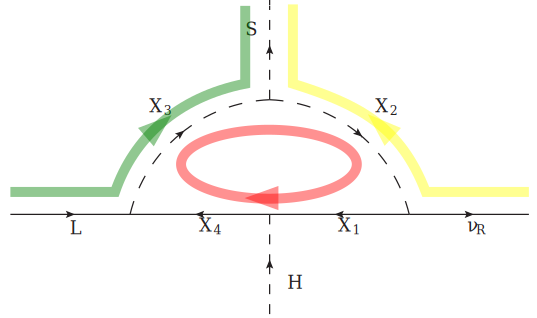
\includegraphics[scale=0.5]{T1-3-D} \hspace{1cm}
  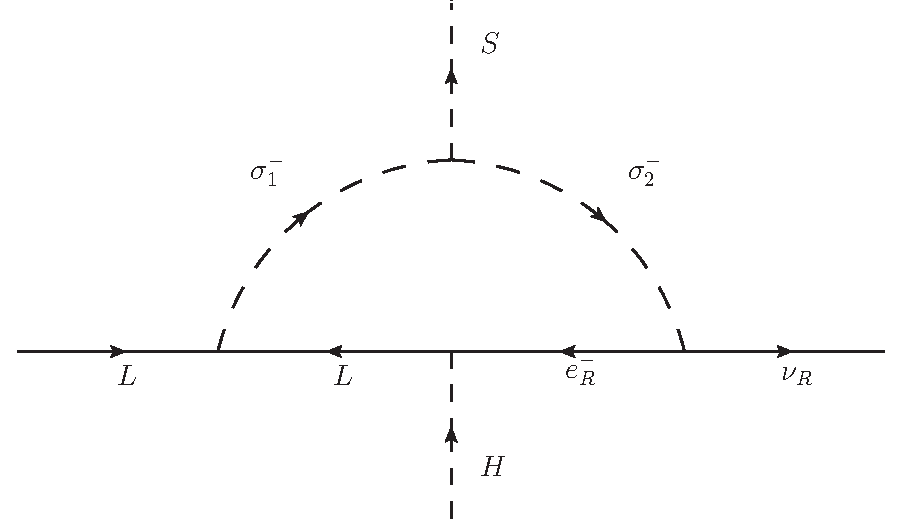
\includegraphics[scale=0.5]{zee}
  \caption{Verde: $L$, amarillo: $\nu_R$, rojo: $X_4$  }
  \label{fig:gg}
\end{figure}
\end{frame}

\begin{frame}[fragile,allowframebreaks]
Para $\operatorname{U(1)}_Y$:
\begin{align}
   \text{(a)}:&\  &-\frac{1}{2}-\frac{1}{2}=&-1 \nonumber\\
   \text{(b)}:&\ &\phantom{-} \frac{1}{2}-1=&-\frac{1}{2} \nonumber\\
  \text{(c)}:&\ &-1=&-1+0  \nonumber\\
  \text{(d)}:&\  & -1=&-1+0  \,.
\end{align}

Para $\operatorname{U}(1)_{B-L}$
\begin{align}
  \text{(a)}:&\  &l +l=&\sigma_1 \nonumber\\
  \text{(b)}:&\  &e+h=&l \nonumber\\
  \text{(c)}:&\  &\sigma_2=&\nu+e \nonumber\\
  \text{(d)}:&\ &\sigma_1=&\sigma_2+s\,.
\end{align}
Combinado con $\operatorname{SU}(2)_L$ y Lorentz
\begin{align}
  \text{(a)}:&\  L_i\cdot L_j \sigma_1^{*} \nonumber\\
  \text{(b)}:&\  \left( e_R \right)^{\dagger} \widetilde{H} \cdot L \nonumber\\
  \text{(c)}:&\  \nu_R e_R^- \sigma_2^+  \nonumber\\
  \text{(d)}:&\ \sigma_1^+\sigma_2^{-} S\,.
\end{align}

La condiciones de consistencia para $\operatorname{U}(1)_{B-L}$ son 
\begin{align}
    \sigma_1=&2l \nonumber\\
  e=&l-h \nonumber\\
  \sigma_2=&\nu+l-h \nonumber\\
  s=&\sigma_1-\sigma_2=2l-\nu-l+h=l-\nu\,.
\end{align}
Con $l=-1$ y $h=0$
\begin{align}
   \sigma_1=&-2 \nonumber\\
    e=&-1 \nonumber\\
\sigma_2=&\nu-1 \nonumber\\
   s=&-1-\nu\,.
\end{align}
Para evitar
\begin{align}
 \left( \nu_R \right)^{\dagger}  L\cdot H\,,\qquad \nu_R \nu_R\,,
\end{align}
requerimos que
\begin{align}
  -\nu -1 +0 \ne& 0\,, & 2 \nu\ne& 0\,.
\end{align}
de modo que
\begin{align}
  \nu\ne& -1,0\,.
\end{align}

A modo de ejemplo,
para $\nu=-4$, entonces $s=3$ y $\sigma_2=-5$ con $\sigma_1=-2$, $l=e=-1$ y $h=0$\,.



  \begin{itemize}
  \item Demuestre que el producto escalar $SU(2)$ entre $L_i$ iguales es cero ($i=1,2$) 
  \item   Establezca las condiciones para que $\sigma_1^-=\sigma_2^-$.
  \end{itemize}

\end{frame}

%\newpage
%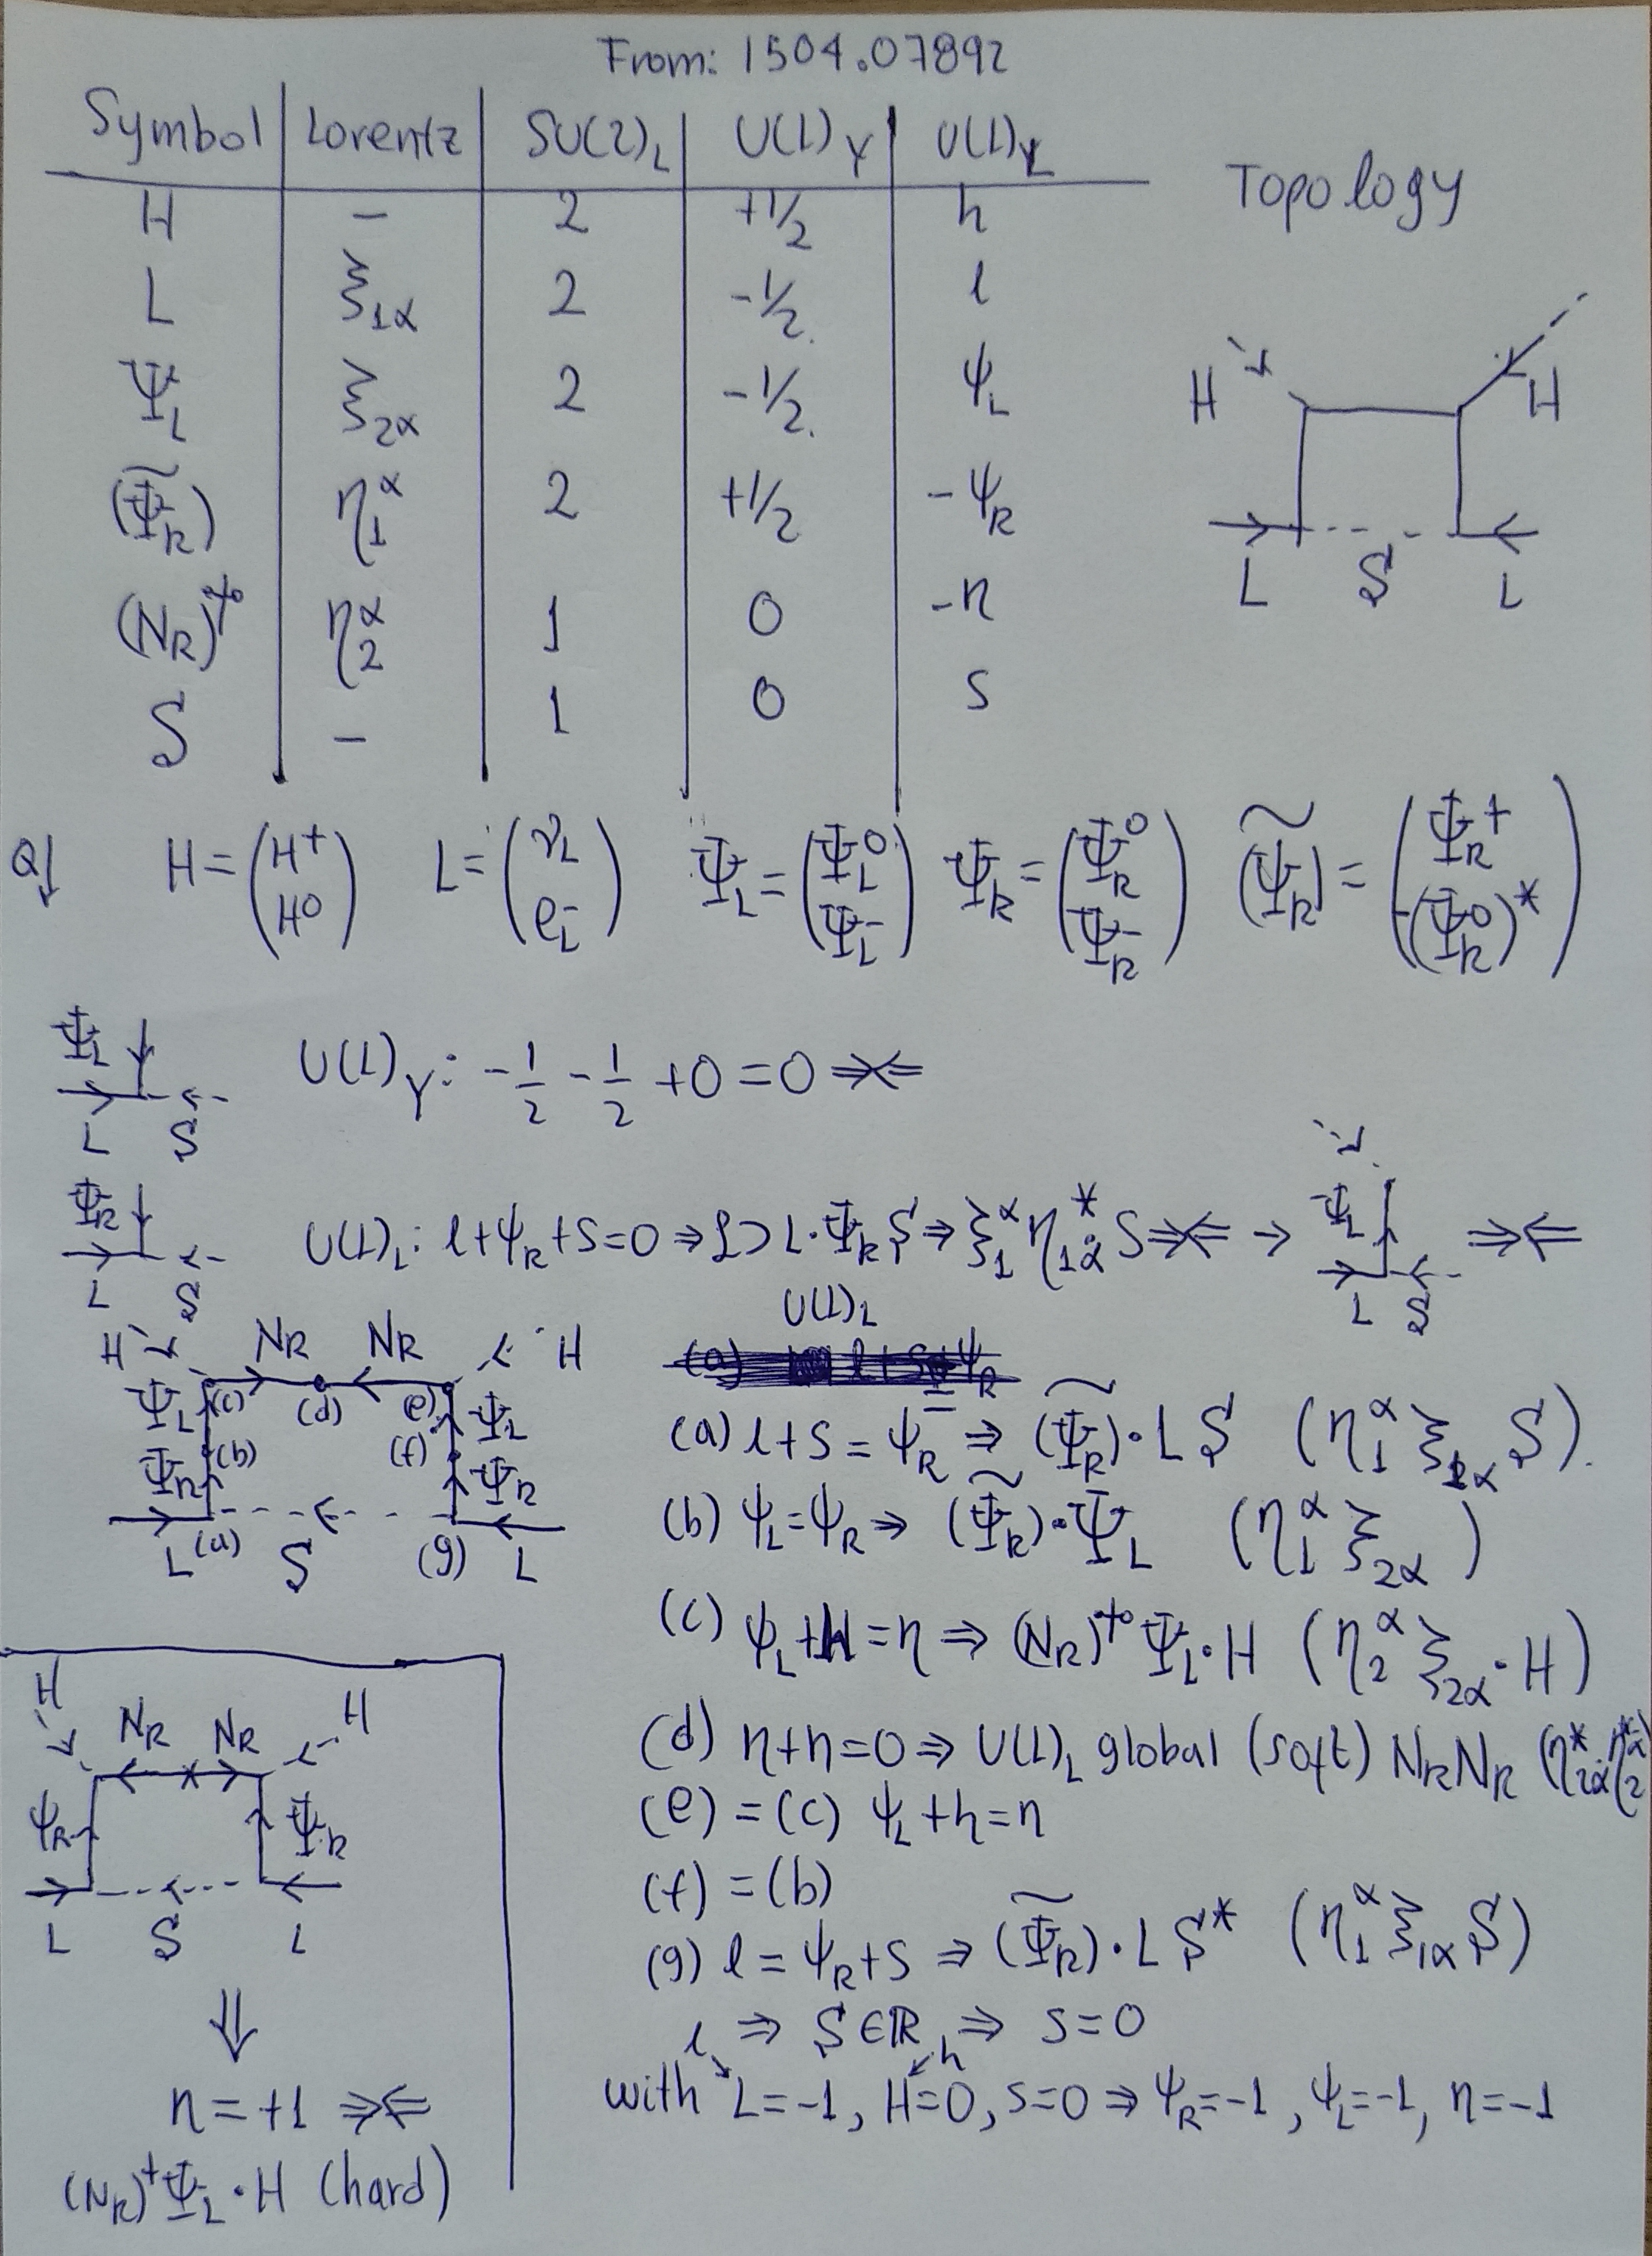
\includegraphics[scale=0.22]{realscalar}

% Para poder considerar el segundo diagrama (en la parte inferior izquierda) debemos hacer $n=0$, de modo que todos los nuevos campos tienen número leptónico cero: $n=\psi_R=\psi_L=s=0$. En ese caso, el único término que viola número leptónico es
% $\widetilde{\left({\Psi}_{R}\right)} \cdot L S$ y por lo tanto las masas de neutrinos deben ser proporcionales al acoplamiento que acompañe a ese término.

\section{Principio de M\'\i nima Acci\'on}
\label{sec:la}

El Principio de Mínima acción establece, una vez fijado el espacio de
coordenadas generalizadas sobre el espacio de configuración, que de
todas las trayectorias posibles que transcurren entre $t_1$ y $t_2$,
el sistema escoger\'a aquella que minimice la acci\'on $S$
\cite{ActionPhysics}.  La magnitud de la acci\'on viene dada para cada
trayectoria por la integral:
\begin{equation}
  \label{eq:la}
   S\left[q_i,\dot{q}_i\right] = \int_{t_{1}}^{t_{2}} L(q_i(t), \dot{q}_i(t),t) dt
\end{equation}
Donde:
$q_i(t)$ son las coordenadas param\'etricas de una trayectoria posible.
$L(q_i,\dot{q}_i,t)$, es la funci\'on lagrangiana del sistema.


Puede probarse mediante principios variacionales, que de todas las trayectorias posibles, la que hace  estacionaria la anterior expresi\'on es la que satisface la siguiente condici\'on $i$:
\begin{equation}
  \label{eq:eel}
 \frac{d}{dt} \left ( \frac{\partial L}{\partial\dot{q}_i} \right ) - \frac{\partial L}{\partial q_i} = 0
\end{equation}
conocidas como las ecuaciones de Euler-Lagrange. La demostraci\'on se
har\'a m\'as adelante para el caso en el que las coordenadas generalizadas
corresponden a funciones de campo. 

De momento mostraremos como la segunda ley de Newton~\cite{NewtonSeconLaw}, puede escribirse en la forma de la ec.~(\ref{eq:eel}).
\begin{align}
\label{eq:fma}
  F&=ma\\
  -\frac{\partial V(x)}{\partial x}&=m\frac{d^2x}{dt^2}\nonumber\\
  &=m\frac{d\dot{x}}{dt}\nonumber\\
  &=\frac{d}{dt}
  \left[
    \frac{\partial}{\partial\dot{x}}
    \left(
      \frac{1}{2}m\dot{x}^2
    \right)
  \right]\nonumber
\end{align}
Podemos introducir el Lagrangiano a cada lado de la igualdad adicionando t\'erminos con la respectiva derivada parcial cero:
\begin{equation*}
  \frac{\partial}{\partial x}
  \left(
\frac{1}{2}m\dot{x}^2-V(x)
  \right)=\frac{d}{dt}
  \left[
    \frac{\partial}{\partial\dot{x}}
    \left(
      \frac{1}{2}m\dot{x}^2-V(x)
    \right)
  \right].
\end{equation*}
Reemplazando $L=\frac{1}{2}m\dot{x}^2-V(x)=T-V$, obtenemos
\begin{equation*}
\frac{d}{dt}\frac{\partial L}{\partial\dot{x}}  -\frac{\partial L}{\partial x}=0.
\end{equation*}
Una forma m\'as rigurosa de escribir la ec.~\eqref{eq:fma} puede encontrarse en~\cite{ActionPhysics}. 

El Hamiltoniano del sistema se obtiene definiendo la variable can\'onica conjugada de $x$
\begin{align}
  p=\frac{\partial L}{\partial\dot{x}}=m \dot{x},
\end{align}
y usando la transformada de Legendre
\begin{align}
  H=p \dot{x}-L=\frac{\partial{L}}{\partial\dot{x}}\dot{x}-L=\frac{1}{2}m\dot{x}^2+V=T+V
\end{align}

Para visualizar el principio de m\'\i nimo de acci\'on se recomienda seguir las actividades del programa interactivo en \texttt{Java} disponible online en \cite{JavaAP}. 
Una versión implementada como Notebook de IPython puede encontrarse aqui: \url{https://github.com/restrepo/ComputationalMethods/blob/master/material/least_action.ipynb}.

Allí se considera el problema de un objeto de 0.2Kg lanzado hacia arriba y retornado al punto de partida 3 segundos despues. Si dividimos la trayectoria en tres intervalos como se muestra en la Fig.~\ref{fig:apple1}, teniendo en cuenta que la velocidad es la pendiente del segmento, para $\Delta t=0.75\,$s $x_1=11.13\,$m, $t_1=0.75\,$s, $x_2=0\,$m, $t_2=1.5\,$s, tenemos que para la trayectoria mostrada
\begin{align}
  S=\int_{t_1}^{t_2}(T-V)dt\approx&\sum_i(T-V)_i\Delta t\nonumber\\
  \approx&\sum_{i=1}^2\left[\frac{1}{2}m\left(\frac{x_i-x_{i-1}}{t_i-t_{i-1}}\right)^2-m g x_i\right]\Delta t\nonumber\\
  \approx&16.67\,\text{J\,s}
\end{align}
\begin{figure}
  \centering
  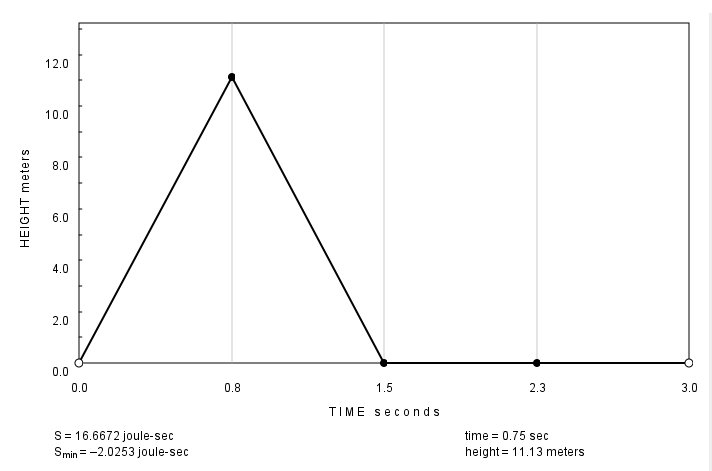
\includegraphics[scale=0.5]{apple1}
  \caption{Ejemplo de c\'alculo de la Acci\'on para una trayectoria arbitraria}
  \label{fig:apple1}
\end{figure}
Iterando el proceso se puede encontrar num\'ericamente (o a mano) la trayectoria que minimiza la acci\'on mostrada en la Fig.~\ref{fig:apple2}
\begin{figure}
  \centering
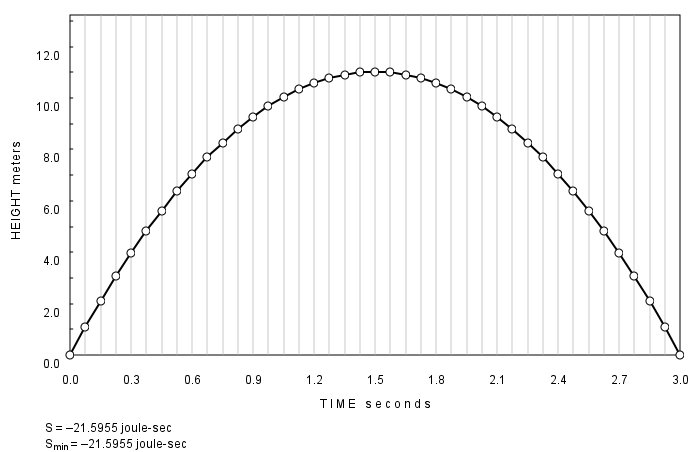
\includegraphics[scale=0.5]{apple2}
  \caption{Trayectoria que minimiza la Acci\'on}
\label{fig:apple2}
\end{figure}
Para una dimensi\'on podemos definir la densidad Lagrangiana como
\begin{equation}
  \mathcal{L}(q,\dot q,t)=\frac{\partial}{\partial q}L(q,\dot q,t)\qquad\text{or}\qquad L(q,\dot q,t)=\int\mathcal{L}(q,\dot q,t)dq.
\end{equation}
La ec.~\eqref{eq:la} puede escribirse entonces como
\begin{equation}
   S\left[q_i,\dot{q}_i\right] = \int \mathcal{L}(q_i(t), \dot{q}_i(t),t)\, dq\,dt.
\end{equation}
Para sistemas continuos es conveniente usar la densidad Lagrangiana. Abordaremos a continuaci\'on el sistema continuo correspondiente a la cuerda cl\'asica unidimensional para construir la densidad Lagrangiana correspondiente. A partir de ella demostraremos las ecuaciones de Euler Lagrange para dicho sistema.

% \left(\right)

\section{De lo Infinitesimal a lo integral}
El método de la Acción es conveniente cuando necesitamos observar de forma integral, es decir, de formal completa. En el caso anterior, la trayectoria completa y sus posibles variaciones.


Es claro que para una problema con modos de oscilación, nos interesa caracterizar el modo de oscilación en su manifestación completa. En la siguiente sección mostraremos las dos formas y veremos que  podremos  estudiar la Acción asociada al modo de oscilación completo.

A nivel física fundamental, sabemos que el objeto físico más importante es el campo, que al igual que un modo de oscilación es un objeto completo que ocupa todo el espacio.
Como resulta que al final las partículas son excitaciones de esos campos, entonces sólo nos tenemos que preocupar de describir los campos y la forma más adecuada es
a través de la Acción.

Para resaltar la importancia de los campos en el mundo subatómico recomendamos la lectura del sigiente artículo y el siguiente video
\begin{itemize}
\item Video en YouTube: \href{kk.org}{
\includegraphics[scale=0.3]{np}}
\item Artículo de divulgación \url{https://www.discovermagazine.com/the-sciences/the-standard-model}
\end{itemize}



\section{La cuerda cl\'asica unidimensional}
\label{sec:la-cuerda-clasica}

\begin{frame}[fragile,allowframebreaks]
Considere una cuerda de longitud $L$ formando un c\'\i rculo de radio $R$.
Es conveniente considerar un conjunto de $N$ part\'\i culas de masa $m$ a
lo largo de la circunferencia, unidas por resortes de longitud $l$ y
constante el\'astica $k$. Los modos vibracionales de la cuerda a lo
largo de la circunferencia se obtienen en l\'\i mite de $N\to\infty$ y $l\to0$ 
%noinstiki

\begin{figure} %noinstiki
  \centering %noinstiki
  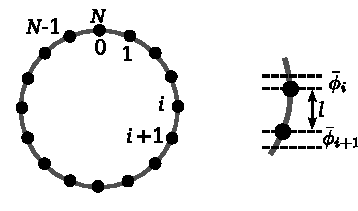
\includegraphics{cuerda} %noinstiki
  \caption{Modelo Cuerda} %noinstiki
  \label{fig:1string} %noinstiki
\end{figure} %noinstiki<div id="fig:1string">Figura cuerda: Modelo cuerda</div>
%noinstiki![cuerda](http://gfif.udea.edu.co/figfs/cuerda.png)
%noinstiki
De acuerdo a la figura 
\ref{fig:1string}, %noinstiki([cuerda](#fig:1string)),
si $\bar{\phi_i}=\bar{\phi}(z_i,t)$ es el
desplazamiento de la $i$--esima masa desde su posici\'on de equilibrio,
entonces el Lagrangiano del sistema de $N$ particulas y resortes es:
\begin{align}
  \label{eq:1strLsum} %noinstiki
  L&=\frac{1}{2}m\sum_{i=0}^{N-1}
  \left(
\frac{\partial\bar\phi_i}{\partial t}
  \right)^2-\frac{1}{2}k\sum_{i=0}^{N-1}
  \left(
\bar\phi_{i+1}-\bar\phi_{i}
  \right)^2,\\
  \label{eq:1strLsumdot} 
&=\frac{1}{2}m\sum_{i=0}^{N-1}
  \left(
    \dot{\bar{\phi_i}}
  \right)^2-\frac{1}{2}k\sum_{i=0}^{N-1}
  \left(
\bar\phi_{i+1}-\bar\phi_{i}
  \right)^2,
\end{align}
donde $\bar\phi_{i+1}-\bar\phi_{i}$ es el desplazamiento relativo entre un par de resortes.
Si $\mu$ es la densidad de la cuerda, $T$ la tensi\'on y $v$ la velocidad, entonces
\begin{align}
  \label{eq:micromacro}
  \mu&=\frac{m}{l}\nonumber\\
  T&=kl\\
  v^2&=\frac{T}{\mu}.\nonumber
\end{align}
(\ref{eq:micromacro})
En el l\'\i mite $l\to0$ y $N\to\infty$, tenemos
\begin{equation}
  \label{eq:barf}
  \bar\phi_i=\bar\phi(z_i,t)\to\bar\phi(z,t),
\end{equation}
que representa la funci\'on de campo del desplazamiento de una masa
infinitesimal de su posici\'on de equilibrio. Entonces
\begin{align}
L&=\frac{1}{2}\sum_{i=0}^{N-1}\frac{m}{l}l
  \left(
    \dot{\bar{\phi_i}}
  \right)^2-\frac{1}{2}\sum_{i=0}^{N-1}(k l) l
  \left(
\frac{\bar\phi_{i+1}-\bar\phi_{i}}{l}
  \right)^2.\nonumber\\
&=\frac{1}{2}\sum_{i=0}^{N-1}\mu
  \left(
    \dot{\bar{\phi_i}}
  \right)^2l-\frac{1}{2}\sum_{i=0}^{N-1}T
  \left(
\frac{\bar\phi_{i+1}-\bar\phi_{i}}{l}
  \right)^2l.
\label{eq:1strLsumm}
\end{align}
En el l\'\i mite continuo $\sum(\cdots)\,l\to\int(\cdots)\,dz$, entonces 
\begin{equation}
\label{eq:238}
  L=\int_0^L\frac{1}{2}
\left[
  \mu\left(\frac{\partial\bar\phi}{\partial t}\right)^2- T\left(\frac{\partial\bar\phi}{\partial z}\right)^2
\right]dz=\int_0^L\mathcal{L}dz,
\end{equation}
con
\begin{equation}
  \label{eq:call1}
  \mathcal{L}=\frac{1}{2}
\left[
  \mu\left(\frac{\partial\bar\phi}{\partial t}\right)^2- T\left(\frac{\partial\bar\phi}{\partial z}\right)^2
\right],
\end{equation}
y
\begin{equation}
  \label{eq:Scall}
  S=\int_{t_1}^{t_2}\int_0^{2\pi R}\mathcal{L}\left( \partial\bar\phi/\partial t,\partial\bar\phi/\partial z
  \right)\,\operatorname{d}t\operatorname{d}z.
\end{equation}
Definiendo
\begin{equation}
  \label{eq:barff}
  \phi=\sqrt{T}\bar\phi,
\end{equation}
tenemos
\begin{align}
  \label{eq:call2}
  \mathcal{L}(\partial\phi/\partial t,\partial\phi/\partial z)=&
\frac{1}{2}
\left[
  \frac{\mu}{T}\left(\frac{\partial\phi}{\partial t}\right)^2- \frac{T}{T}\left(\frac{\partial\phi}{\partial z}\right)^2
\right]\nonumber\\
=&\frac{1}{2}
\left[
  \frac{1}{v^2}\left(\frac{\partial\phi}{\partial t}\right)^2-\left(\frac{\partial\phi}{\partial z}\right)^2
\right],
\end{align}
\end{frame}
Note que:
\begin{align}
  \label{eq:dcalt}
  \frac{\partial}{\partial t}
  \left[
    \frac{\partial\mathcal{L}}{\partial
      (\partial\phi/\partial t)}
  \right]&=    \frac{1}{v^2}\frac{\partial^2\phi}{\partial t^2}\\
  \label{eq:dcalz} %noinstiki
  \frac{\partial}{\partial z}
  \left[
    \frac{\partial\mathcal{L}}{\partial
      (\partial\phi/\partial z)}
  \right]&= -\frac{\partial^2\phi}{\partial z^2}
\end{align}


Si en la ec.~\eqref{eq:1strLsumdot}, tomamos como coordenadas
generalizadas las $N$ $\dot{\bar{\phi_i}}$ y $\bar\phi_i$, entonces, podemos
obtener las ecuaciones de movimiento a partir de las ecuaciones de
Euler-Lagrange \eqref{eq:eel}:
\begin{equation}
  \label{eq:eelfi}
   \frac{d}{dt} \left ( \frac{\partial L}{\partial\dot{\bar{\phi_i}}} \right ) -
   \frac{\partial L}{\partial \bar\phi_i} = 0,
\qquad \text{$i=0$ hasta $N-1$}.
\end{equation}
En el l\'\i mite $l\to0$ y $N\to\infty$, y usando las ecs.~\eqref{eq:dcalt} 
y \eqref{eq:dcalz}, %noinstiki
\begin{align}
  \label{eq:emov1}
  \frac{d}{dt} \left( \frac{\partial L}{\partial\dot{\bar{\phi_i}}} \right)
  &=\frac{d}{dt} \left( m\dot{\bar{\phi_i}} \right)
= m\frac{\partial^2\bar{\phi_i}}{\partial t^2} \nonumber\\
&= T l\left(\frac{\mu}{T}\frac{\partial^2\bar{\phi_i}}{\partial t^2} \right)\nonumber\\
  &\to
  l\sqrt{T}
  \left(
    \frac{1}{v^2}\frac{\partial^2\phi}{\partial t^2}
  \right)\\
  \label{eq:eecalt} %noinstiki
  &=l\sqrt{T}\frac{\partial}{\partial t}
  \left[
    \frac{\partial\mathcal{L}}{\partial
      (\partial\phi/\partial t)}
  \right].
\end{align}
Para el segundo t\'ermino de la ec.~(\ref{eq:eelfi}) n\'otese que
\begin{align}
- \sum_{i=0}^{N-1}\left(\bar\phi_{i+1}-\bar\phi_{i}\right)^2= 
 &-\left(\bar\phi_{1}-\bar\phi_{0}\right)^2-\left(\bar\phi_{2}-\bar\phi_{1}\right)^2-\cdots
-\left(\bar\phi_{(i-1)+1}-\bar\phi_{i-1}\right)^2-\left(\bar\phi_{i+1}-\bar\phi_{i}\right)^2-\cdots\nonumber\\
 =&-\left(\bar\phi_{1}-\bar\phi_{0}\right)^2-\left(\bar\phi_{2}-\bar\phi_{1}\right)^2-\cdots
 -\left(\bar\phi_{i}-\bar\phi_{i-1}\right)^2-\left(\bar\phi_{i+1}-\bar\phi_{i}\right)^2-\cdots\nonumber\\
\end{align}
Entonces
\begin{align}
-\frac{\partial}{\partial\bar\phi_i}  \sum_{i=0}^{N-1}\left(\bar\phi_{i+1}-\bar\phi_{i}\right)^2
=&-2\left(\bar\phi_{i}-\bar\phi_{i-1}\right)-2\left(\bar\phi_{i+1}-\bar\phi_{i}\right)\times(-1)\nonumber\\
=&2l\left[\frac{\bar\phi_{i+1}-\bar\phi_{i}}{l}-\frac{\bar\phi_{i}-\bar\phi_{i-1}}{l}\right].\nonumber
\end{align}
Si $\bar{z}_i$ es el punto medio del intervalo entre $z_{i-1}$ y $z_i$, entonces en el límite de $l\to0$,
\begin{align}
  -\frac{\partial}{\partial\bar\phi_i}  \sum_{i=0}^{N-1}\left(\bar\phi_{i+1}-\bar\phi_{i}\right)^2
  =&2l^2\left\{\frac{[\bar\phi(z_{i+1},t)-\bar\phi(z_{i},t)]/l}{l}-\frac{[\bar\phi(z_{i},t)-\bar\phi(z_{i-1},t)]/l}{l}\right\}\nonumber\\
&2l^2\left[\frac{\partial\bar\phi(\bar z_{i+1},t)/\partial z}{l}-\frac{\partial\bar\phi(\bar z_{i},t)/\partial z}{l}\right]\nonumber\\
  =&2l^2\frac{\partial^2\bar\phi}{\partial z^2}\nonumber\\
  \label{eq:129}
  \to&\frac{2l^2}{\sqrt{T}}\frac{\partial^2\phi}{\partial z^2}.
\end{align}
Usando las ecs.~(\ref{eq:129}) (\ref{eq:micromacro}), tenemos

\begin{align}
  \label{eq:emov2}
  \frac{\partial L}{\partial\bar{\phi_i}}
&=\frac{1}{2}k
\left[-\frac{\partial}{\partial\bar{\phi_i}}\sum_{i=0}^{N-1}\left(\bar\phi_{i+1}-\bar\phi_{i}\right)^2\right]
\nonumber\\
&\to\frac{1}{2}k\left(\frac{2l^2}{\sqrt{T}}\right)\frac{\partial^2\phi}{\partial z^2}
\nonumber\\
&\to  l\sqrt{T}
      \frac{\partial^2\phi}{\partial z^2}\\
  \label{eq:eecalz}
  &=-l\sqrt{T}\frac{\partial}{\partial z}
  \left[
    \frac{\partial\mathcal{L}}{\partial
      (\partial\phi/\partial z)}
  \right].
\end{align}
De las ecuaciones \eqref{eq:emov1} y \eqref{eq:emov2}, obtenemos la
ecuaci\'on de movimiento para el campo $\phi(z,t)$:
\begin{equation}
  \label{eq:econda1}
    \frac{1}{v^2}\frac{\partial^2\phi}{\partial t^2}-\frac{\partial^2\phi}{\partial z^2}=0,
\end{equation}
que corresponde a la ecuaci\'on de onda en una dimensi\'on. En tres
dimensiones obtendr\'\i amos:
\begin{equation}
  \label{eq:econda3}
    \frac{1}{v^2}\frac{\partial^2\phi}{\partial t^2}-\nabla^2\phi=0.
\end{equation}
De otro lado, de las ecuaciones 
\eqref{eq:eecalt} %noinstiki\eqref{eq:emov1}
y \eqref{eq:eecalz}, %noinstiki\eqref{eq:emov2},
obtenemos las ecuaciones de Euler-Lagrange para la densidad Lagrangiana
\begin{equation}
  \label{eq:eelcalls1}
\frac{\partial}{\partial t}
  \left[
    \frac{\partial\mathcal{L}}{\partial
      (\partial\phi/\partial t)}
  \right]+  \frac{\partial}{\partial z}
  \left[
    \frac{\partial\mathcal{L}}{\partial
      (\partial\phi/\partial z)}
  \right]=0.
\end{equation}
En tres dimensiones:
\begin{equation}
  \label{eq:eelcalls1m}
\frac{\partial}{\partial t}
  \left[
    \frac{\partial\mathcal{L}}{\partial
      (\partial\phi/\partial t)}
  \right]+\frac{\partial}{\partial x}
  \left[
    \frac{\partial\mathcal{L}}{\partial
      (\partial\phi/\partial x)}
  \right]+\frac{\partial}{\partial y}
  \left[
    \frac{\partial\mathcal{L}}{\partial
      (\partial\phi/\partial y)}
  \right]+\frac{\partial}{\partial z}
  \left[
    \frac{\partial\mathcal{L}}{\partial
      (\partial\phi/\partial z)}
  \right]=0.
\end{equation}
Definiendo
\begin{equation}
  \label{eq:xmu}
  x^\mu=(x^0,x^i)=(x^0,x^1,x^2,x^3)=(t,x,y,z) \qquad \mu=0,1,2,3,\quad i=1,2,3\,,
\end{equation}
en un sistema de unidades donde $x^0$ tenga las mismas unidades que
$x^i$, podemos expresar las ecuaciones de Euler-Lagrange que satisface
$\mathcal{L}(\partial\phi/\partial x^\mu)$, como
\begin{align*}
 \sum_\mu\frac{\partial}{\partial x^\mu}
  \left[
    \frac{\partial\mathcal{L}}{\partial
      (\partial\phi/\partial x^\mu)}
  \right]&=0\\
 \frac{\partial}{\partial x^\mu}
  \left[
    \frac{\partial\mathcal{L}}{\partial
      (\partial\phi/\partial x^\mu)}
  \right]&=0,
\end{align*}
donde, en la \'ultima ecuaci\'on se ha usado la convenci\'on de suma sobre
\'\i ndices repetidos. 

Si la densidad Lagrangiana depende tambi\'en directamente de $\phi$,
$\mathcal{L}(\partial\phi/\partial x^\mu,\phi)$, entonces la ecuaci\'on de Euler-Lagrange para
las coordenadas generalizadas  $\partial\phi/\partial x^\mu$ y $\phi$, es
\begin{equation}
\label{eq:eelcallf}
 \frac{\partial}{\partial x^\mu}
  \left[
    \frac{\partial\mathcal{L}}{\partial
      (\partial\phi/\partial x^\mu)}
  \right]-\frac{\partial\mathcal{L}}{\partial\phi}=0.
\end{equation}
\'Esta \'ultima ecuaci\'on se deducir\'a usando m\'etodos variacionales en la
secci\'on~\ref{sec:principio-de-minima-call}.

\begin{frame}[fragile,allowframebreaks]
La generalización de la densidad Lagrangiana a tres dimensiones esta dada por
\begin{align}
  \label{eq:dlc3d}
  \mathcal{L}(\partial\phi/\partial t,\partial\phi/\partial x,\partial\phi/\partial y,\partial\phi/\partial z)
=&\frac{1}{2}
\left[
  \frac{1}{v^2}\left(\frac{\partial\phi}{\partial t}\right)^2-\left(\frac{\partial\phi}{\partial x}\right)^2-\left(\frac{\partial\phi}{\partial y}\right)^2-\left(\frac{\partial\phi}{\partial z}\right)^2
\right],
\end{align}
O en forma más compacta, cambiando a un sistema de unidades en el cual $v=1$:
\begin{align}
  \mathcal{L}(\partial_{\mu} \phi)=  \frac{1}{2}{\partial_\mu\phi}\,{\partial^\mu\phi}\,.
\end{align}
Note que para una onda mecánica con velocidad de propagación $v$, la ecuación anterior se usa sólo a modo de notación. Sólo cuando la velocidad de propagación es la velocidad de la luz la densidad Lagrangiana contiene una producto escalar bien definido, el cual es invariante bajo transformaciones de Lorentz. En este caso el producto escalar corresponde al módulo al cuadrado del cuadrivector $\partial_{\mu}\phi$.
\end{frame}

\begin{frame}[fragile,allowframebreaks]
De hecho $\partial_{\mu}$ hace las veces de la coordena generalizada $\dot{q}$ en el Lagrangiano convencional. La coordenada generaliza $q$ para a ser $\phi$ de modo que en general se espera que la densidad Lagrangiana también dependa en $\phi$


\begin{align}
  \label{eq:Lpdp}
  \mathcal{L}(\phi,\partial_{\mu} \phi)=  \frac{1}{2}{\partial_\mu\phi}\,{\partial^\mu\phi}\,.
\end{align}

En tres dimensiones, la densidad Lagrangiana debe ser ahora integrada en un volumen, $V$, para obtener la Lagrangiana
\begin{align}
  L=\int_V \mathcal{L}\left( \phi,\partial_{\mu}\phi \right) \operatorname{d}x\operatorname{d}y\operatorname{d}z\,,
\end{align}
Como $L$ tiene unidades de Energía, en el sistema de unidades naturales las coordenadas tienen unidades de inverso de Energía y por consiguiente la densidad Lagrangiana debe tener unidades de Energía a la cuarta. Finalmente, ya que la cuadridivergencia $\partial_{\mu}=\partial/\partial x^{\mu}$, tiene unidades de Energía, de la ec.~\eqref{eq:Lpdp} podemos concluir entonces que el campo $\phi$,  tiene unidades de Energía:
\begin{align}
 [\mathcal{L}]=E^4 \text{ and } [\partial_{\mu}]=E \to [\phi]=E\,.
\end{align}
La Acción para el campo es entonces
\begin{align}
  S[\phi,\partial_{\mu}\phi]=\int_{t_1}^{t_2} L\left( \phi,\partial_{\mu}\phi \right)=\int_{R} \mathcal{L}\left( \phi,\partial_{\mu}\phi \right) \operatorname{d}t\operatorname{d}x\operatorname{d}y\operatorname{d}z=\int_{R} \mathcal{L}\left( \phi,\partial_{\mu}\phi \right) \operatorname{d}^{4}x\,,
\end{align}
donde los corchete en $S$ significan que la Acción es un \emph{funcional} de las coordenadas generalizadas $\phi,\partial_{\mu}$, $\operatorname{d}^4 x$ es el cuadrivolumen diferencial y $R$ es el cuadrivolumen en el cual se integra la densidad Laggrangiana para obtener la Acción.



\end{frame}



\section{Propiedades de la Acción}


\begin{frame}[fragile,allowframebreaks]
El teorema de Gauss establece que
\begin{equation}
\int_V\boldsymbol{\nabla}\cdot\mathbf{A}\,d^3x=
 \int_S\mathbf{A}\cdot d\mathbf{S}\,.
\end{equation}
Generalizado a cuatro dimensiones, tenemos
\begin{align}
  \label{eq:gauss4d}
\int_{R} \operatorname{d}^4x\,\partial_{\mu} \eta^{\mu}=
\int_{\sigma} \operatorname{d}\sigma_{\mu} \eta^{\mu}\,,   
\end{align}
donde $\mathcal{R}$ es el volumen en cuatro dimensiones (4D) y $\sigma$ la correspondiente hipersuperficie en tres dimensiones.
\end{frame}

Para una densidad Lagrangiana modificada con una derivada total de un cuadrivector
\begin{align}
  \mathcal{L}'=\mathcal{L}+\partial_\mu(\eta^{\mu}(x))
\end{align}
donde $\eta^{\mu}(x)$ es cualquier función de los campos de la densidad Lagrangiana original. Sí asumimos que dichos campos se anulan  sobre la frontera, da lugar a la Acción
\begin{align}
  S'=\int_{R}d^4x\,\mathcal{L}'=&\int_{R}d^4x\,\mathcal{L}+\int_R d^4x\,\partial_\mu\eta^{\mu}\nonumber\\
  =&\int_{R}d^4x\,\mathcal{L}+\int_\sigma \eta^{\mu} d\sigma_{\mu}\nonumber\\
  =&S\,,
\end{align}
para una hipersuperficie suficientemente grande. De modo que dos densidades lagrangianas que difieran solo en derivadas totales dan lugar a la misma Acción. Es claro por ejemplo para el campo electromagnético que su valor se anula a grandes distancias.

\section{Principio de mínima acción}
\label{sec:principio-de-minima-call}


En el Problema variacional de Noether se estudia de forma general como las variaciones de los campos y sus derivadas afectan las leyes de conservación las cuales pueden ser globales o locales. Un sistema binario de estrellas conserva la energía globalmente, pero un sistema binario de estrellas de neutrones donde los efectos relativistas sean importante violan la energía globalmente, es decir, el sistema se vuelve inestable. ¿Qué pasa con la conservación de la energía en ese último caso?



Seguiremos la discusión basada en \cite{Brading:2000hc,Brading:2003nv,Sundermeyer:2014kha}.

\begin{frame}[fragile,allowframebreaks]
%motivar mejor la necesidad de un parámetro de transformación
Estamos interesados en los cambios que sufre la Acción cuando se transforman los campos. Por ejemplo, bajo una transformación de cambio de fase
\begin{align}
  \label{eq:phchg}
  \psi \to \psi'=\operatorname{e}^{i \theta}\psi\,,
\end{align}
si consideremos una transformación de fase pequeña
\begin{align}
  \psi \to \psi'\approx& (1+i\theta)\psi \nonumber\\
                      =&  \psi+i\theta\psi\,.
\end{align} 

Podemos definir el cambio en el campo como
\begin{align}
  \label{eq:deltamatter}
  \delta \psi\equiv \psi'-\psi=&(i\psi) \theta &\to&  & \delta \psi^{*}\equiv \psi^{\prime *}-\psi=&(-i\psi^{*}) \theta \,,
\end{align}
de modo que el cambio en el campo es lineal en el parámetro de la transformación $\theta$.
\end{frame}

\begin{frame}[fragile,allowframebreaks]
De otro lado, cuando se escriben las ecuaciones de Maxwell en términos del cuadrivector de potencial $A^{\mu}(x)$,      estás resultan invariantes bajo la transformación~\eqref{eq:aphicov} (con $\chi\to\theta$)
\begin{align}
  \label{eq:deltarad}
  A^{\mu}(x)\to A^{\prime\mu}(x)= &  A^{\mu}(x) -\partial^{\mu} \theta(x) \nonumber\\
    \delta A^{\mu}(x)\equiv A^{\prime\mu}(x) -A^{\mu}(x)=& -\partial^{\mu} \theta(x)\,.
\end{align}
donde $\theta(x)$ es una función arbitraria que se conoce como parámetro de la transformación. En este caso el cambio del campo va con al cuadriderivada del párametro de la transformación.

La Acción  debe ser también invariante bajo este tipo de transformación, es decir, para el cambio en la Acción
\begin{align}
  \delta S=0\,.
\end{align}
\end{frame}


\begin{frame}[fragile,allowframebreaks]
Para $N$ campos asociados a un parámetro de transformación $\theta$ , la dependencia explicita e implicita de la densidad Lagrangiana da lugar al funcional de Acción
\begin{equation}
  S[\phi_i,\partial_\mu\phi_i;x]=\int_{R}\operatorname{d}^4x\,\mathcal{L}(\phi_i,\partial_\mu\phi_i;x)
\end{equation}


El problema variacional de Noether, que es diferente al principio de Hamilton, puede ser establecido en los siguientes términos:


\noindent
¿Cuales son las condiciones generales que se deben satisfacer para que una dada variación en la variables explícitas e implicitas permitan que la Acción pueda quedar invariante, y de aquí $\delta S=0$, donde $\delta S$ puede o no contener un término de frontera?

Definiendo el cambio interno en el campo como en \eqref{eq:deltaphi}
\begin{align}
  \delta\phi_i(x)=\phi'_i(x)-\phi_i(x)\,,
\end{align}
y el cambio en $x$ bajo una transformación de Lorentz infinitesimal como
\begin{align}
\label{eq:deltax}
  x\to x'=x+\delta x
\end{align}
tenemos que la variación en las variables dependientes e independientes de la Acción son
\begin{align}
   \delta S=&\int_{R}d^4x'\,\mathcal{L} \left( \phi_{i}',\partial_{\mu}\phi'_i;x' \right)- \int_{R}d^4x\,\mathcal{L} \left( \phi_{i}(x),\partial_{\mu}\phi_i(x);x \right) \nonumber\\
     =&\int_{R}\frac{\partial x'}{\partial x}d^4x\,\mathcal{L} \left( \phi_{i}+\delta\phi_i,\partial_{\mu}(\phi_i+\delta\phi_i);x+\delta x \right)- \int_{R}d^4x\,\mathcal{L} \left( \phi_{i},\partial_{\mu}\phi_i;x \right)\,
\end{align}
Derivando \eqref{eq:deltax}, y reemplazadando
\begin{align}
  \frac{\partial x^{\prime \mu}}{\partial x^{\mu}}=1+\partial_{\mu} \left( \delta x^{\mu} \right),
\end{align}
en la expresión anterior, tenemos que
\begin{align}
     \delta S =&\int_{R} \left[ 1+\partial_{\mu} \left( \delta x^{\mu}  \right)\right]  d^4x\,\left\{ \mathcal{L}(\phi_i,\partial_{\mu}\phi_i;x)+\sum_i \left[ \frac{\partial\mathcal{L}}{\partial\phi_i}\delta\phi_{i} +\frac{\partial\mathcal{L}}{\partial(\partial_{\mu}\phi_i)}\partial_{\mu}(\delta\phi_{i}) \right]+\left( \partial_{\mu}\mathcal{L} \right)\delta x^{\mu} \right\}\nonumber\\
      &- \int_{R}d^4x\,\mathcal{L} \left( \phi_{i},\partial_{\mu}\phi_i;x \right) \nonumber\\
     =&\int_{R} d^4x\,\left[ \partial_{\mu} \left( \delta x^{\mu}  \right)\right] \mathcal{L} + \int_{R}d^4x\,\left\{\sum_i \left[ \frac{\partial\mathcal{L}}{\partial\phi_i}\delta\phi_{i} +\frac{\partial\mathcal{L}}{\partial(\partial_{\mu}\phi_i)}\partial_{\mu}(\delta\phi_{i}) \right]+\left( \partial_{\mu}\mathcal{L} \right)\delta x^{\mu} \right\}+\mathcal{O} \left( \delta^2 \right)\nonumber\\
     \approx&\int_{R} d^4x\,\partial_{\mu} \left(\mathcal{L} \delta x^{\mu}  \right)  + \int_{R}d^4x\,\sum_i \left\{ \frac{\partial\mathcal{L}}{\partial\phi_i}\delta\phi_{i} +\partial_{\mu} \left[ \frac{\partial\mathcal{L}}{\partial(\partial_{\mu}\phi_i)}\delta\phi_{i} \right]-\partial_{\mu} \left[ \frac{\partial\mathcal{L}}{\partial(\partial_{\mu}\phi_i)}\right]\delta\phi_{i}  \right\}\,,
\end{align}
y reordenando los términos con derivada total
\begin{align}
  \delta S =&
\int_{R} d^4x\,\partial_{\mu} \left[\mathcal{L} \delta x^{\mu} + \frac{\partial\mathcal{L}}{\partial(\partial_{\mu}\phi_i)}\delta\phi_{i} \right]  + \int_{R}d^4x\,\sum_i \left\{ \frac{\partial\mathcal{L}}{\partial\phi_i} -\partial_{\mu} \left[ \frac{\partial\mathcal{L}}{\partial(\partial_{\mu}\phi_i)}\right]  \right\}\delta\phi_{i}\,,              
\end{align}
\end{frame}

\begin{frame}[fragile,allowframebreaks]
La condición $\delta S=0$ implica que
\begin{align}
\label{eq:masterint}
\int_R \operatorname{d}^4x  \sum_i \mathcal{E}_i \delta\phi_i =\int_R \operatorname{d}^4x  \partial_{\mu} B^{\mu}\,,
\end{align}
donde
\begin{align}
\label{eq:master2}
  \mathcal{E}_i=&\partial_{\mu} \left[ \frac{\partial\mathcal{L}}{\partial(\partial_{\mu}\phi_i)}\right]-\frac{\partial\mathcal{L}}{\partial\phi_i} & B^{\mu}=\mathcal{L} \delta x^{\mu} +\sum_i \frac{\partial\mathcal{L}}{\partial(\partial_{\mu}\phi_i)}\delta\phi_{i}\,. 
\end{align}
\end{frame}


\section{Ecuaciones de Euler-Lagrange}
%% TODO: Mejorar


Aplicando las condiciones de Frontera usando  el teorema de Gauss en 4D dado en la ec.~\eqref{eq:gauss4d} en el lado derecho de \eqref{eq:masterint}
\begin{align}
\int_R \operatorname{d}^4x  \sum_i \mathcal{E}_i \delta\phi_i =\int_\sigma \operatorname{d}^4x \,, B^{\mu}\operatorname{d}\sigma_{\mu}\,,
\end{align}
de modo que la función de los campos $B^{\mu}(\phi_i,\partial_{\mu} \phi_{i})$ está evaluada sobre la frontera.
Es claro que la integral de frontera se anula si imponemos que la variación tanto de la coordenadas, $\delta x^{\mu}$, como de los campos, $\delta \phi_{i}$ , en la frontera se hagan cero. Esto es equivalente a la anulación de las trayectorias en los extremos para la Acción en mecánica clásica, 
% Para un volumen suficientemente grande, si los campos se anulan en la frontera, como los campos electromagnéticos que se,
entonces la integral del lado derecho se anula 
\begin{align}
\int_R \operatorname{d}^4x  \sum_i \mathcal{E}_i \delta\phi_i =0
\end{align}
Como $\delta\phi_i$ es arbitrario, lo que se debe anular es $\mathcal{E}_i$ para cada $i$.

\begin{frame}[fragile,allowframebreaks]
Obtenemos entonces las ecuaciones de Euler-Lagrange para cada campo $\phi_i$
\begin{align}
\label{eq:eelcallfmu}
  \partial_{\mu} \left[ \frac{\partial\mathcal{L}}{\partial(\partial_{\mu}\phi_i)}\right]-\frac{\partial\mathcal{L}}{\partial\phi_i}=0
\end{align}

La misma condición de nulidad de los campos en la frontera permite establecer que 
\end{frame}

Usando el principio de m\'\i nima acci\'on en t\'erminos del campo $\phi$, tenemos que para la densidad Lagrangiana~\eqref{eq:call2}
\begin{align}
  \mathcal{L}=&\frac{1}{2}  \left[
  \frac{1}{v^2}\left(\frac{\partial\phi}{\partial t}\right)^2-\left(\frac{\partial\phi}{\partial z}\right)^2
\right],
\end{align}
las ecuaciones de Euler-Lagrange~\eqref{eq:eelcallfmu}
\begin{align}
  \partial_0\left[\frac{\partial\mathcal{L}}{\partial(\partial_0\phi)}\right]+
\partial_3\left[\frac{\partial\mathcal{L}}{\partial(\partial_3\phi)}\right]
-\frac{\partial\mathcal{L}}{\partial\phi}=&0\nonumber\\
  \frac{\partial}{\partial t}\left[\frac{\partial\mathcal{L}}{\partial(\partial\phi/\partial t)}\right]+
\frac{\partial}{\partial z}\left[\frac{\partial\mathcal{L}}{\partial(\partial\phi/\partial z)}\right]
=&0\nonumber\\
 \frac{1}{v^2}\frac{\partial}{\partial t}\left[\frac{\partial\phi}{\partial t}\right]
-\frac{\partial}{\partial z}\left[\frac{\partial\phi}{\partial z}\right]=&0\nonumber\\
 \frac{1}{v^2}\frac{\partial^2\phi}{\partial t^2}-\frac{\partial^2\phi}{\partial z^2}=&0\,,
\end{align}
que corresponde a la ec.~\eqref{eq:econda1}.


Generalizando a tres dimensiones vemos que la ecuación de Euler-Lagrange para la
\begin{frame}[fragile,allowframebreaks]
densidad Lagrangiana de una onda propagandose a una velocidad $v$, eq.~\eqref{eq:econda3},
\begin{align}
  \mathcal{L}(\partial_{\mu} \phi)=  \frac{1}{2}{\partial_\mu\phi}\,{\partial^\mu\phi}
  =& \frac{1}{2}g^{\mu\nu}{\partial_\mu\phi}\,{\partial_{\nu}\phi}\,,
\end{align}
\end{frame}
se puede calcular a partir de
\begin{align}
  \frac{\partial\mathcal{L}}{\partial(\partial_{\sigma}\phi)}=&
                                                                \frac{\partial}{\partial(\partial_{\sigma}\phi)} \left( \frac{1}{2}g^{\mu\nu}{\partial_\mu\phi}\,{\partial_{\nu}\phi} \right) \nonumber\\
    =&\frac{1}{2} \left\{  g^{\mu\nu}\left[ \frac{\partial \left( \partial_{\mu}\phi \right)}{\partial \left( \partial_{\sigma}\phi \right)} \right]\partial_{\nu}\phi
     +g^{\mu\nu} \partial_{\mu}\phi \left[ \frac{\partial \left( \partial_{\nu}\phi \right)}{\partial \left( \partial_{\sigma}\phi \right)} \right] \right\} \nonumber\\
    =&\frac{1}{2}\left(  g^{\mu\nu}\delta^{\sigma}_{\mu}\partial_{\nu}\phi
     +  g^{\mu\nu}\partial_{\mu}\phi \delta ^{\sigma}_{\nu}\right) \nonumber\\
    =&\frac{1}{2}\left(  g^{\sigma\nu}\partial_{\nu}\phi
       +  g^{\mu\sigma}\partial_{\mu}\phi \right) \nonumber\\
           =&\frac{1}{2}\left(  \partial^{\sigma}\phi
     + \partial^{\sigma}\phi \right) \nonumber\\
=& \partial^{\sigma}\phi\,.
\end{align}
De modo que
\begin{align}
   \partial_{\sigma} \left[ \frac{\partial\mathcal{L}}{\partial(\partial_{\sigma}\phi)}\right]-\frac{\partial\mathcal{L}}{\partial\phi}=&0 \nonumber\\
  \partial_{\sigma} \left[ \frac{\partial\mathcal{L}}{\partial(\partial_{\sigma}\phi)}\right]=&0 \nonumber\\
       \partial_{\sigma}\partial^{\sigma}\phi=&0 \,.
\end{align}
\begin{frame}[fragile,allowframebreaks]
Teniendo en cuenta que $\sigma$ es un índice modo, podemos escribir la ecuación de onda en la forma conocida:
\begin{align}
     \partial_{\mu}\partial^{\mu}\phi=&0 \nonumber\\
     \frac{1}{v^2}\frac{\partial^2\phi}{\partial t^2}-\nabla^2\phi=&0\,.
\end{align}
\end{frame}

\textbf{Ejercicio:} Demuestre que la ecuación de Klein-Gordon en \eqref{eq:KG} proviende de una densidad Lagragiana del tipo
\begin{align}
  \mathcal{L}(\phi,\partial_{\mu} \phi)=  \frac{1}{2}{\partial_\mu\phi}\,{\partial^\mu\phi}-V(\phi)\,,
\end{align}
donde
\begin{align}
  V(\phi)=\frac{1}{2}m^2 \phi^2\,.
\end{align}

En el ejercicio anterio el gráfico del \emph{potencial} escalar $V(\phi)$ corresponde a la parábola mostrada en la figura~\ref{fig:x2ini}


\begin{figure} %noinstiki
  \centering %noinstiki
  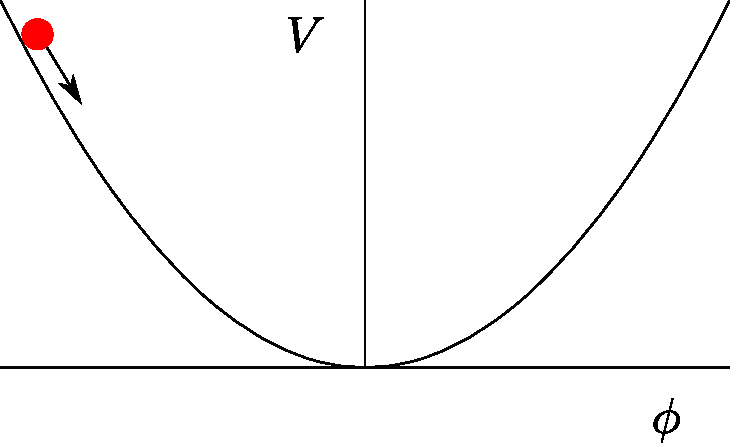
\includegraphics[scale=0.8]{vphi2roll}
  \caption{$V(\phi)=\frac{1}{2}m^2 \phi^2$ con $m^2\gt 0$} %noinstiki
  \label{fig:x2ini} %noinstiki
\end{figure} %n


La interpretación tomada de la teoría cuántica de campos completa, nos permite visualizar la excitación del campo como una partícula rodando a través de las paredes del potencial como se muestra en la figrua. La masa del campo corresponde a las oscilaciones alrededor del mínimo que suben las parades y que por consiguiente \emph{cuestan energía}. Esta interpretación la usaremos en el Capítulo~\ref{rupt-espont-de} para enteder el mecánismo de Higgs.

El potencial escalar se puede modelar para que el campo escalar $\phi$ pueda interpretarse por ejemplo como el inflatón en el Universo primitivo. Mientras la partícula rueda hacía el mínimo el Universo sufre una expansión exponencial y cuando termina oscilando alrededor del mismo el universo sufre una fase de \emph{recalentamiento} mediante la cual la energía del inflaton genera todas las partículas y antipartículas del modelo estándar en cantidades de $10^{90}$. La radiación cósmica de fondo esta compuesta de esos $10^{90}$ fotones de primigéneos y las anisotropías observadas en ella proviened de las fluctuaciones cuánticas del inflaton magnificadas por la expansión exponencial.

\begin{frame}[fragile,allowframebreaks]
\textbf{Ejercicio:}
\begin{enumerate}
\item  Demuestre que los terminos con derivada de la densidad Lagrangiana para un campo escalar complejo
\begin{align}
  \phi\equiv&\frac{\phi_1+i\phi_2}{\sqrt{2}} &\to&&   \phi^{*}=&\frac{\phi_1-i\phi_2}{\sqrt{2}}\,,
\end{align}
que sea invariante bajo el Grupo $U(1)$ de sus cambios de fase~\eqref{eq:phchg}, se puede escribir de forma única como
\begin{align}
  \mathcal{L}(\partial_{\mu} \phi,\partial_{\mu} \phi^{*})=  {\partial_\mu\phi^{*}}\,{\partial^\mu\phi}=\frac{1}{2}\partial_{\mu}\phi_1 \partial^{\mu}\phi_1+\frac{1}{2}\partial_{\mu}\phi_2 \partial^{\mu}\phi_2\,,
\end{align}
es decir, como la suma de la densidad Lagrangiana para dos campos reales independientes.
\item Cambiando a las variables generalizadas $\phi_1\to \phi$, $\phi_2\to \phi^{*}$, encuentre las ecuaciones de Euler Lagrange para $\phi$ y $\phi^{*}$
\end{enumerate}
\end{frame}



%%Radical view:
% 1) Transformaciones externas
% 2) Transformaciones internas

% 1) Transformaciones externas

\section{Ecuación de continuidad}
\begin{frame}[fragile,allowframebreaks]
Las transformaciones que bajo algunas condiciones dejan invariante a la acción, van a estar relacionadas con cargas conservadas. A continuación definiremos con un ejemplo conocido que es una carga conservada.

Para entender el significado físico de la ecuación de continuidad consideremos una cuadri-corriente asociada por ejemplo a la densidad de carga y corriente eléctricas. Expandiendo la ecuación de continuidad en sus componentes espaciales y temporales tenemos que
\begin{align}
  \partial_\mu j^\mu=&0&\nonumber\\
  \partial_0 j^0+ \partial_i j^i=&0\,,&\text{suma sobre $i$}\nonumber\\
  \frac{\partial j^0}{\partial t}+ \boldsymbol{\nabla}\cdot\boldsymbol{j}=&0\,.
\end{align}
Integrando sobre el volumen y aplicando el teorema de Gauss
\begin{align}
  \int_V \operatorname{d}^3x\,\frac{\partial j^0}{\partial t}
+\int_S \boldsymbol{j}\cdot \operatorname{d}  \boldsymbol{S}=&0\,.
\end{align}
Si interpretamos $j^0$ como la densidad, $\rho$, de una cierta carga $Q$, tal que
\begin{align}
  Q=\int_{V} \operatorname{d}^3x\, j^0= \int_{V} \operatorname{d}^3x\, \rho\,,
\end{align}
entonces, si escogemos $S$ como una superficie suficientemente grande para contener toda la distribución de carga $Q$ en su interior, tendremos que la integral sobre la superficie se anula
\begin{align}
  \int_S \boldsymbol{j}\cdot \operatorname{d} \boldsymbol{S}=&0\,,
\end{align}
y por consiguiente
\begin{align}
  \int_V \operatorname{d}^3x\,\frac{\partial j^0}{\partial t}=&
\frac{\operatorname{d}}{\operatorname{d}t}\int_V \operatorname{d}^3x\,\rho \nonumber\\
=&\frac{\operatorname{d}Q}{\operatorname{d}t}\nonumber\\
  =&0\,.
\end{align}
Es decir, que la carga es independiente del tiempo, y por lo tanto se conserva.
\end{frame}



\section{Tranformaciones externas}
\label{sec:tranf-extern}
\begin{frame}[fragile,allowframebreaks]
Un desplazamiento infinitesimal, que equivale a repeterir un experimento en laboratorio desplazado en el tiempo o en el espacio,
puede parametrizarse sin perdida de generalidad como
\begin{align}
  x^\mu\to{x'}^\mu=&x^\mu+\delta x^{\mu}\,.
\end{align}

Para visualizar más fácilmente la situación para un campo escalar, supongamos de momento que $\delta x^{\mu}$ corresponde  traslaci\'on espacio--temporal.

Tenemos
\begin{align}
  \phi'(x')&=\phi'(x+\delta x)\\
  &\approx\phi'(x)+\frac{\partial\phi'(x)}{\partial x^\mu}\delta x^\mu\\
  &=[\phi(x)+\delta\phi(x)]+\frac{\partial}{\partial x^\mu}[\phi(x)+\delta\phi(x)]\delta x^\mu\\
  &\approx\phi(x)+\delta\phi(x)+\frac{\partial\phi(x)}{\partial x^\mu}\delta x^\mu,
\end{align}
donde, por simplicidad, $\phi$ es un campo real. Entonces,
\begin{equation}
  \label{eq:Deltaf}
  \Delta\phi(x)\equiv\phi'(x')-\phi(x)=\delta\phi(x)+\frac{\partial\phi(x)}{\partial x^\mu}\delta x^\mu.
\end{equation}
Para una traslaci\'on, $\Delta\phi(x)=0$, ver figura 
\ref{fig:trasla}. %noinstiki([trasla](#fig:trasla)).
De modo que
\begin{equation}
  \label{eq:dmuxmu}
  \delta\phi=-(\partial_\mu\phi)\delta x^\mu,
\end{equation}
y la transformaci\'on del campo $\phi$ como consecuencia de la traslaci\'on es
\begin{align}
  \phi(x)\to\phi'(x)=\phi(x)-\delta\phi(x)=\phi(x)+(\partial_\mu\phi(x))\delta x^\mu\,.
\end{align}
%noinstiki

\begin{figure} %noinstiki
  \centering %noinstiki
  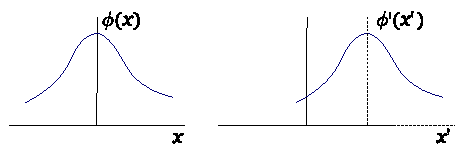
\includegraphics{trasla} %noinstiki
  \caption{Traslaci\'on de funci\'on y coordenadas en una dimensi\'on: $\phi(x)=\phi'(x')$ } %noinstiki
  \label{fig:trasla} %noinstiki
\end{figure} %noinstiki<div id="fig:trasla">Figura trasla:Traslaci\'on de funci\'on y coordenadas $\phi(x)=\phi(x')$ </div>
%noinstiki![trasla](http://gfif.udea.edu.co/figfs/trasla.png)
%noinstiki

\end{frame}




\section{Primer teorema de Noether para simetrías externas}
El primer teorema de Noether surge al asumir que
\begin{itemize}
\item Los parámetros de transformación son globales, es decir, que los parámetros de la transformación no dependen del punto del espacio tiempo.
\item El conjunto de campos satisface las ecuaciones de Euler-Lagrange.
\end{itemize}

Por consiguiente, la ecuación~\eqref{eq:masterint} se reduce a
\begin{align}
\int_R \operatorname{d}^4x \, \partial_{\mu} B^{\mu}=0\,.
\end{align}
Por lo tanto:

\subsubsection{Teorema 1}
Por  cada parámetro asociado a una transformación global  existe una ecuación de continuidad del tipo
\begin{align}
  \label{eq:dmubmu}
   \partial_{\mu} B^{\mu}=0\,,
\end{align}
con $B^{\mu}$ dado por la ecuación~\eqref{eq:master2}.

\begin{frame}[fragile,allowframebreaks]
  Consideremos el caso en el cual el campo es sólo afectado en su dependencia espacio-temporal. Como ocurre para una la transformación externa de traslación global
  discutida en la Sección~\ref{sec:tranf-extern}. Allí, un desplazamiento constante
\begin{align}
  x^\mu\to{x'}^\mu=&x^\mu+\delta x^{\mu}\,,
\end{align}
ocasiona un cambio en
  un campo escalar de Lorentz dado por la ec.~\eqref{eq:dmuxmu}
  \begin{align}
    \delta\phi_{i}=-\left( \partial_{\nu}\phi_i \right)\delta x^{\nu}\,.
  \end{align}

  De acuerdo al Teorema 1 de Noether, los cuatro posibles parámetros de desplazamiento deben dar lugar a cuatro ecuaciones de continuidad para (suma sobre indices repetidos)
\begin{align}
     B^{\mu}=& \mathcal{L} \delta x^{\mu} + \frac{\partial\mathcal{L}}{\partial(\partial_{\mu}\phi_i)}\delta\phi_{i} \nonumber\\
  =&\delta_{\nu}^{\mu} \mathcal{L} \delta x^{\nu} - \frac{\partial\mathcal{L}}{\partial(\partial_{\mu}\phi_i)} \left( \partial_{\nu}\phi_i \right)\delta x^{\nu}   \nonumber\\
  =&- \left[\frac{\partial\mathcal{L}}{\partial(\partial_{\mu}\phi_i)} \left( \partial_{\nu}\phi_i \right) - \delta_{\nu}^{\mu} \mathcal{L} \right] \delta x^{\nu}   \nonumber\\
  =&    - T^{\mu}_{\nu} \delta x^{\nu}\,,
\end{align}
donde, hemos definido
\begin{align}
  T^{\mu}_{\nu}\equiv\sum_i \frac{\partial\mathcal{L}}{\partial(\partial_{\mu}\phi_i)}\partial_{\nu}\phi_i-\delta^{\mu}_{\nu}\mathcal{L}
\end{align}
si los campos $\phi_{i}$ satisfacen la ecuaciones de Euler-Lagrange, $\mathcal{E}_i=0\,$, tenemos que
\begin{align}
  \partial_{\mu} \left( T^{\mu}_{\nu} \delta x^{\nu}\right)=0\,.
\end{align}
Si $\delta x^{\nu}$ es constante, como se espera en el caso de sistemas inerciales, se satisfacen las cuatro  ecuaciones de continuidad (una para cada $\nu$)
\begin{align}
  \partial_{\mu} T^{\mu}_{\nu}=0\,.
\end{align}
El tensor $T^\mu_\nu$ proviene de asumir la homogeneidad del espacio y el tiempo y es llamado el tensor de momentum--energía. 
La densidad Hamiltonina se obtiene de $T^0_0$
\begin{align}
  \label{eq:3}
\mathcal{H}&=T^0_0=\frac{\partial\mathcal{L}}{\partial\dot{\phi}}\dot{\phi}
      -\mathcal{L}\\
      &=\pi(x)\frac{\partial\phi(x)}{\partial t}-\mathcal{L}.
\end{align}
Comparando con la expresi\'on correspondiente en la formulaci\'on
Lagrangiana de la Mec\'anica Cl\'asica, tenemos que si $\phi(x)$ es la
variable can\'onica, la variable can\'onica conjugada es $\pi(x)$
\begin{equation}
  \label{eq:4}
  \pi(x)=\frac{\partial\mathcal{L}}{\partial(\partial\phi(x)/\partial t)}.
\end{equation}
El teorema de Noether en este caso establece que la invarianza de la Acci\'on bajo traslaciones temporales da lugar a la ecuación de continuidad (\ref{eq:ecncontiJ}) para $\nu=0$
\begin{align}
\label{eq:122}
  \partial_\mu T^\mu_0=0
\end{align}
cuya carga conservada corresponde a la energía
\begin{align}
  H=\int_V d^3x\, T^0_0=\int_V d^3x\,\mathcal{H}.
\end{align}
De igual forma la invarianza bajo traslaciones espaciales de lugar a ecuaciones de continuidad para cada componente $\nu=i$
 ($i=1,2,3$)
 \begin{align}
   \label{eq:235}
   \partial_\mu T^\mu_i=0,
 \end{align}
cuyas densidad de cargas conservadas, $T^0_i$, que en forma vectorial escribiremos como $\mathbf{T}^0$, dan lugar a la conservaci\'on del momentum
\begin{align}
  \mathbf{P}=\int_V d^3x\,\mathbf{T}^0\,.
\end{align}
Generalizando a un campo complejo
\begin{equation}
  \label{eq:138}
     T^\mu_\nu=\frac{\partial\mathcal{L}}{\partial(\partial_\mu\phi)}(\partial_\nu\phi)+(\partial_\nu\phi^*)\frac{\partial\mathcal{L}}{\partial(\partial_\mu\phi^*)}
      -\delta^\mu_\nu\mathcal{L}
\end{equation}

\end{frame}



% \subsection{Teorema de Noether para simetr\'\i as externas}

% Si $a^\mu$ es constante (un an\'alisis m\'as general es hecho en \cite{r})
% \begin{equation}
%   d^4x'=d^4x
% \end{equation}
% En este caso, asumiendo que el campo satisface las ecuaciones de
% Euler-Lagrange y usando la ec.~\eqref{eq:dmuxmu} y (\ref{eq:eelcallfmu}) tenemos
% \begin{align}
%   \delta S&=\int_{R}d^4x\,\mathcal{L}(\phi',\partial_\mu\phi',x')-\int_{R}d^4x\,\mathcal{L}(\phi(x),\partial_\mu\phi(x),x)\nonumber\\
%   &=\int_{R}d^4x\,\mathcal{L}(\phi+\delta\phi,\partial_\mu\phi+\partial_\mu(\delta\phi),x+\delta a)-\int_{R}d^4x\,\mathcal{L}\nonumber\\
%   &\approx\int_{R}d^4x\,
%   \left[\mathcal{L}+
%     \frac{\partial\mathcal{L}}{\partial\phi}\delta\phi+\frac{\partial\mathcal{L}}{\partial(\partial_\mu\phi)}\partial_\mu(\delta\phi)+
%     (\partial_\mu\mathcal{L})\delta a^\mu\right]-\int_{R}d^4x\,\mathcal{L}\nonumber\\
%   &=\int_{R}d^4x\,
%   \left[
%     \frac{\partial\mathcal{L}}{\partial\phi}\delta\phi+\frac{\partial\mathcal{L}}{\partial(\partial_\mu\phi)}\partial_\mu(\delta\phi)+
%     (\partial_\mu\mathcal{L})\delta a^\mu\right]\nonumber\\
%   &=\int_{R}d^4x\,
%   \left\{ 
%     \left[\partial_\mu\left(\frac{\partial\mathcal{L}}{\partial(\partial_\mu\phi)}
%     \right)\right]\delta\phi+\frac{\partial\mathcal{L}}{\partial(\partial_\mu\phi)}\partial_\mu(\delta\phi)+
%     (\partial_\mu\mathcal{L})\delta a^\mu\right\}\nonumber\\
%   &=\int_{R}d^4x\left\{ 
%     \partial_\mu\left[\frac{\partial\mathcal{L}}{\partial(\partial_\mu\phi)}\delta\phi\right]
%   +(\partial_\mu\mathcal{L})\delta a^\mu\right\}\nonumber\\
%   &=\int_{R}d^4x\,
%     \partial_\mu\left[
%       -\frac{\partial\mathcal{L}}{\partial(\partial_\mu\phi)}(\partial_\nu\phi)
%       +\delta^\mu_\nu\mathcal{L}
%     \right]\delta a^\nu\nonumber\\
%     \label{eq:2}
%   &=\int_{R}d^4x\,
%   \left(
%     \partial_\mu T^\mu_\nu
%   \right)\delta a^\nu=0.
% \end{align}



\section{Transformaciones internas}

Una consecuencia del primer teorema de Noether es que por cada simetría global de la Acción existe una carga conservada. 




La virtud del trabajo de Noether~\cite{Noether,Brading:2000hc,Brading:2003nv,Sundermeyer:2014kha} fue separar los resultados  en los casos de grupos de simetrías globales en los cuales el parámetro de transformación no depende del punto del espacio tiempo (como es el caso de las transformaciones a velocidad constante la relatividad especial: $v=\text{cte}$) del caso en que los grupos de simetría dependan del punto del espacio-tiempo (como los sistemas acelerados de la relatividad general donde la velocidad depende el punto del espacio-tiempo: $v(x)$).

En el caso de teorías de campos, estamos más interesados en simetría de espacios internos como puede ser el cambio de fase de la función de onda en la ecuación de Schrödinger. Un cambio de fase, $\theta$, es un caso particular del parámetro de la transformación. En general el parámetro de una transformación interna puede ser constante, $\theta=\text{cte}$, que corresponde a una transformación de fase  \emph{global}, o depender del punto del espacio tiempo, $\theta(x)$, que corresponde  a una transformación  de fase \emph{local}. Las simetrías internas estan caracterizadas por la condición $\delta x^\mu=0$ 

Nos enfocaremos en esta sección en la formulación de los dos teoremas de Noether para el caso de simetrías internas globales y locales.   


Si la transformación depende de algún parámetro $\theta$ continuo, entonces podemos garantizar la existencia de un parámetro infinitesimal tal que
\begin{align}
\label{eq:infdt}
 \delta\phi_i= a_{i}\left( \phi_{i},\partial_{\mu}\phi_{i} \right) \theta(x)+b^{\nu}_i \left( \phi_{i},\partial_{\mu}\phi_{i} \right) \partial_{\nu}\theta(x)\,,
\end{align}

Para concretar, consideremos como transformación interna el cambio de fase de una función compleja
\begin{align}
  \phi\to \phi'=\operatorname{e}^{i\theta}\phi\,.
\end{align}
Para el cambio infinitesimal del campo y su complejo conjugado,  haciendo $\phi_1=\phi$ y $\phi_2=\phi^{*}$ y
para un $\theta$ suficientemente pequeño, obtenemos~\eqref{eq:deltamatter}
\begin{align}
  \delta\phi=&a_1 \theta\,, &  \delta\phi^{*}=&  a_2 \theta\,, 
\end{align}
donde
\begin{align}
  \label{eq:ai}
  a_1=& i\phi \,, & a_2=&-i\phi^{*}\,.
\end{align}
Ademas, para este caso
\begin{align}
  b_1^\nu=b_2^\nu=0\,,
\end{align}
y no hay dependencia de la derivada del parámetro, como en la ec~\eqref{eq:deltarad}.

En el caso de campos de materia tenemos entonces 
que el parámetro puede ser global o local.

\section{Segundo teorema de Noether}

Estudiaremos  una versión del segundo teorema de Noether aplicable sólo a simetrías internas~\footnote{El análisis de simestrías externas que generelizan la transfornaciones de Lorentz con velocidad constante, $v$, a sistemas acelerados con el parámetro local $v(t)$, corresponde al caso de la relatividad general}. Como veremos más adelante, La invarianza de la Acción de Scrhödinger bajo una transformación de fase global, da lugar a una conservación global de la probabilidad: la probabilidad se conserva en todos los puntos del espacio simultáneamente. Esto no es incompatible con relatividad especial por que no involucra intercambio de información, pero si permite, en particular, que por ejemplo la teletransportación cuántica sea instantánea.

Si imponemos que el cambio de fase sea local, es decir, dependiente de cada punto  del espacio tiempo, tendremos que para un campo de materia $\phi_{i}$, 
\begin{align}
  \delta\phi_i=i  \phi_i\,\theta(x)\,.
\end{align}

En el caso en el que el parámetro de la transformación, $\theta(x)$ sea constante, recuperamos el caso de la invarianza global, que en mecánica cuántica dará lugar a la conservación global de la probabilidad. 

Una transformación local interesante es la que ocurre en el caso electromagnético. La siguientes transformaciones locales del potencial eléctrico y el vector de potencial electromagnético, dejan invariante las ecuaciones de Maxwell~\eqref{eq:phia_transf}
\begin{align}
  \phi \to \phi'=&\phi-\frac{\partial}{\partial t}\theta(x)\,,\nonumber\\
  \mathbf{A} \to \mathbf{A}'=&\mathbf{A}+ \boldsymbol{\nabla}\theta(x)\,,
\end{align}
y en notación de cuadrivectores~\eqref{eq:aphicov}
\begin{align}
  \delta A^{\mu}=A^{\prime\mu}-A^{\mu}=-\partial^\mu \theta(x)\,.
\end{align}

\begin{frame}[fragile,allowframebreaks]
Tanto la transformación del campo $\phi$ como la del $A^{\mu}$ se pueden escribir en términos de una transformación en términos del parámetro infinitesimal local $\theta(x)$ y su derivada como
\begin{align}
\label{eq:dfi}
  \delta\phi_i= a_{i}\left( \phi_{i},\partial_{\mu}\phi_{i} \right) \theta(x)+b^{\nu}_i \left( \phi_{i},\partial_{\mu}\phi_{i} \right) \partial_{\nu}\theta(x),\qquad \text{para $\phi_{i}=\phi,\phi^{*},A^{\mu}$}\,.
\end{align}
\end{frame}
%TODO: Check si U(1) esta definido.
\textbf{Ejercicio:} Encontrar los $a_i$, $b_i$ y  $\theta(x)$ para cada $\phi_i$ bajo el Grupo U(1).

Diremos que un campo es de \emph{materia} si su transformación interna es proporcional al parámetro de transformación ($b^{\nu}=0$), o de radiación si su transformación interna es proporcional a la derivada del parámetro de transformación ($a=0$). Bajo estas definiciones $\phi$ es un campo de materia bajo el Grupo U(1), mientras que $A^{\mu}$ es un campo de radiación bajo algún grupo a especificar más adelante. 

\textbf{Resultado general}
Expandiendo la ecuación resultante para el principio de mínima Acción en términos de $\theta$ y $\partial_\mu\theta$, tenemos que:
La haremos en el caso de un sólo parámetro. La generación a $\rho$ parámetros es directa. Partiendo de la ecuación \eqref{eq:varprin} recordando que proviene de una integral y sustituyendo la expresión para $\delta\phi_i$ en \eqref{eq:dfi}, tenemos
\begin{frame}[fragile,allowframebreaks]
\begin{align}
    \sum_i\int {d^4}x\, \mathcal{E}_i \delta\phi_i = & \sum_{i}\int {d^4}x\, \partial_{\mu} \left[  \frac{\partial\mathcal{L}}{\partial(\partial_{\mu}\phi_i)}\delta\phi_i \right]\nonumber\\
      \sum_i \int {d^4}x\, \mathcal{E}_i \left( a_i \theta +b^{\mu}_i \partial_{\mu}\theta \right) =&  \sum_i \int {d^4}x\, \partial_{\mu} \left\{ \left[ \frac{\partial\mathcal{L}}{\partial(\partial_{\mu}\phi_i)}\right] \left( a_i \theta +b^{\nu}_i \partial_{\nu}\theta \right)  \right\}\nonumber\\
      \sum_i \int {d^4}x\, \mathcal{E}_ia_i \theta+\sum_i \int {d^4}x\, \mathcal{E}_i b^{\mu}_i \partial_{\mu}\theta  =&  \sum_i \int {d^4}x\, \partial_{\mu} \left\{ \left[ \frac{\partial\mathcal{L}}{\partial(\partial_{\mu}\phi_i)}\right] \left( a_i \theta +b^{\nu}_i \partial_{\nu}\theta \right)  \right\}.
\end{align}
Extrayendo la derivada total del término de lado izquierdo 
\begin{align}
\label{eq:tn1}
   &   \sum_i \int {d^4}x\, \mathcal{E}_ia_i \theta+\sum_i \int {d^4}x\, \left[ \partial_{\mu} \left(  \mathcal{E}_i b^{\mu}_i \theta \right)-\partial_{\mu} \left(  \mathcal{E}_i b^{\mu}_i  \right) \theta \right]  =  \sum_i \int {d^4}x\, \partial_{\mu} \left\{ \left[ \frac{\partial\mathcal{L}}{\partial(\partial_{\mu}\phi_i)}\right] \left( a_i \theta +b^{\nu}_i \partial_{\nu}\theta \right)  \right\}\nonumber\\
&        \sum_i \int {d^4}x\, \mathcal{E}_ia_i \theta-\sum_i \int {d^4}x\, \left[ \partial_{\mu}   \left(  \mathcal{E}_i b^{\mu}_i  \right) \right] \theta   =  \sum_i \int {d^4}x\, \partial_{\mu} \left\{ \left[ \frac{\partial\mathcal{L}}{\partial(\partial_{\mu}\phi_i)}\right] \left( a_i \theta +b^{\nu}_i \partial_{\nu}\theta \right) -\mathcal{E}_i b^{\mu}_i \theta  \right\} \nonumber\\
&        \sum_i\int {d^4}x \left[ \mathcal{E}_ia_i -  \partial_{\mu}   \left(  \mathcal{E}_i b^{\mu}_i  \right) \right]  \theta   =  \sum_i \int {d^4}x\, \partial_{\mu} \left\{ \left[ \frac{\partial\mathcal{L}}{\partial(\partial_{\mu}\phi_i)}\right] \left( a_i \theta +b^{\nu}_i \partial_{\nu}\theta \right) -\mathcal{E}_i b^{\mu}_i \theta  \right\}.
\end{align}

Por consiguiente, si escogemos (sin perdida de generalidad) un parámetro de transformación gauge $\theta(x)$ que se desvanezca en la frontera
\begin{align}
  \label{eq:preteo2}
\sum_i\int {d^4}x \left[ \mathcal{E}_ia_i -  \partial_{\mu}   \left(  \mathcal{E}_i b^{\mu}_i  \right) \right]  \theta   =0\,.
\end{align}

\end{frame}


\begin{frame}[fragile,allowframebreaks]
\textbf{Teorema 2} Si la acción $S$ es invariante bajo un Grupo gauge continuo, entonces existen $\rho$ relaciones
\begin{align}
  \sum_{i}\mathcal{E}_{i} a_{\alpha i}=\sum_{i} \partial_{\mu} \left( \mathcal{E}_{i} b^{\mu}_{\alpha i} \right)
\end{align}
\end{frame}
\emph{Demostración}:

Usando el Teorema de Gauss y escogiendo los $\theta(x)$ y $\partial_{\mu}\theta(x)$ de modo que se desvanezcan en la frontera, obtenemos de la ec.~\eqref{eq:preteo2} que
\begin{align*}
\int {d^4}x \left[    \sum_i  \mathcal{E}_ia_i -\sum_i  \left[ \partial_{\mu}   \left(  \mathcal{E}_i b^{\mu}_i  \right) \right] \right]\theta   =0\,,
\end{align*}
y ya que $\theta(x)$ es una función arbitraria:
\begin{align}
  \sum_i \mathcal{E}_ia_i=\sum_i  \partial_{\mu}   \left(  \mathcal{E}_i b^{\mu}_i  \right) \,.
\end{align}
Entonces, dada una densidad Lagrangiana para un conjunto de campos y el conjunto de transformaciones internas de los campos que dejan invarianta la Acción, el resultado anterior nos dice como las ecuaciones de continuidad en el lado izquierdo de la ecuación se ven afectadas por el caracter local de las transformaciones.

En particular mostraremos luego  que la cuadricorriente asociada al cambio de fase de un campo complejo no depende de que la transformación sea gloabal o local.






% \subsection{Simetrías internas globales}

% Consideremos primero el caso en el que el parámetro de la transformación $\theta=\text{cte}$. Como $\partial_{\nu}\theta=0$ (y también $\delta x^{\mu}=0$) en ese caso
% \begin{align}
% \label{eq:infdt}
%   \delta\phi_i= &a_{i}\left( \phi_{i},\partial_{\mu}\phi_{i} \right) \theta\,,&
%    \theta=&\text{cte}\,.
% \end{align}

% Reemplazando en \eqref{eq:master2}
% \begin{align}
%   B^{\mu}  =& \sum_{i}  \frac{\partial\mathcal{L}}{\partial(\partial_{\mu}\phi_i)} \delta \phi_i\nonumber\\
%   =&\sum_{i}  \frac{\partial\mathcal{L}}{\partial(\partial_{\mu}\phi_i)}a_{i}\, \theta \nonumber\\
% =& j^{\mu} \theta\,,
% \end{align}
% donde
% \begin{align}
%  \label{eq:thn1s}
%   j^{\mu}\equiv \frac{\partial\mathcal{L}}{\partial(\partial_{\mu}\phi_i)}a_{i}\,.
% \end{align}
% Tenemos entonces que la corriente del Teorema 1 dada en la ec.~\eqref{eq:dmubmu}, puede escribirse como
% \begin{align}
%   \partial_{\mu} B^{\mu}=&0 \nonumber\\
%   \partial_{\mu} j^{\mu}=&0 \,.
% \end{align}
% de modo que $j^{\mu}$ es la cuadricorriente conservada asociada a la transformación con parámetro $\theta$.


% Generalizando al caso de una transformación con varios parámetros, tendremos la formulación del primer teorema de Noether para simetrías internas:

% \begin{frame}[fragile,allowframebreaks]
% \textbf{Teorema 1}: Si la acción $S$ es invariante bajo un grupo continuo de simetrías globales que dependen suavemente de $\rho$ parámetros independientes $\theta_{\alpha}=\text{cte}$ ($\alpha=1,2,\ldots, \rho$), tal que $\delta\phi_i=a_{\alpha i}\theta^{\alpha}$, y los campos satisfacen las ecuaciones de Euler Lagrange, entonces existen las $\rho$ relaciones
% \begin{align}
%   % \sum_{i}\mathcal{E}_i a_{\alpha i}\equiv
%   \partial_{\mu} j^{\mu}_{\alpha}=0\,,  
% \end{align}
% donde
% \begin{align}
%   \label{eq:thn1}
% j^{\mu}_{\alpha}\equiv B^{\mu}/\theta_{\alpha}=\sum_{i}  \frac{\partial\mathcal{L}}{\partial(\partial_{\mu}\phi_i)}a_{\alpha i}
% \end{align}
% Y genera exactamente el mismo término de corriente conservada que en el caso del simetrías continuas locales internas.
% \end{frame}

% De la ec.~\eqref{eq:master2}
% \begin{align}
% \label{eq:varprin}
%   \sum_i \mathcal{E}_i \delta\phi_i =&\sum_{i} \partial_{\mu} \left[\frac{\partial\mathcal{L}}{\partial(\partial_{\mu}\phi_i)}\delta\phi_{i}  \right] \nonumber\\
%   \sum_i \mathcal{E}_i a_{\alpha i}\theta^{\alpha} =&\sum_{i} \partial_{\mu} \left[\frac{\partial\mathcal{L}}{\partial(\partial_{\mu}\phi_i)} a_{\alpha i}\theta^{\alpha}  \right] \nonumber\\
%   \sum_i \mathcal{E}_i a_{\alpha i}\theta^{\alpha} =&\sum_{i} \partial_{\mu} \left[\frac{\partial\mathcal{L}}{\partial(\partial_{\mu}\phi_i)} a_{\alpha i}  \right]\theta^{\alpha}\,.
% \end{align}
% Igualando para cada $\theta^{\alpha}$
% \begin{align}
%     \sum_i \mathcal{E}_i a_{\alpha i} =&\sum_{i} \partial_{\mu} \left[\frac{\partial\mathcal{L}}{\partial(\partial_{\mu}\phi_i)} a_{\alpha i}  \right]
% \end{align}

% Si inponemos que las ecuaciones de Euler-Lagrange se satisfagan, es decir
% \begin{align}
%   \mathcal{E}_i=0\,,
% \end{align}
% obtenemos $\alpha$-\emph{ecuaciones de continuidad}
% \begin{align}
%   \partial_{\mu} j^{\mu}_{\alpha}=0\,.
% \end{align}




%reformular
\subsection{Generalización del Teorema 1 para simetrías internas}
\begin{frame}[fragile,allowframebreaks]
Si no imponemos que los campos satisfagan las ecuaciones de Euler-Lagrange, podemos formular:

\textbf{Teorema 1 generalizado}: Para un conjunto de $\alpha$ parametros constantes $\theta_{\alpha}$, existen $\alpha$ relaciones
\begin{align}
     \sum_i \mathcal{E}_ia_i     
 =&-  \partial_{\mu} j^{\mu}\,.
\end{align}
donde
\begin{align}
  \label{eq:t1gen}
  j^\mu=\sum_i\left[ \frac{\partial\mathcal{L}}{\partial(\partial_{\mu}\phi_i)}\right] a_i\,.
\end{align}
\emph{Demostración}:  Ya que $\theta=\text{cte}$, de modo que $b_i^{\mu}=0$, la ec.~\eqref{eq:tn1} se reduce a
\begin{align*}
  \sum_i\int {d^4}x \left[ \mathcal{E}_ia_i  \right]  \theta    =&  \sum_i \int {d^4}x\, \partial_{\mu} \left\{ \left[ \frac{\partial\mathcal{L}}{\partial(\partial_{\mu}\phi_i)}\right] a_i \theta   \right\} \nonumber\\
 =&   \int {d^4}x\, \partial_{\mu} \left\{ \sum_i\left[ \frac{\partial\mathcal{L}}{\partial(\partial_{\mu}\phi_i)}\right] a_i    \right\}\theta\,,
\end{align*}
de modo que, usando \eqref{eq:thn1s}
\begin{align}
  \label{eq:th1ng}
    \sum_i \mathcal{E}_ia_i     
 =&  \partial_{\mu} j^{\mu}\,.
\end{align}
\end{frame}

Como era de esperarse, cuando los campos satisfacen las ecuaciones de Euler-Lagrange, la cuadricorriente se conserva.


% \subsection{Teorema de Noether para simetr\'\i as externas}
% \begin{frame}[fragile,allowframebreaks]
% Para el caso de una simetr\'\i a externas, por ejemplo la correspondiente a una traslaci\'on espacio--temporal
% \begin{align}
%   x^\mu\to{x'}^\mu=&x^\mu+\delta a^\mu\nonumber\\
%   \delta x^\mu=&\delta a^\mu
% \end{align}

% tenemos
% \begin{align}
%   \phi'(x')&=\phi'(x+\delta a)\\
%   &\approx\phi'(x)+\frac{\partial\phi'(x)}{\partial x^\mu}\delta a^\mu\\
%   &=[\phi(x)+\delta\phi(x)]+\frac{\partial}{\partial x^\mu}[\phi(x)+\delta\phi(x)]\delta a^\mu\\
%   &\approx\phi(x)+\delta\phi(x)+\frac{\partial\phi(x)}{\partial x^\mu}\delta a^\mu,
% \end{align}
% donde, por simplicidad, $\phi$ es de nuevo un campo real. Entonces,
% \begin{equation}
%   \label{eq:Deltaf}
%   \Delta\phi(x)\equiv\phi'(x')-\phi(x)=\delta\phi(x)+\frac{\partial\phi(x)}{\partial x^\mu}\delta a^\mu.
% \end{equation}
% Para una traslaci\'on, $\Delta\phi(x)=0$, ver figura 
% \ref{fig:trasla}. %noinstiki([trasla](#fig:trasla)).
% De modo que
% \begin{equation}
%   \label{eq:dmuxmu}
%   \delta\phi=-(\partial_\mu\phi)\delta a^\mu,
% \end{equation}
% y la transformaci\'on del campo $\phi$ como consecuencia de la traslaci\'on es
% \begin{align}
%   \phi(x)\to\phi'(x)=\phi(x)-\delta\phi(x)=\phi(x)+(\partial_\mu\phi(x))\delta a^\mu\,.
% \end{align}
% %noinstiki

% \begin{figure} %noinstiki
%   \centering %noinstiki
%   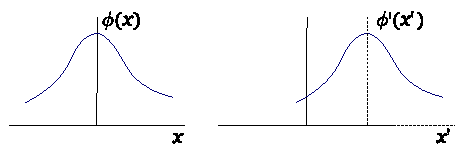
\includegraphics{trasla} %noinstiki
%   \caption{Traslaci\'on de funci\'on y coordenadas en una dimensi\'on: $\phi(x)=\phi'(x')$ } %noinstiki
%   \label{fig:trasla} %noinstiki
% \end{figure} %noinstiki<div id="fig:trasla">Figura trasla:Traslaci\'on de funci\'on y coordenadas $\phi(x)=\phi(x')$ </div>
% %noinstiki![trasla](http://gfif.udea.edu.co/figfs/trasla.png)
% %noinstiki
% Si $a^\mu$ es constante (un an\'alisis m\'as general es hecho en \cite{r})
% \begin{equation}
%   d^4x'=d^4x
% \end{equation}
% En este caso, asumiendo que el campo satisface las ecuaciones de
% Euler-Lagrange y usando la ec.~\eqref{eq:dmuxmu} y (\ref{eq:eelcallfmu}) tenemos
% \begin{align}
%   \delta S&=\int_{R}d^4x\,\mathcal{L}(\phi',\partial_\mu\phi',x')-\int_{R}d^4x\,\mathcal{L}(\phi(x),\partial_\mu\phi(x),x)\nonumber\\
%   &=\int_{R}d^4x\,\mathcal{L}(\phi+\delta\phi,\partial_\mu\phi+\partial_\mu(\delta\phi),x+\delta a)-\int_{R}d^4x\,\mathcal{L}\nonumber\\
%   &\approx\int_{R}d^4x\,
%   \left[\mathcal{L}+
%     \frac{\partial\mathcal{L}}{\partial\phi}\delta\phi+\frac{\partial\mathcal{L}}{\partial(\partial_\mu\phi)}\partial_\mu(\delta\phi)+
%     (\partial_\mu\mathcal{L})\delta a^\mu\right]-\int_{R}d^4x\,\mathcal{L}\nonumber\\
%   &=\int_{R}d^4x\,
%   \left[
%     \frac{\partial\mathcal{L}}{\partial\phi}\delta\phi+\frac{\partial\mathcal{L}}{\partial(\partial_\mu\phi)}\partial_\mu(\delta\phi)+
%     (\partial_\mu\mathcal{L})\delta a^\mu\right]\nonumber\\
%   &=\int_{R}d^4x\,
%   \left\{ 
%     \left[\partial_\mu\left(\frac{\partial\mathcal{L}}{\partial(\partial_\mu\phi)}
%     \right)\right]\delta\phi+\frac{\partial\mathcal{L}}{\partial(\partial_\mu\phi)}\partial_\mu(\delta\phi)+
%     (\partial_\mu\mathcal{L})\delta a^\mu\right\}\nonumber\\
%   &=\int_{R}d^4x\left\{ 
%     \partial_\mu\left[\frac{\partial\mathcal{L}}{\partial(\partial_\mu\phi)}\delta\phi\right]
%   +(\partial_\mu\mathcal{L})\delta a^\mu\right\}\nonumber\\
%   &=\int_{R}d^4x\,
%     \partial_\mu\left[
%       -\frac{\partial\mathcal{L}}{\partial(\partial_\mu\phi)}(\partial_\nu\phi)
%       +\delta^\mu_\nu\mathcal{L}
%     \right]\delta a^\nu\nonumber\\
%     \label{eq:2}
%   &=\int_{R}d^4x\,
%   \left(
%     \partial_\mu T^\mu_\nu
%   \right)\delta a^\nu=0.
% \end{align}
% Y por consiguiente
% \begin{equation}
%   \label{eq:131}
%   \partial_\mu T^\mu_\nu=0,
% \end{equation}
% donde
% \begin{equation}
%   \label{eq:tmunu}
%     T^\mu_\nu=\frac{\partial\mathcal{L}}{\partial(\partial_\mu\phi)}(\partial_\nu\phi)
%       -\delta^\mu_\nu\mathcal{L}
% \end{equation}
% El tensor $T^\mu_\nu$ proviene de asumir la homogeneidad del espacio y el tiempo y es llamado el tensor de momentum--energ\'\i a. 
% La densidad Hamiltonina se obtiene de $T^0_0$
% \begin{align}
%   \label{eq:3}
% \mathcal{H}&=T^0_0=\frac{\partial\mathcal{L}}{\partial\dot{\phi}}\dot{\phi}
%       -\mathcal{L}\\
%       &=\pi(x)\frac{\partial\phi(x)}{\partial t}-\mathcal{L}.
% \end{align}
% Comparando con la expresi\'on correspondiente en la formulaci\'on
% Lagrangiana de la Mec\'anica Cl\'asica, tenemos que si $\phi(x)$ es la
% variable can\'onica, la variable can\'onica conjugada es $\pi(x)$
% \begin{equation}
%   \label{eq:4}
%   \pi(x)=\frac{\partial\mathcal{L}}{\partial(\partial\phi(x)/\partial t)}.
% \end{equation}
% El teorema de Noether en este caso establece que la invarianza de la Acci\'on bajo traslaciones temporales da lugar a la ecuaci\'on de continuidad (\ref{eq:131}) para $\nu=0$
% \begin{align}
% \label{eq:122}
%   \partial_\mu T^\mu_0=0
% \end{align}
% cuya carga conservada corresponde a la energ\'\i a
% \begin{align}
%   H=\int_V d^3x\, T^0_0=\int_V d^3x\,\mathcal{H}.
% \end{align}
% De igual forma la invarianza bajo traslaciones espaciales de lugar a ecuaciones de continuidad para cada componente $\nu=i$
%  ($i=1,2,3$)
%  \begin{align}
%    \label{eq:235}
%    \partial_\mu T^\mu_i=0,
%  \end{align}
% cuyas densidad de cargas conservadas, $T^0_i$, que en forma vectorial escribiremos como $\mathbf{T}^0$, dan lugar a la conservaci\'on del momentum
% \begin{align}
%   \mathbf{P}=\int_V d^3x\,\mathbf{T}^0\,.
% \end{align}
% Generalizando a un campo complejo
% \begin{equation}
%   \label{eq:138}
%      T^\mu_\nu=\frac{\partial\mathcal{L}}{\partial(\partial_\mu\phi)}(\partial_\nu\phi)+(\partial_\nu\phi^*)\frac{\partial\mathcal{L}}{\partial(\partial_\mu\phi^*)}
%       -\delta^\mu_\nu\mathcal{L}
% \end{equation}
% \end{frame}

Note que las ecuaciones de Euler-Lagrange surgen del Problema variacional de Noether cuando se impone la parte inversa del primer teorema de Noether, es decir, aparecen cuando se imponen que las cargas se conserven como consecuencia de la condición
\begin{align}
   \sum_i \partial_{\mu} j^{\mu}_{\alpha i}=0\,.
\end{align}



\section{Campo escalar complejo}
%% Mover al otro capítulo

\begin{frame}[fragile,allowframebreaks]
En el caso de un campo de materia complejo, invariante bajo una simetría local $U(1)$ con parámetro $\theta(x)$, tenemos que $\phi_1\to \phi$, $\phi_2\to \phi^{*}$, de modo que $a_2=a_1^{*}$ y $b_1=b_2=0$. Entonces, el Teorema 2  de Noether aplicado a los campos $\phi$ y $\phi^{*}$ queda
\begin{align}
  \label{eq:th2mf}
   \sum_i \mathcal{E}_ia_i=&\sum_i  \partial_{\mu}   \left(  \mathcal{E}_i b^{\mu}_i  \right) = 0\,.
\end{align}
De modo que
\begin{align}
 \sum_i \mathcal{E}_ia_i=&\sum_i \left\{ \partial_{\mu} \left[ \frac{\partial\mathcal{L}}{\partial(\partial_{\mu}\phi_i)}\right]-\frac{\partial\mathcal{L}}{\partial\phi_i} \right\}a_i \nonumber\\
=&\sum_i \left\{ \partial_{\mu} \left[ \frac{\partial\mathcal{L}}{\partial(\partial_{\mu}\phi_i)}\right]a_i-\frac{\partial\mathcal{L}}{\partial\phi_i}a_i \right\} \nonumber\\
=&\sum_i \left\{ \partial_{\mu} \left[ \frac{\partial\mathcal{L}}{\partial(\partial_{\mu}\phi_i)}a_i\right]-\frac{\partial\mathcal{L}}{\partial(\partial_{\mu}\phi_i)}\partial_{\mu}a_i-\frac{\partial\mathcal{L}}{\partial\phi_i}a_i \right\}\,.
\end{align}
\end{frame}

\begin{frame}[fragile,allowframebreaks]
Teniendo en cuenta que como veremos más adelante en el capítulo~\ref{}, sec.~\ref{sec:invarianza-de-fase}, para un campo complejo
\begin{align}
  \label{eq:identityth2}
\sum_i \left[\frac{\partial\mathcal{L}}{\partial(\partial_{\mu}\phi_i)}\partial_{\mu}a_i+\frac{\partial\mathcal{L}}{\partial\phi_i}a_i \right]=0
\end{align}
Entonces, 
\begin{align}
\sum_i \mathcal{E}_ia_i=\partial_{\mu} j^{\mu}\,,
\end{align}
donde
\begin{align}
\label{eq:tnoeth2}
j^\mu=\sum_i\frac{\partial\mathcal{L}}{\partial(\partial_{\mu}\phi_i)}a_{i}\,.
\end{align}
Además, debido a la ec.~\eqref{eq:th2mf},
\begin{align}
  \partial_{\mu} j^{\mu}=0\,.
\end{align}


Este resultado particular para campos complejos se mantiene en general para el conjunto de campos que dependan sólo del parámetro y no de la derivada del parámetro, es decir, el conjunto de campos de materia con $b_i^\mu=0$: ver Teorema 3 de \cite{Brading:2000hc}. Note que la corriente conservada para el campo de materia asociada a una transformación local coincide con la corriente conservada para una transformación global dada en la ec.~\eqref{eq:th1ng}.


Sin embargo, la conservación de la carga en este caso no requiere imponer que $\mathcal{E}_i=0$. Por lo tanto el caso de la conservación de carga \emph{impropia} se puede considerar más fundamental e inviolable. Esto nos permite formular el \emph{principio gauge} como la necesidad de establecer Lagrangianos que respetan las simetría internas a nivel local.
\end{frame}


Cuando la conservación de la carga requiera de que las ecuaciones de Euler-Lagrange se satisifagan, diremos que la conservación de la carga es \emph{propia}.

\section{Ecuación de Klein-Gordon}


Si modificamos el Lagrangiano en ec.~\eqref{eq:call2}, para incluir un
t\'ermino adicional ($v=c=1$)
\begin{equation}
  \label{eq:14}
  \mathcal{L}(\partial\phi/\partial t,\partial\phi/\partial z)=\frac{1}{2}
\left[
  \left(\frac{\partial\phi}{\partial t}\right)^2-\left(\frac{\partial\phi}{\partial z}\right)^2-m^2\phi^2
\right].
\end{equation}
entonces, la ec.~\eqref{eq:12} es soluci\'on a la ecuaci\'on resultante de
aplicar las ecuaciones de Euler-Lagrange:
\begin{align}
\label{eq:150}
      \frac{\partial^2\phi}{\partial t^2}-\frac{\partial^2\phi}{\partial z^2}+m^2\phi=&0\nonumber\\
      \left(\frac{\partial^2}{\partial t^2}-\frac{\partial^2}{\partial z^2}+m^2
      \right)\phi=&0,
\end{align}

Generalizando a 3 dimensiones tenemos el Lagrangiano de Klein-Gordon
\begin{align}
  \label{eq:15}
  \mathcal{L}=&\frac12 \partial_{\mu}\phi\partial^{\mu}\phi-\frac12 m^2\phi^{2}\nonumber\\
=&\frac{1}{2}
  \left(
\frac{\partial\phi}{\partial t}
  \right)^2-\tfrac{1}{2}\boldsymbol{\nabla}\phi\cdot\boldsymbol{\nabla}\phi-\tfrac{1}{2}m^2\phi^2,
\end{align}
que dan lugar a la ecuaci\'on de Klein-Gordon

\begin{equation}
\label{eq:152}
  \left(
\frac{\partial^2}{\partial t^2}-\nabla^2+m^2
  \right)\phi=0.
\end{equation}

Una forma de derivar la ecuación de Schr\"odinger es usar escribir la ecuación de conservación de la energía mecánica en términos de operadores aplicados a la función de onda
\begin{align}
  \widehat{H}\psi=\left( \frac{1}{2m}\widehat{\mathbf{p}}^{2}+v \right)\psi\,,
\end{align}

De esta manera, la versión mecánico cuántica de la conservación de momentum-energía de la relatividad especial se podría obtener de
\begin{align}
  \widehat{p}_{\mu}\widehat{p}\;^{\mu}\psi=&\left( \widehat{H}^{2}-\sum_{i}\widehat{p}\;^i\widehat{p}\;^i \right)\psi \nonumber\\
=&\left( -\partial_0^2+\nabla^2 \right)\psi \nonumber\\
=& m^2 \psi\,,
\end{align}
de donde obtenemos precisamente la ecuación~\eqref{eq:152}
\begin{align}
  \left(
\frac{\partial^2}{\partial t^2}-\nabla^2+m^2
  \right)\psi=0.
\end{align}
Aunque la interpretación en mecánica cuántica de la ecuación de momentum-energía requiere promover también el campo a un operador, una vez se establece la teoría cuántica de campos correspondiente, el coeficiente $m$ se puede interpretar como la masa del campo $\psi$.




% \begin{subappendices}
  
% \end{subappendices}
 



\section{Problemas}
\label{sec:problemas-2}
\renewcommand{\labelenumi}{\thechapter.\theenumi} %noinstiki
\begin{enumerate}
\item  Mostrar la invarianza del producto escalar para la definición del producto escalar $\operatorname{SU}(2)$
\begin{align}
   \Psi\cdot \Psi \equiv \Psi^{\dagger}\Psi\,.
\end{align}

\item Demostrar que $\Lambda(\xi_1)$ dada en la primera ec.~\eqref{eq:Lximunu},  cumple la condición de ortogonalidad generalizada~\eqref{eq:cdeog}.

\item Muestre que bajo los cambios $\xi\to i\theta$ y $t\to it$, la transformación de Lorentz se puede escribir como una matriz de rotación convencional.

\item  Demuestre que la ecuación de Klein-Gordon en \eqref{eq:KG} proviende de una densidad Lagragiana del tipo
\begin{align}
  \mathcal{L}(\phi,\partial_{\mu} \phi)=  \frac{1}{2}{\partial_\mu\phi}\,{\partial^\mu\phi}-V(\phi)\,,
\end{align}
donde
\begin{align}
  V(\phi)=\frac{1}{2}m^2 \phi^2\,.
\end{align}

  
  
\item Muestre que
  \begin{equation*}
    {\Lambda^{\mu}}_{\nu}{\Lambda_\mu}^{\rho}={\Lambda_{\mu}}^{\nu}{\Lambda^{\mu}}_{\rho}=\delta^\rho_\nu
  \end{equation*}
Compruebe esta identidad para la transformaci\'on de Lorentz de la ec.~\eqref{eq:147}
\label{item:pch2.1} %noinstiki

  
\item Obtenga el Hamiltoniano a partir de Lagrangiano en\eqref{eq:238} y encuentre la expresi\'on para la densidad Lagrangiana en t\'erminos de $\phi$.
\label{item:pch1.0} %noinstiki
% \item Demuestre las ecuaciones (\ref{eq:237})(\ref{eq:236}).
% \label{item:pch1.1} %noinstiki



% \item A partir del Lagrangiano de la Mec\'anica Cu\'antica invariante bajo transformaciones de fase local encuentre la ecuaci\'on de Schr\"odinger en presencia del campo electromagn\'etico. Ver secci\'on \ref{sec:aplic-la-mecan}.

\item Para la densidad Lagrangiana de Scrödinger
    \begin{align}
      \mathcal{L}(\psi,\psi^*,\partial_\mu\psi,\partial_\mu\psi^*)
&=\frac{1}{2m}\boldsymbol{\nabla}\psi^*\cdot\boldsymbol{\nabla}\psi-\frac{i}{2}
  \left(
\psi^*\frac{\partial\psi}{\partial t}-\frac{\partial\psi^*}{\partial t}\psi
  \right)+\psi^*V\psi\,.
  \end{align}

\begin{enumerate}
\item Calcule las ecuaciones de Euler-Lagrange 
\item Calcule la carga de corriente conservada asociada al cambio de fase 

\item Calcule el tensor de momento energía

\end{enumerate}
  
\item Calcule $T^i_0$ para el Lagrangiano de Schr\"odinger
  \begin{align}
    T^i_0=&\frac{\partial\mathcal{L}}{\partial(\partial_i \psi)}\partial_0\psi+\partial_0\psi^*\frac{\partial\mathcal{L}}{\partial(\partial_i \psi^*)}\nonumber\\
    =&\frac{1}{2m}\left(\partial_i\psi^*\partial_0\psi+\partial_0\psi^*\partial_i\psi \right)
  \end{align}
De modo que $T^0_i\neq T^i_0$.

\end{enumerate}


\renewcommand{\labelenumi}{\theenumi} %noinstiki
% \left(\right)
%%% Local Variables: 
%%% mode: latex
%%% TeX-master: "fullnotes"
%%% ispell-local-dictionary: "castellano8"
%%% End: